\documentclass[11pt,letterpaper]{article}
\usepackage[english]{babel}
 
\usepackage{letltxmacro}
\usepackage{latexsym}
\usepackage{booktabs}
\usepackage{siunitx}
\usepackage{multirow}
\usepackage{algpseudocode}
\usepackage{array}
\usepackage{tabularx}

\sisetup{
  separate-uncertainty = true,
  table-number-alignment = center
}
\LetLtxMacro{\ORIGselectlanguage}{\selectlanguage}
\makeatletter
\DeclareRobustCommand{\selectlanguage}[1]{%
  \@ifundefined{alias@\string#1}
    {\ORIGselectlanguage{#1}}
    {\begingroup\edef\x{\endgroup
       \noexpand\ORIGselectlanguage{\@nameuse{alias@#1}}}\x}%
}
\newcommand{\definelanguagealias}[2]{%
  \@namedef{alias@#1}{#2}%
}
\makeatother
 
 
\definelanguagealias{en}{english}
\definelanguagealias{English}{english}
\usepackage{graphicx}
\usepackage{amsmath}
\usepackage{amsfonts}
\usepackage{amssymb}
\usepackage{amsthm}
\usepackage{cancel}
\usepackage{mathtools}
\usepackage{bm}

\usepackage[percent]{overpic}
\usepackage[dvipsnames]{xcolor}
\usepackage{soul}
\usepackage{wasysym}
\usepackage{dsfont}
\usepackage{physics}
\AtBeginDocument{\RenewCommandCopy\qty\SI} 
% natbib must precede hyperref. It drives this document's own reference
% list, which apsrev4-2.bst formats in the same style as the main article.
\usepackage[numbers,sort&compress]{natbib}
\usepackage{hyperref}
\hypersetup{colorlinks,allcolors=black}
\usepackage{comment}
\usepackage{enumitem}
\usepackage{textgreek}
\usepackage{tcolorbox}
 
\newcounter{alg}
 
\hypersetup{
  colorlinks   = true,
  urlcolor     = blue,
  linkcolor    = blue,
  citecolor    = red
}
\usepackage[mathscr]{euscript}
 
\usepackage{varwidth}
\usepackage[lined,boxed,ruled,norelsize,linesnumbered]{algorithm2e}
\usepackage{verbatim}
\usepackage[normalem]{ulem}
\usepackage{cleveref}
 
\renewcommand{\algorithmicrequire}{\textbf{Input:}}
\renewcommand{\algorithmicensure}{\textbf{Output:}}
 
% ============================================================
%  Theorem-like environments
% ============================================================
\newtheorem{theorem}{Theorem}
\newtheorem{result}{Result}
\newtheorem{lemma}{Lemma}
\newtheorem{problem}{Problem}
\newtheorem{proposition}{Proposition}
\newtheorem{remark}{Remark}
\newtheorem{assumption}{Assumption}
\newtheorem{definition}{Definition}
\newtheorem{fact}{Fact}
\newtheorem*{lemma*}{Lemma}
\newtheorem{corollary}{Corollary}
\newtheorem*{theorem*}{Theorem}
\newtheorem{thm}{\protect\theoremname}
\theoremstyle{plain}
\newtheorem{lem}{\protect\lemmaname}
\theoremstyle{plain}
\newtheorem{rem}[thm]{\protect\remarkname}
\theoremstyle{plain}
\newtheorem*{lem*}{\protect\lemmaname}
\theoremstyle{plain}
\newtheorem*{thm*}{\protect\theoremname}
\theoremstyle{plain}
\newtheorem{prop}[thm]{\protect\propositionname}
\theoremstyle{plain}
\newtheorem{cor}[thm]{\protect\corollaryname}
\newtheorem{defn}{Definition}
\newtheorem{prob}[thm]{Problem}
\newtheorem{notation}[thm]{Notation}
 
\newtheorem{manualtheoreminner}{Theorem}
\newenvironment{manualtheorem}[1]{%
  \renewcommand\themanualtheoreminner{#1}%
  \manualtheoreminner
}{\endmanualtheoreminner}
 
\renewcommand{\thealg}{\arabic{alg}}
\newtcolorbox[use counter=alg,
              crefname={algorithm}{algorithms},
              Crefname={Algorithm}{Algorithms}]
{alg}[2][]{%
  floatplacement=#1,
  float,
  colback=cyan!5!white,
  colframe=cyan!50!black,
  colbacktitle=cyan!85!black,
  fonttitle=\bfseries,
  title=Algorithm~\thealg: #2
}
 
\renewcommand{\topfraction}{0.95}
\renewcommand{\bottomfraction}{0.95}
\renewcommand{\textfraction}{0.05}
\renewcommand{\floatpagefraction}{0.9}
\setcounter{topnumber}{10}
\setcounter{bottomnumber}{10}
\setcounter{totalnumber}{20}
 

\NewDocumentCommand{\hyh}{m}{\textcolor{purple}{[HYH: #1]}}
\definecolor{mycrimson}{HTML}{A60808}
\NewDocumentCommand{\elo}{m}{\textcolor{mycrimson}{[ELO: #1]}}
\NewDocumentCommand{\sfy}{m}{\textcolor{teal}{[SFY: #1]}}
\newcommand{\EPR}{\mathrm{EPR}}
\newcommand{\eq}[1]{\begin{equation}#1\end{equation}}
\newcommand{\eqs}[1]{\begin{equation}\begin{split}#1\end{split}\end{equation}}
\newcommand{\eqnref}[1]{Eq.\,\eqref{#1}}
\newcommand{\figref}[1]{Fig.\,\ref{#1}}
\newcommand{\tabref}[1]{Tab.\,\ref{#1}}
\newcommand{\secref}[1]{Sec.\,\ref{#1}}
\newcommand{\appref}[1]{Appendix\,\ref{#1}}
\newcommand{\refcite}[1]{Ref.\,\cite{#1}}
\newcommand{\ii}{\mathrm{i}}
\newcommand{\ee}{\mathrm{e}}
\newcommand{\cd}[1]{c^{\dagger}_{#1}}
\newcommand{\cc}[1]{c_{#1}}
\newcommand{\moy}[1]{\langle #1 \rangle}
\newcommand{\sandwich}[3]{\mbox{$ \langle #1 | #2 | #3 \rangle $}}
\newcommand{\red}[1]{{\color{red} #1}}
\DeclareMathOperator*{\bigrarrow}{\rightarrow}
\DeclareMathOperator*{\biglongrarrow}{\longrightarrow}
 
\setlength{\belowcaptionskip}{-10pt}
\setlength{\skip\footins}{24pt}
\raggedbottom
 
\usepackage{bbm}
\usepackage{tikz-cd}

\newcommand{\C}{\mathbb{C}}
\newcommand{\R}{\mathbb{R}}
\newcommand{\N}{\mathbb{N}}
\newcommand{\Z}{\mathbb{Z}}
\newcommand{\End}{\mathrm{End}}
\newcommand{\Hom}{\mathrm{Hom}}
\newcommand{\Lie}{\mathrm{Lie}}
\newcommand{\ad}{\mathrm{ad}}
\newcommand{\id}{\mathrm{id}}
\newcommand{\gl}{\mathfrak{gl}}
\newcommand{\su}{\mathfrak{su}}
\newcommand{\uu}{\mathfrak{u}}
\newcommand{\slc}{\mathfrak{sl}}
\newcommand{\HH}{\mathcal{H}}
\newcommand{\I}{\mathbbm{1}}
\newcommand{\boxt}{\boxtimes}
\newcommand{\Proj}{\Pi}

\theoremstyle{plain}
\newtheorem{smtheorem}{Theorem}[section]
\newtheorem{smproposition}[smtheorem]{Proposition}
\newtheorem{smlemma}[smtheorem]{Lemma}
\newtheorem{smcorollary}[smtheorem]{Corollary}
\theoremstyle{definition}
\newtheorem{smdefinition}[smtheorem]{Definition}
\newtheorem{smremark}[smtheorem]{Remark}
\newtheorem{smexample}[smtheorem]{Example}
\theoremstyle{plain}


% ---- Supplemental Material specific ------------------------------------
\usepackage[letterpaper,margin=1in]{geometry}
\geometry{margin=0.5in}

% Resolve \ref{...} that point into the main article. Citations are NOT
% shared: this document carries its own reference list, because APS posts
% Supplemental Material as a separate, self-contained file.
\usepackage{xr}
% Neutralize \bibcite while xr reads main.aux, so the main article's
% reference numbers do not clash with this document's own.
\makeatletter
\let\SM@bibcite\bibcite
\let\bibcite\@gobbletwo
\externaldocument{main}
\let\bibcite\SM@bibcite
\makeatother
% xr and hyperref together leave \XR@prefix undefined at \cite time;
% it is empty whenever \externaldocument is used without a label prefix.
\makeatletter
\providecommand\XR@prefix{}
\makeatother

% "S" prefix so that every number quoted in the main text is unambiguously
% a Supplemental Material number.
\renewcommand{\thesection}{S\arabic{section}}
\renewcommand{\theequation}{S\arabic{equation}}
\renewcommand{\thefigure}{S\arabic{figure}}
\renewcommand{\thetable}{S\arabic{table}}
\renewcommand{\bibnumfmt}[1]{[S#1]}
\renewcommand{\citenumfont}[1]{S#1}
% ------------------------------------------------------------------------


\begin{document}

\title{Supplemental Material for\\[0.3em]
\textit{Covariant Approximate Quantum Codes for Protected Analog Computation}}

\author{Mariia Elovenkova, Hong-Ye Hu, and Susanne F. Yelin\\[0.3em]
\normalsize Department of Physics, Harvard University, Cambridge, MA 02138, USA}

\date{}

\maketitle

\tableofcontents
\clearpage

\section*{Nomenclature}\label{sec:notation}
\subsection*{Hilbert spaces, channels, and encoding maps}

\begin{tabular}{@{}ll@{}}

\parbox[t]{0.22\textwidth}{$\mathcal{H}$} & \parbox[t]{0.72\textwidth}{A finite-dimensional Hilbert space.} \\[0.6em]

\parbox[t]{0.22\textwidth}{$\mathcal{H}_L$} & \parbox[t]{0.72\textwidth}{A finite-dimensional logical Hilbert space.} \\[0.6em]

\parbox[t]{0.22\textwidth}{$\mathcal{H}_P$} & \parbox[t]{0.72\textwidth}{A finite-dimensional physical Hilbert space.} \\[0.6em]

\parbox[t]{0.22\textwidth}{$\mathcal{N}, \mathcal{M}$} & \parbox[t]{0.72\textwidth}{Quantum channels, i.e. completely positive trace-preserving linear maps.} \\[0.6em]

\parbox[t]{0.22\textwidth}{$\mathcal{E}$} & \parbox[t]{0.72\textwidth}{An encoding map from a logical Hilbert space to a physical Hilbert space.} \\[0.6em]

\parbox[t]{0.22\textwidth}{$\mathcal{V}$} & \parbox[t]{0.72\textwidth}{An encoding isometry, corresponding to encoding map $\mathcal{E}$, i. e. $\mathcal{E}(\rho_L)=\mathcal{V}\rho_L\mathcal{V}^{\dagger}$.} \\[0.6em]

\parbox[t]{0.22\textwidth}{$\rho^{(i)}(\rho_L)$} & \parbox[t]{0.72\textwidth}{The reduced state on the $i$-th physical qudit after encoding, i. e. $\rho^{(i)}(\rho_L)=\mathrm{Tr}_{\hat{i}}(\mathcal{V}\rho_L\mathcal{V}^{\dagger})$.} \\[0.6em]

\parbox[t]{0.22\textwidth}{$A_i$, $A_S$} & \parbox[t]{0.72\textwidth}{The Hilbert space of the $i$-th physical qudit, and $A_S=\bigotimes_{i\in S}A_i$ for a subset $S\subseteq\{1,\ldots,n\}$.} \\[0.6em]

\parbox[t]{0.22\textwidth}{$\hat S$} & \parbox[t]{0.72\textwidth}{The complement of $S$ in $\{1,\ldots,n\}$. The hat marks complementation generally: $\widehat{ijk}$ for the complement of $\{i,j,k\}$, $\widehat j$ for the retained tensor factors other than $j$, and $\widehat{\mathcal N}$ for the complementary channel.} \\[0.6em]

\parbox[t]{0.22\textwidth}{$\rho^{(S)}(\rho_L)$} & \parbox[t]{0.72\textwidth}{The reduced state on $A_S$ after encoding, i.\,e. $\rho^{(S)}(\rho_L)=\operatorname{Tr}_{\hat S}(\mathcal{V}\rho_L\mathcal{V}^\dagger)$, see Eq.~\eqref{eq:reduced_state}.} \\[0.6em]

\parbox[t]{0.22\textwidth}{$\widehat{\mathcal{N}}$} & \parbox[t]{0.72\textwidth}{The complementary channel to $\mathcal{N}$, see definition \ref{def:complementary_channel}.} \\[0.6em]

\parbox[t]{0.22\textwidth}{$f(\rho, \sigma)$} & \parbox[t]{0.72\textwidth}{The fidelity between states $\rho$ and $\sigma$, see definition \ref{def:root_fidelity}.} \\[0.6em]

\parbox[t]{0.22\textwidth}{$F_{\rho}(\mathcal{N}, \mathcal{M})$} & \parbox[t]{0.72\textwidth}{The entanglement fidelity between channels $\mathcal{N}$ and $\mathcal{M}$, see definition \ref{def:rho_entanglement_fidelity}.} \\[0.6em]

\parbox[t]{0.22\textwidth}{$F(\mathcal{N}, \mathcal{M})$} & \parbox[t]{0.72\textwidth}{The worst-case entanglement fidelity between channels $\mathcal{N}$ and $\mathcal{M}$, see definition \ref{def:worst_case_entanglement_fidelity}.} \\[0.6em]

\parbox[t]{0.22\textwidth}{$\ket{\psi_\rho}$} & \parbox[t]{0.72\textwidth}{A purification of the state $\rho$ on the logical space, used as the reference-assisted input in $F_\rho$.} \\[0.6em]

\parbox[t]{0.22\textwidth}{$d(\mathcal N,\mathcal M)$} & \parbox[t]{0.72\textwidth}{The fidelity-induced channel distance $\sqrt{1-F(\mathcal N,\mathcal M)}$, see Eq.~\eqref{eq:distance_def}.} \\[0.6em]

\parbox[t]{0.22\textwidth}{$\|\cdot\|_\diamond$} & \parbox[t]{0.72\textwidth}{The diamond norm, i.\,e. the completely bounded trace norm on linear maps between operator spaces.} \\[0.6em]

\parbox[t]{0.22\textwidth}{$\Lambda_0$} & \parbox[t]{0.72\textwidth}{A constant channel, i.\,e. $\Lambda_0(\rho)=\operatorname{Tr}(\rho)\rho_0$ for a fixed state $\rho_0$, see Eq.~\eqref{eq:constant_channel_def}.} \\[0.6em]

\parbox[t]{0.22\textwidth}{$\mathcal R_p$} & \parbox[t]{0.72\textwidth}{A recovery channel for flagged $k$-site erasure with distribution $p=(p_S)_{|S|=k}$ over the erased sets, Eq.~\eqref{eq:erasure_noise}.} \\[0.6em]

\parbox[t]{0.22\textwidth}{$\widehat{\mathcal N}_S$} & \parbox[t]{0.72\textwidth}{A complementary channel to the local noise channel $\mathcal N_S$ acting on $A_S$.} \\[0.6em]

\parbox[t]{0.22\textwidth}{$\tau_S$, $\Delta_S$} & \parbox[t]{0.72\textwidth}{The logical-independent and logical-dependent parts of the reduced state on $A_S$, i.\,e. $\rho^{(S)}(\rho_L)=\tau_S+\Delta_S(\rho_L)$, see Eq.~\eqref{eq:leakage-splitting}.} \\[0.6em]

\parbox[t]{0.22\textwidth}{$\delta$} & \parbox[t]{0.72\textwidth}{The uniform leakage of a code over a family of subsets, see Eq.~\eqref{eq:uniform-leakage}.} \\[0.6em]

\parbox[t]{0.22\textwidth}{$\mathcal{V}_0$} & \parbox[t]{0.72\textwidth}{The seed isometry placing the logical qudit at site $0$ and filling the rest with $SU(d)$-singlets, see Eq.~\eqref{eq:seed-isometry}.} \\[0.6em]

\parbox[t]{0.22\textwidth}{$\mathcal{V}_m$, $\mathcal E_m$} & \parbox[t]{0.72\textwidth}{The encoding isometry built from the multiplicity vector $\ket m$ and the corresponding encoding $\mathcal E_m(X)=\mathcal{V}_mX\mathcal{V}_m^\dagger$, see Eq.~\eqref{eq:Vm}.} \\[0.6em]

\parbox[t]{0.22\textwidth}{$\mathcal E_s$} & \parbox[t]{0.72\textwidth}{The encoding $\mathcal E_s(X)=\mathcal{V}_{m_s}X\mathcal{V}_{m_s}^\dagger$ built from the efficiently sampled multiplicity vector $\ket{m_s}$.} \\[0.6em]

\parbox[t]{0.22\textwidth}{$\Phi_{S,m}$} & \parbox[t]{0.72\textwidth}{The erased-subsystem channel $\Phi_{S,m}(X)=\operatorname{Tr}_{\hat S}(\mathcal{V}_mX\mathcal{V}_m^\dagger)$, i.\,e. the reduced-state map $\rho^{(S)}$ for the code $\mathcal E_m$, see Eq.~\eqref{eq:local-channel}.} \\[0.6em]

\parbox[t]{0.22\textwidth}{$\overline\Phi_{k,n}$} & \parbox[t]{0.72\textwidth}{The mean $k$-site channel, i.\,e. the Haar average of $\Phi_{S,m}$ over the multiplicity vector $\ket m$.} \\[0.6em]

\parbox[t]{0.22\textwidth}{$\lambda_{k,n}$, $\Lambda_{k,n}$} & \parbox[t]{0.72\textwidth}{The state $\overline\Phi_{k,n}(\tau)$ and the constant channel $\Lambda_{k,n}(X)=\operatorname{Tr}(X)\lambda_{k,n}$ it defines, see Eq.~\eqref{eq:lambda-kn}.} \\[0.6em]

\end{tabular}


\subsection*{Spin systems and \(SU(2)\) notation}

\begin{tabular}{@{}ll@{}}

\parbox[t]{0.22\textwidth}{$V_j$} & \parbox[t]{0.72\textwidth}{The spin-$j$ irreducible representation of $SU(2)$.} \\[0.6em]

\parbox[t]{0.22\textwidth}{$J_x, J_y, J_z$} & \parbox[t]{0.72\textwidth}{The spin-$j$ generators of $SU(2)$ acting on $V_j$, see Eq.~\eqref{eq:spinj}, Eq.~\eqref{eq:Jz}, and Eq.~\eqref{eq:Jpm}.} \\[0.6em]

\end{tabular}


\subsection*{\(SU(d)\) generators and covariance notation}

\begin{tabular}{@{}ll@{}}

\parbox[t]{0.22\textwidth}{$t_a$} & \parbox[t]{0.72\textwidth}{The generators of $\mathfrak{su}(d)$, traceless Hermitian complex $d\times d$ matrices, see Eq.~\eqref{eq:sudgenerators}.} \\[0.6em]

\parbox[t]{0.22\textwidth}{$\bar{t}_a$} & \parbox[t]{0.72\textwidth}{The generators of $\mathfrak{su}(d)$ in the fundamental representation, used to emphasize action on the logical Hilbert space.} \\[0.6em]

\parbox[t]{0.22\textwidth}{$t_a^{(i)}$} & \parbox[t]{0.72\textwidth}{The generators of $\mathfrak{su}(d)$ in the fundamental representation acting on the $i$-th physical qudit.} \\[0.6em]

\parbox[t]{0.22\textwidth}{$T_a^{(i)}$} & \parbox[t]{0.72\textwidth}{The generators of $\mathfrak{su}(d)$ in the arbitrary representation acting on the $i$-th physical qudit.} \\[0.6em]

\parbox[t]{0.22\textwidth}{$T_a$} & \parbox[t]{0.72\textwidth}{The global generators of $\mathfrak{su}(d)$, acting on the whole physical space, see Eq.~\eqref{eq:global_generators}.} \\[0.6em]

\parbox[t]{0.22\textwidth}{$U_{\lambda_0}^{(i)}(g)$} & \parbox[t]{0.72\textwidth}{Representation of an element $g\in SU(d)$ on physical site $i$ equipped with irreducible representation $V_{\lambda_0}$ of $SU(d)$.} \\[0.6em]

\parbox[t]{0.22\textwidth}{$\pi_{\lambda_0}^{(i)}(X)$} & \parbox[t]{0.72\textwidth}{Representation of an element $X\in \mathfrak{su}(d)$ on physical site $i$ equipped with irreducible representation $V_{\lambda_0}$ of $\mathfrak{su}(d)$.} \\[0.6em]

\parbox[t]{0.22\textwidth}{$U_L(g)$, $U_P(g)$} & \parbox[t]{0.72\textwidth}{The unitary representations of $g\in G$ on the logical and physical Hilbert spaces, so that covariance reads $\mathcal{V}U_L(g)=U_P(g)\mathcal{V}$, see Eq.~\eqref{eq:group_covar_cond}.} \\[0.6em]

\parbox[t]{0.22\textwidth}{$u(g)$} & \parbox[t]{0.72\textwidth}{Fundamental representation of $g\in SU(d)$ on the logical space.} \\[0.6em]

\parbox[t]{0.22\textwidth}{$\mathrm{Ad}$} & \parbox[t]{0.72\textwidth}{The adjoint representation of $SU(d)$.} \\[0.6em]

\parbox[t]{0.22\textwidth}{$\delta_{a b}$} & \parbox[t]{0.72\textwidth}{The Kronecker delta.} \\[0.6em]

\parbox[t]{0.22\textwidth}{$d_{abc}$} & \parbox[t]{0.72\textwidth}{The symmetric structure constants of $\mathfrak{su}(d)$, see Eq.~\eqref{eq:sudgenerators}, Eq.~\eqref{eq:sudnormalisation}, Eq.~\eqref{eq:sudidentities}.} \\[0.6em]

\parbox[t]{0.22\textwidth}{$f_{abc}$} & \parbox[t]{0.72\textwidth}{The antisymmetric structure constants of $\mathfrak{su}(d)$, see Eq.~\eqref{eq:sudgenerators}, Eq.~\eqref{eq:sudidentities}.} \\[0.6em]

\parbox[t]{0.22\textwidth}{$E_{rs}$} & \parbox[t]{0.72\textwidth}{The matrix units, see Eq.~\eqref{eq:matr_units}.} \\[0.6em]

\parbox[t]{0.22\textwidth}{$F_{rs}$} & \parbox[t]{0.72\textwidth}{The traceless matrix units, see Eq.~\eqref{eq:matr_units}.} \\[0.6em]

\end{tabular}


\subsection*{Exterior powers and fundamental \(SU(d)\) representations}

\begin{tabular}{@{}ll@{}}

\parbox[t]{0.22\textwidth}{$\bigwedge^r \mathbb{C}^d$} & \parbox[t]{0.72\textwidth}{The $r$-th exterior power of $\mathbb{C}^d$.} \\[0.6em]

\parbox[t]{0.22\textwidth}{$u \wedge v$} & \parbox[t]{0.72\textwidth}{The wedge product of vectors $u$ and $v$ in $\mathbb{C}^d$.} \\[0.6em]

\parbox[t]{0.22\textwidth}{$\omega_r$} & \parbox[t]{0.72\textwidth}{Fundamental weights of $SU(d)$, see Remark~\ref{rem:fundamental_weights}.} \\[0.6em]

\parbox[t]{0.22\textwidth}{$V_{\omega_r}$} & \parbox[t]{0.72\textwidth}{The irreducible representation of $SU(d)$ with highest weight $\omega_r$, which is isomorphic to $\bigwedge^r \mathbb{C}^d$, see definition \ref{def:rfundSUd} and Remark~\ref{rem:fundamental_weights}.} \\[0.6em]

\parbox[t]{0.22\textwidth}{$\kappa_{\omega_r}$} & \parbox[t]{0.72\textwidth}{Dynkin index of the representation $V_{\omega_r}$, or, equivalently, the normalization constant, see Eq.~\eqref{eq:sudnormalisation_2}.} \\[0.6em]

\parbox[t]{0.22\textwidth}{$\ket{\zeta_d}$} & \parbox[t]{0.72\textwidth}{The normalized totally antisymmetric state of $d$ qudits, the unique $SU(d)$-invariant vector in $(V_{\omega_1})^{\otimes d}$, see Eq.~\eqref{eq:singlet}.} \\[0.6em]

\parbox[t]{0.22\textwidth}{$\tau$} & \parbox[t]{0.72\textwidth}{The maximally mixed state $I_d/d$ on a single physical qudit.} \\[0.6em]

\parbox[t]{0.22\textwidth}{$\tau_s$} & \parbox[t]{0.72\textwidth}{The projector onto $\bigwedge^sV_{\omega_1}$, equal to the reduced state of any $s$ tensor factors of $\ket{\zeta_d}$, see Eq.~\eqref{eq:tau-s}; $\tau_1=\tau$.} \\[0.6em]

\parbox[t]{0.22\textwidth}{$\beta_{\ell,N}$} & \parbox[t]{0.72\textwidth}{The $\ell$-site reduced state of the background $\ket{\zeta_d}\bra{\zeta_d}^{\otimes q}$ on a uniformly random ordered tuple of $\ell$ distinct sites, averaged over the tuple; evaluated in Proposition~\ref{prop:beta-partition}, Eq.~\eqref{eq:beta-partition}.} \\[0.6em]

\end{tabular}


\subsection*{Groups and Lie algebras}

\begin{tabular}{@{}ll@{}}

\parbox[t]{0.22\textwidth}{$GL_d(\mathbb{C})$} & \parbox[t]{0.72\textwidth}{The group of invertible $d \times d$ complex matrices.} \\[0.6em]

\parbox[t]{0.22\textwidth}{$SU(d)$} & \parbox[t]{0.72\textwidth}{The group of $d \times d$ unitary matrices with determinant $1$.} \\[0.6em]

\parbox[t]{0.22\textwidth}{$\mathfrak{g}$} & \parbox[t]{0.72\textwidth}{A Lie algebra.} \\[0.6em]

\parbox[t]{0.22\textwidth}{$\mathfrak{g}_\C$} & \parbox[t]{0.72\textwidth}{The complexification of a Lie algebra $\mathfrak{g}$, see Definition~\ref{def:complexification}.} \\[0.6em]

\parbox[t]{0.22\textwidth}{$\mathfrak{gl}(d)$} & \parbox[t]{0.72\textwidth}{The Lie algebra of $d \times d$ complex matrices.} \\[0.6em]

\parbox[t]{0.22\textwidth}{$\mathfrak{sl}(d)$} & \parbox[t]{0.72\textwidth}{The Lie algebra of $d \times d$ complex matrices with zero trace.} \\[0.6em]

\parbox[t]{0.22\textwidth}{$\mathfrak{u}(d)$} & \parbox[t]{0.72\textwidth}{The Lie algebra of $d \times d$ skew-Hermitian matrices.} \\[0.6em]

\parbox[t]{0.22\textwidth}{$\mathfrak{su}(d)$} & \parbox[t]{0.72\textwidth}{The Lie algebra of $d \times d$ skew-Hermitian matrices with zero trace.} \\[0.6em]

\parbox[t]{0.22\textwidth}{$\mathfrak{su}(\mathcal{H})$} & \parbox[t]{0.72\textwidth}{The Lie algebra of skew-Hermitian traceless operators on \(\mathcal H\); if \(\dim\mathcal H=d\), then \(\mathfrak{su}(\mathcal H)\cong\mathfrak{su}(d)\).} \\[0.6em]

\parbox[t]{0.22\textwidth}{$\mathfrak{u}(1)$} & \parbox[t]{0.72\textwidth}{One-dimensional Lie algebra of purely imaginary numbers.} \\[0.6em]

\parbox[t]{0.22\textwidth}{$\Lie_{\R}\{i H_0, i H_1, \ldots, i H_k\}$} & \parbox[t]{0.72\textwidth}{The real Lie algebra generated by the set of Hamiltonians by nested commutators.} \\[0.6em]

\end{tabular}


\subsection*{Linear maps, intertwiners, and representation spaces}

\begin{tabular}{@{}ll@{}}

\parbox[t]{0.22\textwidth}{$V$, $W$} & \parbox[t]{0.72\textwidth}{Finite-dimensional complex vector spaces, or $G$-representations, when no particular one is meant; in the $SU(d)$ sections $V\cong\mathbb C^d$ carries the defining action, so that $S_\lambda(V)$ and $\Lambda^rV$ are its Schur functors and exterior powers.} \\[0.6em]

\parbox[t]{0.22\textwidth}{$\Hom_{\C}(V, W)$} & \parbox[t]{0.72\textwidth}{The space of complex linear maps from $V$ to $W$.} \\[0.6em]

\parbox[t]{0.22\textwidth}{$\End_{\C}(V)$} & \parbox[t]{0.72\textwidth}{The space of complex linear maps from $V$ to itself.} \\[0.6em]

\parbox[t]{0.22\textwidth}{$\End_{\C}(V)^G$} & \parbox[t]{0.72\textwidth}{The space of $G$-invariant complex linear maps from $V$ to itself.} \\[0.6em]

\parbox[t]{0.22\textwidth}{$\Hom_G(V, W)$} & \parbox[t]{0.72\textwidth}{The space of $G$-covariant linear maps from $V$ to $W$.} \\[0.6em]

\parbox[t]{0.22\textwidth}{$\mathcal{I}$} & \parbox[t]{0.72\textwidth}{Set of all irreducible representations of finite group $G$.} \\[0.6em]

\parbox[t]{0.22\textwidth}{$\mathcal{I}_{\mathcal{H}}$} & \parbox[t]{0.72\textwidth}{Set of all irreducible representations of finite group $G$ appearing in $\mathcal{H}$.} \\[0.6em]

\parbox[t]{0.22\textwidth}{$\Lambda$} & \parbox[t]{0.72\textwidth}{Set of all irreducible representations of $SU(d)$.} \\[0.6em]

\parbox[t]{0.22\textwidth}{$M_{\lambda}$} & \parbox[t]{0.72\textwidth}{Multiplicity space of the irreducible representation $V_{\lambda}$.} \\[0.6em]

\parbox[t]{0.22\textwidth}{$V_{\lambda}$} & \parbox[t]{0.72\textwidth}{Irreducible representation of $SU(d)$ with highest weight $\lambda$.} \\[0.6em]

\parbox[t]{0.22\textwidth}{$V_{d_{a},\lambda_a}$} & \parbox[t]{0.72\textwidth}{Irreducible representation of $SU(d_a)$ with highest weight $\lambda_a$ -- used when one has to distinguish between representations of $SU(d_a)$ for different $d_a$.} \\[0.6em]

\parbox[t]{0.22\textwidth}{$\chi^{\lambda}(g)$} & \parbox[t]{0.72\textwidth}{Character of the irreducible representation $V_{\lambda}$ of $G$, evaluated at $g \in G$.} \\[0.6em]

\parbox[t]{0.22\textwidth}{$q$, $N$} & \parbox[t]{0.72\textwidth}{The number of background singlet blocks and the number of background sites, so that $n=qd+1$ and $N=n-1=qd$.} \\[0.6em]

\parbox[t]{0.22\textwidth}{$W_{\omega_1}$} & \parbox[t]{0.72\textwidth}{The Schur--Weyl inclusion $V_{\omega_1}\otimes M_{\omega_1}\to(V_{\omega_1})^{\otimes n}$, an $SU(d)$- and $S_n$-intertwiner, see Eq.~\eqref{eq:W-inclusion}.} \\[0.6em]

\parbox[t]{0.22\textwidth}{$\ket m$} & \parbox[t]{0.72\textwidth}{A unit multiplicity vector in $M_{\omega_1}$; the remaining freedom in a covariant encoding once the isotypic component is fixed.} \\[0.6em]

\parbox[t]{0.22\textwidth}{$\ket{m_0}$} & \parbox[t]{0.72\textwidth}{The multiplicity vector of the seed isometry $\mathcal{V}_0$, see Eq.~\eqref{eq:seed-multiplicity-vector}.} \\[0.6em]

\parbox[t]{0.22\textwidth}{$\ket{m_s}$} & \parbox[t]{0.72\textwidth}{The flat multiplicity vector generated from the seed $s$, see Eq.~\eqref{eq:family_of_multiplicity_vecs}.} \\[0.6em]

\parbox[t]{0.22\textwidth}{$D_q$} & \parbox[t]{0.72\textwidth}{The dimension of $M_{\omega_1}\cong[q+1,q^{d-1}]$, see Lemma~\ref{lem:dimension_formula} for its value and Lemma~\ref{lem:dimension_bound} for the lower bound $D_q=e^{\Omega_d(n)}$ used throughout}. \\[0.6em]

\parbox[t]{0.22\textwidth}{$P_g$, $P_\pi$} & \parbox[t]{0.72\textwidth}{The permutation operator on the physical space, see Eq.~\eqref{eq:group_act_on_phys_space}; written $P_\pi$ when the permutation is denoted $\pi\in S_n$.} \\[0.6em]

\end{tabular}


\subsection*{Partitions, Schur functors, and symmetric polynomials}

\begin{tabular}{@{}ll@{}}

\parbox[t]{0.22\textwidth}{$\lambda=(\lambda_1,\lambda_2,\ldots,\lambda_d)$} & \parbox[t]{0.72\textwidth}{Partition of an integer, i.e. $\lambda_1\geq \lambda_2 \geq \cdots \geq \lambda_d\geq 0$ and $\sum_{i=1}^d \lambda_i=n$. Enumerates irreducible representations of $GL_d(\mathbb{C})$/$S_n$.} \\[0.6em]

\parbox[t]{0.22\textwidth}{$l(\lambda)$} & \parbox[t]{0.72\textwidth}{Length of the partition $\lambda$, i.e. number of non-zero parts in $\lambda$.} \\[0.6em]

\parbox[t]{0.22\textwidth}{$\lambda \unrhd \mu$} & \parbox[t]{0.72\textwidth}{Dominance order on partitions, i.e. $\lambda \unrhd \mu$ if and only if $\sum_{i=1}^k \lambda_i \geq \sum_{i=1}^k \mu_i$ for all $k$.} \\[0.6em]

\parbox[t]{0.22\textwidth}{$\lambda'$} & \parbox[t]{0.72\textwidth}{Conjugate partition to $\lambda$.} \\[0.6em]

\parbox[t]{0.22\textwidth}{$[\lambda]=[\lambda_1,\lambda_2,\ldots,\lambda_d]$} & \parbox[t]{0.72\textwidth}{Irreducible representation of $S_n$ corresponding to partition $\lambda$, namely the Specht module.} \\[0.6em]

\parbox[t]{0.22\textwidth}{$S_{\lambda}(V)$} & \parbox[t]{0.72\textwidth}{The Schur functor, i.e. irreducible representation of $GL_d(\mathbb{C})$, associated with the partition $\lambda$.} \\[0.6em]

\parbox[t]{0.22\textwidth}{$S_\lambda(V) \downarrow_{S U(d)}$} & \parbox[t]{0.72\textwidth}{Restriction of the $GL_d(\mathbb{C})$ representation $S_\lambda(V)$ to $SU(d)$.} \\[0.6em]

\parbox[t]{0.22\textwidth}{$K_{\lambda, \mu}$} & \parbox[t]{0.72\textwidth}{Kostka number.} \\[0.6em]

\parbox[t]{0.22\textwidth}{$s_{\lambda}$} & \parbox[t]{0.72\textwidth}{Schur polynomial corresponding to the partition $\lambda$.} \\[0.6em]

\parbox[t]{0.22\textwidth}{$h_{k}$} & \parbox[t]{0.72\textwidth}{Complete homogeneous symmetric polynomial of degree $k$.} \\[0.6em]

\parbox[t]{0.22\textwidth}{$h_{\lambda}$} & \parbox[t]{0.72\textwidth}{A shorthand for $h_{\lambda_1} h_{\lambda_2} \cdots h_{\lambda_d}$, where $\lambda=(\lambda_1,\lambda_2,\ldots,\lambda_d)$.} \\[0.6em]

\parbox[t]{0.22\textwidth}{$e_k$} & \parbox[t]{0.72\textwidth}{Elementary symmetric polynomial of degree $k$.} \\[0.6em]

\parbox[t]{0.22\textwidth}{$\lambda_q$} & \parbox[t]{0.72\textwidth}{The partition $(q+1,q^{d-1})$ of $n=qd+1$, whose Specht module is the multiplicity space, $[\lambda_q]\cong M_{\omega_1}$.} \\[0.6em]

\parbox[t]{0.22\textwidth}{$\operatorname{SYT}(\lambda)$} & \parbox[t]{0.72\textwidth}{The set of standard Young tableaux of shape $\lambda$.} \\[0.6em]

\parbox[t]{0.22\textwidth}{$\ket T$} & \parbox[t]{0.72\textwidth}{The Young--Yamanouchi basis vector of $[\lambda]$ indexed by the standard Young tableau $T$.} \\[0.6em]

\parbox[t]{0.22\textwidth}{$\operatorname{Part}([\ell])$} & \parbox[t]{0.72\textwidth}{The set of set partitions of $\{1,\ldots,\ell\}$.} \\[0.6em]

\parbox[t]{0.22\textwidth}{$(x)_r$} & \parbox[t]{0.72\textwidth}{The falling factorial $x(x-1)\cdots(x-r+1)$.} \\[0.6em]

\end{tabular}


\subsection*{Finite fields and finite groups}

\begin{tabular}{@{}ll@{}}

\parbox[t]{0.22\textwidth}{$\mathbb{F}_n$} & \parbox[t]{0.72\textwidth}{Finite field with $n$ elements.} \\[0.6em]

\parbox[t]{0.22\textwidth}{$\mathrm{AGL}(1, n)$} & \parbox[t]{0.72\textwidth}{The affine general linear group of degree 1 over the finite field $\mathbb{F}_n$, see Eq.~\eqref{eq:AGL}.} \\[0.6em]

\parbox[t]{0.22\textwidth}{$\operatorname{PGL}(2, n-1)$} & \parbox[t]{0.72\textwidth}{The projective general linear group of degree 2 over the finite field $\mathbb{F}_{n-1}$, see Eq.~\eqref{eq:3_transitive_subgroup}.} \\[0.6em]

\parbox[t]{0.22\textwidth}{$\mathbb F_{2^h}$, $h$} & \parbox[t]{0.72\textwidth}{The finite field used by the sampler and its degree $h=n\log d$, chosen so that every tableau label fits in one field element.} \\[0.6em]

\parbox[t]{0.22\textwidth}{$w(T)$, $x_T$} & \parbox[t]{0.72\textwidth}{The tableau word of $T$, recording the row index of each entry, and the element of $\mathbb F_{2^h}$ it labels.} \\[0.6em]

\parbox[t]{0.22\textwidth}{$s=(c_0,c_1,c_2,c_3)$} & \parbox[t]{0.72\textwidth}{The random seed of the sampler, four independent uniform elements of $\mathbb F_{2^h}$.} \\[0.6em]

\parbox[t]{0.22\textwidth}{$p_s(x)$} & \parbox[t]{0.72\textwidth}{The random cubic polynomial $c_0+c_1x+c_2x^2+c_3x^3$ over $\mathbb F_{2^h}$ generating the phases.} \\[0.6em]

\parbox[t]{0.22\textwidth}{$L$} & \parbox[t]{0.72\textwidth}{A surjective $\mathbb F_2$-linear map $\mathbb F_{2^h}\to\mathbb F_2^2$, used to extract two bits from $p_s(x_T)$.} \\[0.6em]

\parbox[t]{0.22\textwidth}{$z_s(T)$} & \parbox[t]{0.72\textwidth}{The fourth root of unity assigned to the tableau $T$ by the seed $s$; the family $\{z_s(T)\}_T$ is four-wise independent.} \\[0.6em]

\end{tabular}


\subsection*{Concentration and asymptotic notation}

\begin{tabular}{@{}ll@{}}

\parbox[t]{0.22\textwidth}{$\mathbb E_m$} & \parbox[t]{0.72\textwidth}{Expectation over a Haar-random unit vector $\ket m$ in the multiplicity space $M_{\omega_1}$.} \\[0.6em]

\parbox[t]{0.22\textwidth}{$r_k$} & \parbox[t]{0.72\textwidth}{The output dimension $d^{k+1}$ of the Choi matrix of a $k$-site channel, used in the entrywise-to-diamond bound, see Eq.~\eqref{eq:entry-diamond}.} \\[0.6em]

\parbox[t]{0.22\textwidth}{$M_{n,k}$} & \parbox[t]{0.72\textwidth}{The number of matrix entries controlled by the union bound, $M_{n,k}=\binom nkd^{2k+2}=\binom nkr_k^2$.} \\[0.6em]

\parbox[t]{0.22\textwidth}{$A_{S;ab;uv}$} & \parbox[t]{0.72\textwidth}{The operator on $M_{\omega_1}$ representing one matrix element of $\Phi_{S,m}$ as a quadratic form in $\ket m$, see Eq.~\eqref{eq:test-operator}.} \\[0.6em]

\parbox[t]{0.22\textwidth}{$O_{d,k}(\cdot)$, $\Omega_d(\cdot)$} & \parbox[t]{0.72\textwidth}{Asymptotic bounds in $n$ with implied constants depending only on the subscripted parameters, which are held fixed.} \\[0.6em]

\end{tabular}


\subsection*{Block decompositions and controllability notation}

\begin{tabular}{@{}ll@{}}

\parbox[t]{0.22\textwidth}{$\mathcal{W}_{\beta \alpha}$} & \parbox[t]{0.72\textwidth}{The linear space of homomorphisms between isotypic components $\alpha$ and $\beta$, see Eq.~\eqref{eq:endomorphism_decomposition}.} \\[0.6em]

\parbox[t]{0.22\textwidth}{$\mathbf{T}_{\beta \alpha}$} & \parbox[t]{0.72\textwidth}{The linear space of homomorphisms between irreducible representations $\alpha$ and $\beta$, see Eq.~\eqref{eq:tensor_product_factors}.} \\[0.6em]

\parbox[t]{0.22\textwidth}{$\mathbf{M}_{\beta \alpha}$} & \parbox[t]{0.72\textwidth}{The multiplicity space of homomorphisms between multiplicity spaces of irreducible representations $\alpha$ and $\beta$, see Eq.~\eqref{eq:tensor_product_factors}.} \\[0.6em]

\parbox[t]{0.22\textwidth}{$\mathcal{B}_{\beta \alpha}$} & \parbox[t]{0.72\textwidth}{The breaker generated subspace, see Definition~\ref{def:breaker_generated_subspace}.} \\[0.6em]

\parbox[t]{0.22\textwidth}{$S_{\beta \alpha}$} & \parbox[t]{0.72\textwidth}{The first-factor support space, see Definition~\ref{def:breaker_generated_subspace}.} \\[0.6em]

\parbox[t]{0.22\textwidth}{$\Gamma_{\mathrm{co}}$} & \parbox[t]{0.72\textwidth}{The coupling graph, see Definition~\ref{def:coupling_graph}.} \\[0.6em]

\parbox[t]{0.22\textwidth}{$\mathcal{L}$} & \parbox[t]{0.72\textwidth}{The Lie algebra generated by $G$-invariant Lie subalgebra and breaking Hamiltonians, see Eq.~\eqref{eq:DLA_with_breakers}.} \\[0.6em]

\parbox[t]{0.22\textwidth}{$\mathcal{L}_{\C}$} & \parbox[t]{0.72\textwidth}{The complexification of $\mathcal{L}$, see Eq.~\eqref{eq:complexified_DLA_with_breakers}.} \\[0.6em]

\parbox[t]{0.22\textwidth}{$\mathcal{G}^{\text {br }}$} & \parbox[t]{0.72\textwidth}{The set of all breaking Hamiltonians.} \\[0.6em]

\parbox[t]{0.22\textwidth}{$\Pi_{\beta \alpha}(X)$} & \parbox[t]{0.72\textwidth}{The projection of operator $X$ onto the homomorphism space $\mathcal{W}_{\beta \alpha}$, see Definition~\ref{def:projection_onto_block}.} \\[0.6em]

\end{tabular}

\section{Preliminaries}\label{sec:suppl_prelim}

\begin{smdefinition}\label{def:complementary_channel}
Let \(\mathcal N:\End(\mathcal H_A)\to \End(\mathcal H_B)\) be a quantum channel, and let
$
    W:\mathcal H_A\to \mathcal H_B\otimes \mathcal H_E
$
be a Stinespring isometry for \(\mathcal N\), so that
$
    \mathcal N(\rho)=\Tr_E\left(W\rho W^\dagger\right).
$
\textit{The complementary channel} associated with this Stinespring isometry is the channel
$
    \widehat{\mathcal N}:\End(\mathcal H_A)\to \End(\mathcal H_E)
$
defined by
$$
    \widehat{\mathcal N}(\rho)
    :=
    \Tr_B\left(W\rho W^\dagger\right).
$$
\end{smdefinition}

\begin{smdefinition}\label{def:root_fidelity}
For two quantum states \(\rho,\sigma\in \End(\mathcal H)\), we define their fidelity by
\[
    f(\rho,\sigma)
    :=
    \Tr\sqrt{\sqrt{\rho}\,\sigma\,\sqrt{\rho}}.
\]
\end{smdefinition}

\begin{smdefinition}\label{def:rho_entanglement_fidelity}
Let
$
    \mathcal N,\mathcal M:\End(\mathcal H_A)\to \End(\mathcal H_B)
$
be quantum channels, and let \(\rho\in\End(\mathcal H_A)\) be a quantum state. Let
$
    |\psi_\rho\rangle\in \mathcal H_A\otimes \mathcal H_R
$
be any purification of \(\rho\). The input-state-dependent entanglement fidelity between \(\mathcal N\) and \(\mathcal M\) is defined as
\[
    F_\rho(\mathcal N,\mathcal M)
    :=
    f\left(
    (\mathcal N\otimes \mathrm{id}_R)(|\psi_\rho\rangle\langle\psi_\rho|),
    (\mathcal M\otimes \mathrm{id}_R)(|\psi_\rho\rangle\langle\psi_\rho|)
    \right).
\]
This quantity is independent of the chosen purification of \(\rho\).
\end{smdefinition}

\begin{smdefinition}\label{def:worst_case_entanglement_fidelity}
Let
$
    \mathcal N,\mathcal M:\End(\mathcal H_A)\to \End(\mathcal H_B)
$
be quantum channels. The worst-case entanglement fidelity between \(\mathcal N\) and \(\mathcal M\) is defined by
\[
    F(\mathcal N,\mathcal M)
    :=
    \min_{\rho\in\mathcal D(\mathcal H_A)}
    F_\rho(\mathcal N,\mathcal M),
\]
where \(\mathcal D(\mathcal H_A)\) denotes the set of density operators on \(\mathcal H_A\).
\end{smdefinition}

\section{\texorpdfstring{$SU(2)$}{SU(2)}-covariant codes}\label{sec:supple_su2}

Let \(V_j\) denote the spin-\(j\) irreducible representation of \(SU(2)\), so that
$
    \dim V_j=2j+1.
$
We write \(J_x,J_y,J_z\) for the Hermitian spin-\(j\) generators acting on \(V_j\), normalized by
\begin{equation}\label{eq:spinj}
    [J_x,J_y]=iJ_z,
    \qquad
    J_x^2+J_y^2+J_z^2=j(j+1)I_{2j+1}.
\end{equation}
Equivalently, in the standard angular-momentum basis
\(\{|m\rangle:m=-j,-j+1,\ldots,j\}\), one has
\begin{equation}\label{eq:Jz}
    J_z|m\rangle=m|m\rangle,
\end{equation}
and \(J_\pm:=J_x\pm iJ_y\) act by
\begin{equation}\label{eq:Jpm}
    J_\pm |m\rangle
    =
    \sqrt{j(j+1)-m(m\pm1)}\,|m\pm1\rangle .
\end{equation}

\begin{smproposition}\label{prop:SU2cov}
    Let
    $
        \mathcal H_L=V_{1/2},\;
        \mathcal H_P=(V_j)^{\otimes n}.
    $
    Equip \(\mathcal H_L\) with the fundamental spin-\(1/2\) representation of
    \(\mathfrak{su}(2)\), and equip \(\mathcal H_P\) with the transversal spin-\(j\)
    representation given by
    \begin{equation}
    \begin{gathered}
    \frac{i \sigma_a}{2} \rightarrow i J_a \equiv \sum_{k=1}^n i J_a^{(k)}, \quad a=x, y, z,
    \end{gathered}
    \end{equation} 
    Then there exists a code space $\mathfrak{su}(2)$-covariant encoding $\mathcal{E}$ with respect to defined physical and logical representations,
    such that the state seen by the environment after erasure of any single physical qudit is of the form
    \begin{equation}\label{eq:reducedStateSU2}
        \rho^{(i)}\left(\rho_L\right)=\frac{I_{2 j+1}}{2 j+1}+\frac{3}{2 n j(j+1)(2 j+1)} \sum_a r_a J_a^{(i)}, \quad i=1, \ldots, n.
    \end{equation}
    Namely, this code space is one of the copies of the spin-$\frac{1}{2}$ fundamental representation in $\left(V_j\right)^{\otimes n}$ which is invariant under cyclic permutations of physical qudits.
    
\end{smproposition}     

\begin{proof}
    We first prove that
    \[
        \mathcal{V}^{\dagger} J_a^{(i)} \mathcal{V}=\alpha^{(i)} \frac{\sigma_a}{2}, \quad a=x, y, z, \quad \sum_{i=1}^n \alpha^{(i)} = 1,
    \]
    where $\mathcal{V}$ is an encoding isometry. We emphasize that this is a general fact that holds for any $SU(2)$-covariant encoding, and does not depend on the choice of code space.

    Let's denote $K_a^{(i)}:=\mathcal{V}^{\dagger} J_a^{(i)} \mathcal{V}$, so we have to prove
    \[
        K_a^{(i)}=\alpha^{(i)} \frac{\sigma_a}{2}.
    \]
    Recalling the covariance condition, we have
    \[
    \left(\bigotimes_{i=1}^n U^{(i)}(g)\right) \mathcal{V}=\mathcal{V} u(g), \quad  \mathcal{V}^{\dagger}\left(\bigotimes_{i=1}^n U^{(i)}(g)\right)= u(g) \mathcal{V}^{\dagger},
    \]
    where $u(g)$ is the fundamental representation of $SU(2)$ on the logical qubit and $U^{(i)}(g)$ is the spin-$j$ representation of $SU(2)$ on the physical qudits.  
    Components $\{J_a^{(i)}\}_{a=x, y, z}$ form a vector operator, meaning that they transform under the adjoint action of $SU(2)$ as follows
    \[
    \left(\bigotimes_{k=1}^n U^{(k)}(g)\right)  J_a^{(i)} \left(\bigotimes_{k=1}^n U^{(k)}(g)\right)^{\dagger} =\sum_{b=x, y, z} R_{a b}(g) J_b^{(i)},
    \]
    where $R_{a b}(g)$ is the spin-$1$ representation corresponding to the group element $g\in SU(2)$. 
    \[
    u(g) K_a^{(i)} u(g)^{\dagger}=u(g) \mathcal{V}^{\dagger} J_a^{(i)} \mathcal{V} u(g)^{\dagger}=\mathcal{V}^{\dagger}\left(\bigotimes_{k=1}^n U^{(k)}(g)\right)  J_a^{(i)}\left(\bigotimes_{k=1}^n U^{(k)}(g)\right)  \mathcal{V}=\sum_b R_{a b}(g) \mathcal{V}^{\dagger} J_b^{(i)} \mathcal{V}
    \]
    So
    \[
    u(g) K_a^{(i)} u(g)^{\dagger}=\sum_b R_{a b}(g) K_b^{(i)},
    \]
    which means that $\{K_a^{(i)}\}_{a=x, y, z}$ also form a vector operator (e. g. forms spin-1 representation) on logical space. 
    There is linear transformation that maps $\{K_a^{(i)}\}_{a=x, y, z}$ to $\{\frac{\sigma_a}{2}\}_{a=x, y, z}$,
    \[
    K_a^{(i)}=\sum_b M_{a b}^{(i)} \frac{\sigma_b}{2},
    \]
    which also transform as vector operators
    $
    u(g) \frac{\sigma_a}{2} u(g)^{\dagger}=\sum_b R_{a b}(g) \frac{\sigma_b}{2}.
    $
    From simple algebraic manipulations, we get 
    \[
    u(g) K_a^{(i)} u(g)^{\dagger}=\sum_b M_{a b}^{(i)} u(g) \frac{\sigma_b}{2} u(g)^{\dagger}=\sum_{b c} M_{a b}^{(i)} R_{b c}(g) \frac{\sigma_c}{2},
    \]
    and on the other hand 
    \[
    u(g) K_a^{(i)} u(g)^{\dagger}=\sum_b R_{a b}(g) K_b^{(i)}=\sum_{b c} R_{a b}(g) M_{b c}^{(i)} \frac{\sigma_c}{2},
    \]
    which leads to the following condition on the matrix $M^{(i)}$:
    \[
    M^{(i)} R(g)=R(g) M^{(i)}, \quad \forall g \in SU(2).
    \]
    From Schur's lemma, since $R(g)$ is irreducible, we have that $M^{(i)}$ is proportional to the identity matrix, meaning that
    \[
    K_a^{(i)}=\alpha^{(i)} \frac{\sigma_a}{2},
    \]
    which is what we wanted to prove. From the fact that 
    \[
    \sum_{i=1}^n \mathcal{V}^{\dagger} J_a^{(i)} \mathcal{V} = \mathcal{V}^{\dagger} \left(\sum_{i=1}^n J_a^{(i)}\right) \mathcal{V} = \mathcal{V}^{\dagger} J_a \mathcal{V} = \frac{\sigma_a}{2},
    \]
    we get
    $
    \sum_{i=1}^n \alpha^{(i)} \frac{\sigma_a}{2} = \frac{\sigma_a}{2},
    $
    which implies $\sum_{i=1}^n \alpha^{(i)} = 1$.
    Now we are to prove that
    \begin{equation}\label{supple_reduced_state}
        \rho^{(i)}\left(\rho_L\right)=\frac{I_{2 j+1}}{2 j+1}+\beta^{(i)} \sum_{a=x, y, z} r_a J_a
    \end{equation}
    where
    $
        \beta^{(i)}=\frac{3 \alpha^{(i)}}{2 j(j+1)(2 j+1)}.
    $
    Consider the Bloch vector representation of the logical state $\rho_L$ 
    \[
    \rho_L=\frac{1}{2}(I+\mathbf{r} \cdot \boldsymbol{\sigma}).
    \]
    We first prove that the map $\rho_L \rightarrow \rho^{(i)}\left(\rho_L\right)$ is a covariant map with respect to $SU(2)$. Indeed,
    defining the encoded state
    $
    \rho_{\mathrm{enc}}\left(\rho_L\right)=\mathcal{V} \rho_L \mathcal{V}^{\dagger}
    $
    we have
    \[
    \rho_{\text{enc}}\left(u(g) \rho_L u(g)^{\dagger}\right)=\left(\bigotimes_{k=1}^n U^{(k)}(g)\right)\rho_{\text{enc}}\left(\rho_L\right) \left(\bigotimes_{k=1}^n U^{(k)}(g)\right)^{\dagger},
    \]
    Now trace out all sites except the site $i$. Since partial trace commutes with conjugation on the kept subsystem,
    $
    \rho^{(i)}\left(u(g) \rho_L u(g)^{\dagger}\right)=U^{(i)}(g) \rho^{(i)}\left(\rho_L\right) (U^{(i)}(g))^{\dagger},
    $
    from which covariance of the map $\rho_L \rightarrow \rho^{(i)}\left(\rho_L\right)$ follows.
    Since the reduced state map is linear
    $
        \rho^{(i)}\left(\rho_L\right)=A_0+\sum_a r_a A_a, \quad \forall \rho_L  \vec{r}
    $
    where $A_0, A_x, A_y, A_z$ are some operators on the $i$-th physical qudit independent on the logical state. Let's find these operators. 
    First, we find $A_0$ by plugging in the maximally mixed state $\rho_L = \frac{I}{2}$, which gives
    $
    u(g) \frac{I}{2} u(g)^{\dagger}=\frac{I}{2},
    $
    and from the covariance condition, one gets
    $
    U^{(i)}(g) A_0 (U^{(i)}(g))^{\dagger}=A_0 \quad \forall g \in SU(2),
    $
    which basically means that $A_0$ is an intertwiner operator of this spin-$j$ representation of $SU(2)$, and from Schur's lemma we get
    $
    A_0=c I_{2 j+1},
    $
    and constant $c$ can easily be found from the normalization condition $\Tr \rho^{(i)}\left(\frac{I}{2}\right)=1$, which gives $c=\frac{1}{2 j+1}$. 
    
    Now we find $A_a$ for $a=x, y, z$. We have
    \[
    u(g) \rho_L u(g)^{\dagger}=\frac{1}{2} I+\frac{1}{2} \sum_a(R(g) \mathbf{r})_a \sigma_a,
    \]
    where $R(g)$ is spin-1 representation corresponding to the group element $g\in SU(2)$. From the covariance condition, we have
    \[
    A_0+\sum_a(R(g) \mathbf{r})_a A_a=U^{(i)}(g)\left(A_0+\sum_a r_a A_a\right) U^{(i)}(g)^{\dagger},
    \]
    and since $A_0$ is proportional to the identity, we get
    \[
    \sum_a(R(g) \mathbf{r})_a A_a=\sum_a r_a U^{(i)}(g) A_a U^{(i)}(g)^{\dagger},
    \]
    and since $\vec{r}$ is arbitrary
    \[
    U^{(i)}(g) A_a (U^{(i)}(g))^{\dagger}=\sum_b R_{a b}(g) A_b.
    \]
    This means that $\{A_a\}_{a=x, y, z}$ also form a vector operator on the physical space.
    By the same argument as before, we have that $A_a$ is proportional to $J_a$
    \[
    \vec{A}=\beta^{(i)} \vec{J},
    \] 
    which proves the desired form of $\rho^{(i)}\left(\rho_L\right)$. We are now to find coefficients $\beta^{(i)}$. 
    Using formula~\eqref{supple_reduced_state} we get
    \[
    \operatorname{Tr}\left(\rho^{(i)}\left(\rho_L\right) J_a\right)=\operatorname{Tr}\left(\frac{I}{2 j+1} J_a\right)+\beta^{(i)} \sum_b r_b \operatorname{Tr}\left(J_b J_a\right).
    \]
    where inner products can be computed from the standard derivations of spin-$j$ representation of $\mathfrak{su}(2)$
    \[
    \operatorname{Tr}\left(\frac{I}{2 j+1} J_a\right)=0, \quad \operatorname{Tr}\left(J_b J_a\right)=\delta_{a b} \frac{1}{3} j(j+1)(2 j+1),
    \]
    so we get
    \[
    \operatorname{Tr}\left(\rho^{(i)}\left(\rho_L\right) J_a\right)=\beta^{(i)} \frac{1}{3} j(j+1)(2 j+1) r_a .
    \]
    On the other hand, using properties of $\Tr$ and earlier derivations, we obtain
    \[
    \operatorname{Tr}\left(\rho^{(i)}\left(\rho_L\right) J_a\right)=\operatorname{Tr}\left(\mathcal{V} \rho_L \mathcal{V}^{\dagger} J_a^{(i)}\right)=\operatorname{Tr}\left(\rho_L \mathcal{V}^{\dagger} J_a^{(i)} \mathcal{V}\right)=\alpha^{(i)} \operatorname{Tr}\left(\rho_L \frac{\sigma_a}{2}\right)=\alpha^{(i)} \frac{r_a}{2},
    \]
    which leads to the following expression for $\beta^{(i)}$:
    \[
    \beta^{(i)}=\frac{3 \alpha^{(i)}}{2 j(j+1)(2 j+1)} .
    \]
    We now move to the second part of the proof, which is to show that we can always find a code space such that $\alpha^{(i)} = \frac{1}{n}$ for all $i$.
    Consider the cyclic permutation operator $T$ on the physical space defined as follows
    \[
        T\left(v_1 \otimes v_2 \otimes \cdots \otimes v_n\right)=v_n \otimes v_1 \otimes \cdots \otimes v_{n-1} \Longrightarrow T J_a^{(i)} T^{\dagger}=J_a^{(i+1)},
    \]
    where $v_j \in V_j$. From the Shur-Weyl duality, we have that $T$ acts as identity on the representation space $V_{1 / 2}$,
     and as some unitary operator $\tau$ on the multiplicity space $M_{1 / 2}$, meaning that
    $
        T_{|_{V_{1 / 2} \otimes M_{1 / 2}}}=I_{V_{1 / 2}} \otimes \tau.
    $
        Since $T^n=I$, we have $\tau^n=I$, which means that $\tau$ is diagonal in some basis of $M_{1 / 2}$, and its eigenvalues are $n$-th roots of the unity. Let's pick up
        some of these eigenvalues and the corresponding eigenvectors, which we denote as $e^{i \phi}$ and $|m\rangle$ respectively, so we have
    $
        \tau|m\rangle=e^{i \phi}|m\rangle .
    $
     We finally define our code space as follows
    $
        \mathcal{C}:=V_{1 / 2} \otimes|m\rangle.
    $
    The reason for this definition is that $T \mathcal{V}=e^{i \phi} \mathcal{V}$, which leads us to
    the following chain of equations
    \[
        \mathcal{V}^{\dagger} J_a^{(i)} \mathcal{V}=\mathcal{V}^{\dagger} (T^{j-i})^{\dagger} J_a^{(j)} T^{j-i} \mathcal{V}=\mathcal{V}^{\dagger} J_a^{(j)} \mathcal{V}
    \]
    for every $i,j$, from which it instantly follows that
    $
        \alpha^{(1)}=\alpha^{(2)}=\cdots=\alpha^{(n)}=: \alpha,
    $
    and using condition $\sum_i\alpha^{(i)}=1$ we get $\alpha=\frac{1}{n}$, which completes the proof.
\end{proof}

\begin{smlemma}\label{fidelity_opt}
Let $G$ be a compact group, let
$
U: G \rightarrow \mathcal{U}\left(\mathcal{H}_{L}\right)
$
be an irreducible unitary representation on the $\mathcal{H}_{L}$ and let
$
\mathcal{N}, \mathcal{M}: \operatorname{End}\left(\mathcal{H}_L\right) \rightarrow \operatorname{End}\left(\mathcal{H}_{P}\right)
$
be quantum channels such that there exists a unitary representation
$
U_P: G \rightarrow \mathcal{U}\left(\mathcal{H}_{P}\right)
$
with
\begin{equation}\label{eq:channel_covar}
    \mathcal{N}\left(U(g) X U(g)^{\dagger}\right)=U_P(g) \mathcal{N}(X) U_P(g)^{\dagger}, \quad \mathcal{M}\left(U(g) X U(g)^{\dagger}\right)=U_P(g) \mathcal{M}(X) U_P(g)^{\dagger}
\end{equation}
for all $g \in G$ and $X \in \operatorname{End}\left(\mathcal{H}_{L}\right)$.
Then the worst-case entanglement fidelity
$
\rho \longmapsto F_\rho(\mathcal{N}, \mathcal{M})
$
is convex and $G$-invariant. Consequently,

$$
F(\mathcal{N}, \mathcal{M}):=\min _\rho F_\rho(\mathcal{N}, \mathcal{M})=F_{I_{L} / \operatorname{dim} \mathcal{H}_{L}}(\mathcal{N}, \mathcal{M}) .
$$
\end{smlemma}

\begin{proof}
    We first prove convexity in $\rho$. Let $W_{\mathcal N}:\mathcal H_L\to\mathcal H_P\otimes\mathcal H_E$ and $W_{\mathcal M}:\mathcal H_L\to\mathcal H_P\otimes\mathcal H_E$ be Stinespring isometries of $\mathcal N$ and $\mathcal M$. Then $(W_{\mathcal N}\otimes I_R)\ket{\psi_\rho}$ and $(W_{\mathcal M}\otimes I_R)\ket{\psi_\rho}$ purify $(\mathcal N\otimes\operatorname{id})\psi_\rho$ and $(\mathcal M\otimes\operatorname{id})\psi_\rho$, and every other purification is obtained by acting on $\mathcal H_E$ alone. Uhlmann's theorem~\cite{KretschmannSchlingemannWerner2008} therefore gives
    $
        F_\rho(\mathcal N,\mathcal M)=\max_W\left|\operatorname{Tr}\left(\rho X_W\right)\right|,
        \quad
        X_W:=W_{\mathcal M}^\dagger\left(I_P\otimes W\right)W_{\mathcal N},
    $
    the maximum running over unitaries $W$ on $\mathcal H_E$, where we used $\bra{\psi_\rho}(X\otimes I_R)\ket{\psi_\rho}=\operatorname{Tr}(\rho X)$ for the purification below. 
    For each fixed $W$ the map $\rho\mapsto\left|\operatorname{Tr}(\rho X_W)\right|$ is the absolute value of an affine function of $\rho$, hence convex, and a pointwise maximum of convex functions is convex. 
    
    Now, we prove $G$-invariance. Recall that for an arbitrary state $\rho$ we can write its purification as
    $
        \left|\psi_\rho\right\rangle=\left(I \otimes \sqrt{\rho^T}\right)|\Phi\rangle,
    $
    where $|\Phi\rangle$ is a maximally entangled state. Using this identity, we will show that
    $
        \left|\psi_{U(g) \rho U(g)^{\dagger}}\right\rangle=\left(U(g) \otimes \overline{U(g)}\right)\left|\psi_\rho\right\rangle.
    $
    Indeed, from the uniqueness of the square root operator, one can easily check that
    $
        \sqrt{U(g) \rho (g)^{\dagger}}=U(g) \sqrt{\rho} U(g)^{\dagger},
    $
    so we can write the following chain of equalities
    $
        \sqrt{\left(U(g) \rho U(g)^{\dagger}\right)^T}=\left(U(g) \sqrt{\rho} U(g)^{\dagger}\right)^T=\overline{U(g)} \sqrt{\rho^T} U(g)^T.
    $
    From the defined purification, we have
    $
        \left|\psi_{U(g) \rho U(g)^{\dagger}}\right\rangle=\left(I \otimes \overline{U(g)} \sqrt{\rho^T} U(g)^T\right)|\Phi\rangle.
    $
    For a maximally entangled state, we have the following identity
    $
        \left(I \otimes U(g)^T\right)|\Phi\rangle=\left(U(g) \otimes I\right)|\Phi\rangle,
    $
    using which we can write the following chain of equalities
    \[
        \begin{aligned}
        \left|\psi_{U(g) \rho U(g)^{\dagger}}^{\dagger}\right\rangle & =\left(I \otimes \overline{U(g)} \sqrt{\rho^T}\right)\left(I \otimes U(g)^T\right)|\Phi\rangle \\
        & =\left(I \otimes \overline{U(g)} \sqrt{\rho^T}\right)\left(U(g) \otimes I\right)|\Phi\rangle \\
        & =\left(U(g) \otimes \overline{U(g)} \sqrt{\rho^T}\right)|\Phi\rangle \\
        & =\left(U(g) \otimes \overline{U(g)}\right)\left(I \otimes \sqrt{\rho^T}\right)|\Phi\rangle \\
        & =\left(U(g) \otimes \overline{U(g)}\right)\left|\psi_\rho\right\rangle .
        \end{aligned}
    \]
    which proves the desired identity. Now, using this identity and covariance of channels~\eqref{eq:channel_covar}, we get the following
    \[
        (\mathcal{N} \otimes \mathrm{id})\left(\left|\psi_{U(g) \rho U(g)^{\dagger}}\right\rangle\left\langle\psi_{U(g) \rho U(g)^{\dagger}}\right|\right)=\left(U_P(g) \otimes \overline{U_P(g)}\right)(\mathcal{N} \otimes \mathrm{id})\left(\left|\psi_\rho\right\rangle\left\langle\psi_\rho\right|\right)\left(U_P(g)^{\dagger} \otimes \overline{U_P(g)}^{\dagger}\right)
    \]
    and analogously for $\mathcal{M}$. Recalling that fidelity is invariant under unitary conjugation, we get
    \[
        F_{U(g) \rho U(g)^{\dagger}}(\mathcal{N}, \mathcal{M})=F_\rho(\mathcal{N}, \mathcal{M}),
    \]
    which proves $G$-invariance. 

    We finally prove the optimality of the chaotic state. Let $dg$ be normalized Haar measure on $G$, and define the twirl
$
\bar{\rho}:=\int_G U(g) \rho U(g)^{\dagger} dg
$
By convexity,
$
F_{\bar{\rho}}(\mathcal{N}, \mathcal{M}) \leq \int_G F_{U(g) \rho U(g)^{\dagger}}(\mathcal{N}, \mathcal{M}) d g
$
By $G$-invariance, the integrand is constant and equal to $F_\rho(\mathcal{N}, \mathcal{M})$. Hence
$
F_{\bar{\rho}}(\mathcal{N}, \mathcal{M}) \leq F_\rho(\mathcal{N}, \mathcal{M})
$
for every $\rho$.
Now we use the irreducibility of $U$. By Schur's lemma, the twirled state must be a scalar multiple of the identity:
$
    \bar{\rho}=\frac{I_{L}}{\operatorname{dim} \mathcal{H}_{L}}
$
Therefore
$
F_{I_{L} / \operatorname{dim} \mathcal{H}_{L}}(\mathcal{N}, \mathcal{M}) \leq F_\rho(\mathcal{N}, \mathcal{M}) \quad \forall \rho,
$
which proves the desired optimality of the chaotic state.
\end{proof}

\begin{smproposition}\label{prop:SU2covFidelity}
    For the encoding $\mathcal{E}$ defined in Proposition~\ref{prop:SU2cov} and noise channel $\mathcal{N}(\sigma)=\sum_{i=1}^n p_i\ket{i}\bra{i}_F \otimes \ket{e}\bra{e}_{A_i} \otimes \operatorname{Tr}_i(\sigma)$ 
    the worst-case entanglement fidelity for the dual channel is
    \[
        F(\widehat{\mathcal{N} \circ \mathcal{E}}, \Lambda_0)=1-\frac{9}{32 n^2 j(j+1)}+O_{j}\left(n^{-3}\right),
    \]
    where we take $\Lambda_0(\rho)=\operatorname{Tr}(\rho) \omega_{\text{flag}}\otimes\frac{I_{V_{j}}}{2 j+1}$, where $\omega_{\text{flag}}=\sum p_i|i\rangle\langle i|_{F_E}$.
\end{smproposition}

\begin{proof}
The single-qudit erasure noise channel is defined as follows
$
    \widehat{\mathcal{N} \circ \mathcal{E}}(\rho)=\sum_i p_i|i\rangle\langle i|_{F_E} \otimes \rho^{(i)}(\rho) .
$
For our choice of code, all $\rho^{(i)}(\sigma)$ (\ref{eq:reducedStateSU2}) can safely identified to be the same, so
$$
\widehat{\mathcal{N} \circ \mathcal{E}}(\rho)=\omega_{\text{flag}} \otimes \left(\frac{I_{V_j}}{2 j+1}+\frac{3}{2 n j(j+1)(2 j+1)} \sum_a r_a J_a^{(1)}\right),
$$
where
$
\omega_{\text{flag}}=\sum p_i|i\rangle\langle i|_{F_E}.$ From now on, we omit index $1$ for brevity, 
but one should not confuse these local operators with global operators defined in Eq.~\eqref{eq:reducedStateSU2} -- we will not use them in this proposition. 
We define a constant channel $\Lambda$ to be the channel that maps any state to the chaotic state $\frac{I_{V_j}}{2 j+1}$, so we have
\[
    \Lambda_0(\rho)=\operatorname{Tr}(\rho)\omega_{\text{flag}}\otimes \frac{I_{V_j}}{2 j+1} \equiv \operatorname{Tr}(\rho)\cdot\omega_{\text{flag}}\otimes\tau.
\]
It is obvious that the flag-state $\omega_{\text{flag}}$ doesn't influence the computation of the fidelity, so we drop it from now on. 
From Lemma~\ref{fidelity_opt} we know that the optimal state for computing worst-case entanglement fidelity is the chaotic state $\frac{I_{{V_{1/2}}}}{2}$, 
which purification is the maximally entangled state $\ket{\Psi}=\frac{1}{\sqrt{2}}(|00\rangle+|11\rangle)$. 
Now we are to compute the actions of channels $\widehat{\mathcal{N} \circ \mathcal{E}}$ and $\Lambda_0$ on the $\ket{\Psi}\bra{\Psi}$. 
We first express basis operators $\ket{i}\bra{j}$ in terms of Pauli matrices
\[
    \ket{0}\bra{0}=\frac{I}{2} + \frac{1}{2} \sigma_z, \quad \ket{1}\bra{1}=\frac{I}{2} - \frac{1}{2} \sigma_z, \quad \ket{0}\bra{1}=\frac{1}{2} \sigma_x + \frac{i}{2} \sigma_y, \quad \ket{1}\bra{0}=\frac{1}{2} \sigma_x - \frac{i}{2} \sigma_y
\]
And, using notation $\tau:=\frac{I_{V_j}}{2j+1},$ and computation of reduced state $\rho^{(i)}\left(\rho_L\right)$ from Proposition~\ref{prop:SU2cov}

\[
    \widehat{\mathcal{N} \circ \mathcal{E}}(\ket{0}\bra{0})=\tau+\beta J_z, \quad \widehat{\mathcal{N} \circ \mathcal{E}}(\ket{1}\bra{1})=\tau-\beta J_z, \quad \widehat{\mathcal{N} \circ \mathcal{E}}(\ket{0}\bra{1})=\beta J_+, \quad \widehat{\mathcal{N} \circ \mathcal{E}}(\ket{1}\bra{0})=\beta J_-
\]
where we denoted $\beta:=\frac{3}{2 n j(j+1)(2 j+1)}$, gives us the action on the purification of the logical state
\[
    \begin{gathered}
    \sigma_{1/2}:=(\widehat{\mathcal{N} \circ \mathcal{E}} \otimes \mathrm{id})(\ket{\Psi}\bra{\Psi})=\frac{1}{2}\left(\tau+\beta J_z\right) \otimes|0\rangle\langle 0|+\frac{1}{2}\left(\tau-\beta J_z\right) \otimes|1\rangle\langle 1| \\
    +\beta \frac{1}{2}\left(J_{+} \otimes|0\rangle\langle 1|+J_{-} \otimes|1\rangle\langle 0|\right) .
    \end{gathered}
\]
The constant channel $\Lambda_0$ maps any state to the chaotic state $\tau$, so we have
\[
    \eta_{1/2}=(\Lambda_0 \otimes \mathrm{id})(\ket{\Psi}\bra{\Psi})=\tau \otimes \frac{I_2}{2}
\]

Now let's express 
$
    f(\eta_{1/2},\sigma_{1/2}) = \operatorname{Tr} \sqrt{\sqrt{\eta_{1/2}} \sigma_{1/2} \sqrt{\eta_{1/2}}} .
$
Direct computations result in the following
\[ 
\begin{gathered}
    \sqrt{\eta_{1/2}} \sigma_{1/2} \sqrt{\eta_{1/2}}=\frac{1}{4(2 j+1)}\begin{pmatrix}
\left(\tau+\beta J_z\right) & \beta J_+ \\
\beta J_- & \left(\tau-\beta J_z\right)
    \end{pmatrix}.
 \end{gathered}
\]  
which leads us to the following expression for fidelity
\[
\begin{gathered}
    f(\eta_{1/2},\sigma_{1/2})=\operatorname{Tr} \sqrt{ \frac{1}{4(2 j+1)}\begin{pmatrix}
\left(\tau+\beta J_z\right) & \beta  J_+ \\
\beta  J_- & \left(\tau-\beta J_z\right)
    \end{pmatrix}} =\\
    = \frac{1}{2\sqrt{(2 j+1)}}\operatorname{Tr} \sqrt{ \begin{pmatrix}
\tau & 0 \\
0 & \tau
    \end{pmatrix}+\beta\begin{pmatrix}
J_z & J_+ \\
J_- & -J_z
    \end{pmatrix}}=\\
    =\frac{1}{2 (2j+1)} \operatorname{Tr}\left[I_{2(2j+1)}+\frac{\beta (2j+1)}{2} \begin{pmatrix}
J_z & J_+ \\
J_- & -J_z
    \end{pmatrix}-\frac{\beta^2 (2j+1)^2}{8} \begin{pmatrix}
J_z & J_+ \\
J_- & -J_z
    \end{pmatrix}^2+O_{j}\left(\beta^3\right)\right] =\\ =
    1+\frac{\beta}{4} \operatorname{Tr} \begin{pmatrix}
J_z & J_+ \\
J_- & -J_z
    \end{pmatrix}-\frac{\beta^2 (2j+1)}{16} \operatorname{Tr} \begin{pmatrix}
J_z & J_+ \\
J_- & -J_z
    \end{pmatrix}^2+O_{j}\left(\beta^3\right)=\\=1-\frac{(2 j+1)^2 j(j+1)}{8} \beta^2+O_{j}\left(\beta^3\right)
     \end{gathered}
\]
Substituting $\beta=\frac{3}{2 n j(j+1)(2 j+1)}$ we finally get
\[
     F(\widehat{\mathcal{N} \circ \mathcal{E}}, \Lambda_0)=F_{I/2}(\widehat{\mathcal{N} \circ \mathcal{E}}, \Lambda_0)=f(\eta_{1/2},\sigma_{1/2})=1-\frac{9}{32 n^2 j(j+1)}+O_{j}\left(n^{-3}\right),
\]
which completes the proof.
\end{proof}

\section{\texorpdfstring{$SU(d)$}{SU(d)}-covariant codes}\label{sec:supple_sud}

As an auxiliary object for proof of supporting lemmas, we will use the Lie group $GL_d(\mathbb{C})$ and its representations. 
There is a well-known one-to-one correspondence between irreducible representations of $GL_d(\mathbb{C})$ and partitions $\lambda$~\cite{FultonHarris1991}; we will
denote the representation corresponding to partition $\lambda$ as $S_\lambda V$, where $V\cong \mathbb{C}^d$.
Let \(\{e_1,\ldots,e_d\}\) be the standard basis of \(\mathbb C^d\). Consider a vector space
$
    \bigwedge^r \mathbb C^d.
$
defined by the basis vectors
$
    e_I:=e_{i_1}\wedge\cdots\wedge e_{i_r},
    \qquad
    1\le i_1<\cdots<i_r\le d,
$
so $\dim \bigwedge^r \mathbb C^d=\binom dr$. This vector space can be turned into a representation of $GL_d(\mathbb{C})$ in the following way.
The action of \(g\in GL_d(\mathbb{C})\) is induced from the defining action on
\(\mathbb C^d\):
\begin{equation}\label{eq:action_on_extirior_power}
    g\cdot(v_1\wedge\cdots\wedge v_r)
    =
    (gv_1)\wedge\cdots\wedge(gv_r).
\end{equation}
Equivalently, for \(X\in\mathfrak{gl}_d(\mathbb{C})\), the infinitesimal action is
\[
    X\cdot(v_1\wedge\cdots\wedge v_r)
    =
    \sum_{m=1}^r
    v_1\wedge\cdots\wedge Xv_m\wedge\cdots\wedge v_r.
\]
In fact, one can check that $\bigwedge^r \mathbb C^d\cong S_{\left(1^r\right)}\left(\mathbb{C}^d\right)$, 
which means that $\bigwedge^r \mathbb C^d$ is an irreducible representation.
Notice that $\bigwedge^r \mathbb C^d$ can also be considered as a representation of $GL_d(\mathbb{C})$ -- it is irreducible and has dimension $\binom{d}{r}$.
We use the following notation
\[
    \operatorname{det} V:=\Lambda^d V,
\]
to emphasize the fact that $\Lambda^d V$ is the one-dimensional representation of $GL_d(\mathbb{C})$.

\begin{smremark}
    From now on, we will use $\mathcal{V}$ and $\C^d$ interchangeably.
\end{smremark}

\begin{smdefinition}\label{def:rfundSUd}
    We define $r$-fundamental representation of $SU(d)$ as following
    \[
        V_{\omega_r}:=\bigwedge^r \mathbb C^d
    \]
    where action of $SU(d)$ is defined by restriction of the action of $GL_d(\mathbb{C})$ defined in (\ref{eq:action_on_extirior_power}).
\end{smdefinition}

\begin{smremark}\label{rem:fundamental_weights}
    Notation $V_{\omega_r}$ is not coincidental. It is known that irreducible representations of $SU(d)$ are in one-to-one correspondence with \textit{dominant integral weights} $\mu=a_1 \omega_1+\cdots+a_{d-1} \omega_{d-1}, \quad a_i \in \mathbb{Z}_{\geq 0}$,
    where $\omega_i$ are the so-called \textit{fundamental weights} of $SU(d)$~\cite{Hall2015}.
    We will not go into details of this correspondence and the nature of fundamental weights. So, strictly speaking, $V_{\omega_r}\cong \bigwedge^r \mathbb C^d$.  
    But we will use the following fact about the correspondence between $S_\lambda V$ -- irreducible representations of $GL_d(\mathbb{C})$ -- and $V_\lambda$ -- irreducible representations of $SU(d)$:
    if $\left(a_1, \ldots, a_{d-1}\right)=\left(\lambda_1-\lambda_2, \lambda_2-\lambda_3, \ldots, \lambda_{d-1}-\lambda_d\right)$, then $S_\lambda V$ restricts to $V_\mu$ as representation of $SU(d)$, where $\mu=a_1 \omega_1+\cdots+a_{d-1} \omega_{d-1}$.
    This means that, for example, $S_{(1, 0^{d-1})}$ and $S_{(a+1, a^{d-1})}$ will both restrict to $V_{\omega_1}$, and $\omega_r$ generally corresponds to partition $(1^r, 0^{d-r})$.
    Finally, one should not confuse $\lambda$ -- partition, used to label representations of $GL_d(\mathbb{C})$, namely $S_\lambda V$ -- with $\lambda$ -- dominant integral weight, used to label representations of $SU(d)$, namely $V_\lambda$. It will be clear from the context which one we are talking about.
\end{smremark}

For clarification of notation, see the Nomenclature section.

\begin{smremark}
    For more information about $GL_d(\mathbb{C})$ representations see, for example,~\cite{FultonHarris1991}.
    All standard symmetric functions facts and objects -- symmetric functions definitions, Kostka numbers, involution $\omega$, Hall inner product, Pieri's formula, etc. -- can be found in~\cite{Macdonald1995}.
\end{smremark}

\begin{smlemma}\label{lem:fundamental_in_extirior_power}
    $SU(d)$ representation $\left(V_{\omega_r}\right)^{\otimes n}$, contains 
    at least one copy of the fundamental representation, i. e. $V_{\omega_1}$, iff $nr\equiv 1 \pmod{d}$.
\end{smlemma}

\begin{proof}
    We first work in the context of $GL_d(\mathbb{C})$ representation theory and then 
    restrict ourselves to representations of $SU(d)$. The reason is the existence of
    convenient tools for $GL_d(\mathbb{C})$ representations, namely, Schur polynomials, which have an established combinatorial framework. 
    
    We will first consider multiplicity of representation $S_{\left(q+1, q^{d-1}\right)} V$ in $\left(S_{\left(1^r\right)}V\right)^{\otimes n}$, where $q$ is a fixed natural number. 
    The reason we consider $S_{\left(q+1, q^{d-1}\right)} V$ is that this representation will restrict to the fundamental representation of $SU(d)$, namely $V_{\omega_1}$, and $\left(S_{\left(1^r\right)}V\right)^{\otimes n}$ -- to the physical representation of $SU(d)$, namely $(V_{\omega_r})^{\otimes n}$, but we 
    will get to this point later in the proof. We first prove that this multiplicity can be described by the Kostka number, i. e.
    \begin{equation}\label{eq:KostkaMultiplicity}
        \operatorname{dim} \operatorname{Hom}_{GL_d(\mathbb{C})}\left(S_{\left(q+1, q^{d-1}\right)} V,\left(S_{\left(1^r\right)}V\right)^{\otimes n}\right)=K_{\nu', \mu}=K_{\left(d^q, 1\right),\left(r^n\right)},
    \end{equation}
    where $\nu=\left(q+1, q^{d-1}\right)$ is the Young diagram of the representation $S_{\left(q+1, q^{d-1}\right)} V$, and $\mu=\left(r^n\right)$ is the Young diagram of $\left(S_{\left(1^r\right)}V\right)^{\otimes n}$, and prime
    denotes transpose of the Young diagram (one can easily check that $\left(q+1, q^{d-1}\right)' = \left(d^q, 1\right)$), for some natural number $q$.

    Indeed, characters of $GL_d(\mathbb{C})$ representations are given by Schur polynomials. 
    In our case since $S_{\left(1^r\right)}V \leftrightarrow s_{\left(1^r\right)}=e_r$, then
    $
        \left(S_{\left(1^r\right)}V\right)^{\otimes n} \leftrightarrow\left(e_r\right)^n=s_{\left(1^r\right)}^n,
    $
    where $(\cdot)^n$ corresponds to product of functions. It is hard to expand $\left(e_r\right)^n$
    directly in Schur basis, but we can use Pieri's famous formula from which we get that
    $
        \mathrm{h}_\lambda=\sum_\mu K_{\mu \lambda} \mathrm{s}_\mu,
    $
    and the fact that 
    $
        \omega\left(h_r\right)=e_r,
    $
    where $\omega$ is the involution on symmetric functions defined by $\omega\left(s_\lambda\right)=s_{\lambda'}$. Finally, it is easy to check
    $
        h_{\left(r^n\right)}=h_r h_r \cdots h_r=h_r^n,
    $
    which leads to
    \[
        h_{\left(r^n\right)}=h_r^n=\sum_\lambda K_{\lambda,\left(r^n\right)} s_\lambda.
    \]
    Since multiplicity of $S_\nu V$ in $\left(S_{\left(1^r\right)}V\right)^{\otimes n}$ is given by
    $
        \left\langle e_r^n, s_\nu\right\rangle,
    $
    where $\langle\cdot, \cdot\rangle$ is the Hall inner product with respect to which Schur polynomials form an orthonormal basis $\left\langle s_\lambda, s_\mu\right\rangle=\delta_{\lambda \mu}$, we have
    \[
        \left\langle e_r^n, s_\nu\right\rangle=\left\langle\omega\left(h_r^n\right), s_\nu\right\rangle=\left\langle h_r^n, \omega\left(s_\nu\right)\right\rangle=\left\langle h_r^n, s_{\nu^{\prime}}\right\rangle=K_{\nu', (r^n)},
    \]
    where second equality uses the fact that $\omega$ is self-adjoint with respect to the Hall inner product (indeed, 
    $\left\langle\omega\left(s_\lambda\right), \omega\left(s_\mu\right)\right\rangle=\left\langle s_{\lambda^{\prime}}, s_{\mu^{\prime}}\right\rangle=\delta_{\lambda^{\prime}, \mu^{\prime}}=\delta_{\lambda, \mu}=\left\langle s_\lambda, s_\mu\right\rangle$
    and $\langle\omega(f), g\rangle=\left\langle\omega^2(f), \omega(g)\right\rangle=\langle f, \omega(g)\rangle$).
    
    Now if we take $\nu=\left(q+1, q^{d-1}\right)$, then we obtain desired equality (\ref{eq:KostkaMultiplicity}).
    
    Now let's prove that $K_{\left(d^q, 1\right),\left(r^n\right)} > 0$ iff $n r=d q+1$.
    
    First recall standard fact about Kostka numbers: $K_{\lambda, \mu} \neq 0$ iff $\lambda$ dominates $\mu$, i. e. $\lambda \trianglerighteq \mu$.  
    
    Let's prove necessity. If $S_{\left(q+1, q^{d-1}\right)} V$ occurs inside $\left(S_{\left(1^r\right)}V\right)^{\otimes n}$, then with necessity 
    $
        |\nu|=nr,
    $
    and since $\nu=\left(q+1, q^{d-1}\right)$, then $|\nu|=(q+1)+(d-1) q=d q+1$, from which we get
    $
        n r=d q+1,
    $
    so if $K_{\left(d^q, 1\right),\left(r^n\right)} > 0$, then $n r=d q+1$. Necessity is proven.
    
    Let's prove sufficiency. 
    For $\lambda=\left(d^q, 1\right)$ and $\mu=\left(r^n\right)$, the dominance condition is satisfied if $n r=d q+1$. 
    Indeed, for $t \leq q$, we have
    $
    t d \geq t r,
    $
    because $r \leq d-1$; if $q+1 \leq n$, then
    $
    q d+1=r n \geq(q+1) r,
    $
    since $(q+1) r \leq n r$. So, if $n r=d q+1$, the dominance condition is satisfied, meaning that $K_{\left(d^q, 1\right),\left(r^n\right)} > 0$. Sufficiency is proven.

    Thus, we've proven that $S_{\left(q+1, q^{d-1}\right)} V$ is contained in $\left(S_{\left(1^r\right)}\left(\mathcal{V}\right)\right)^{\otimes n}$ with multiplicity $K_{\left(d^q, 1\right),\left(r^n\right)}>0$ iff 
    $n r=d q+1$ -- all as representations of $GL_d(\mathbb{C})$.
    
    Finally, let's restrict ourselves to $SU(d)$ representations. To be precise, 
    \[
        S_{\left(1^r\right)} V\downarrow_{SU(d)}\cong V_{\omega_r}, \quad S_{\left(q+1, q^{d-1}\right)} V\downarrow_{SU(d)} \cong V_{\omega_1},
    \]
    from which we conclude that $V_{\omega_1}$ is contained in $\left(V_{\omega_r}\right)^{\otimes n}$ with non-zero multiplicity iff $nr\equiv 1 \pmod{d}$. 
    This completes our proof.
    
\end{proof}

\begin{figure}[htbp]
    \centering
    \IfFileExists{figs/Young_diagrams.pdf}{%
        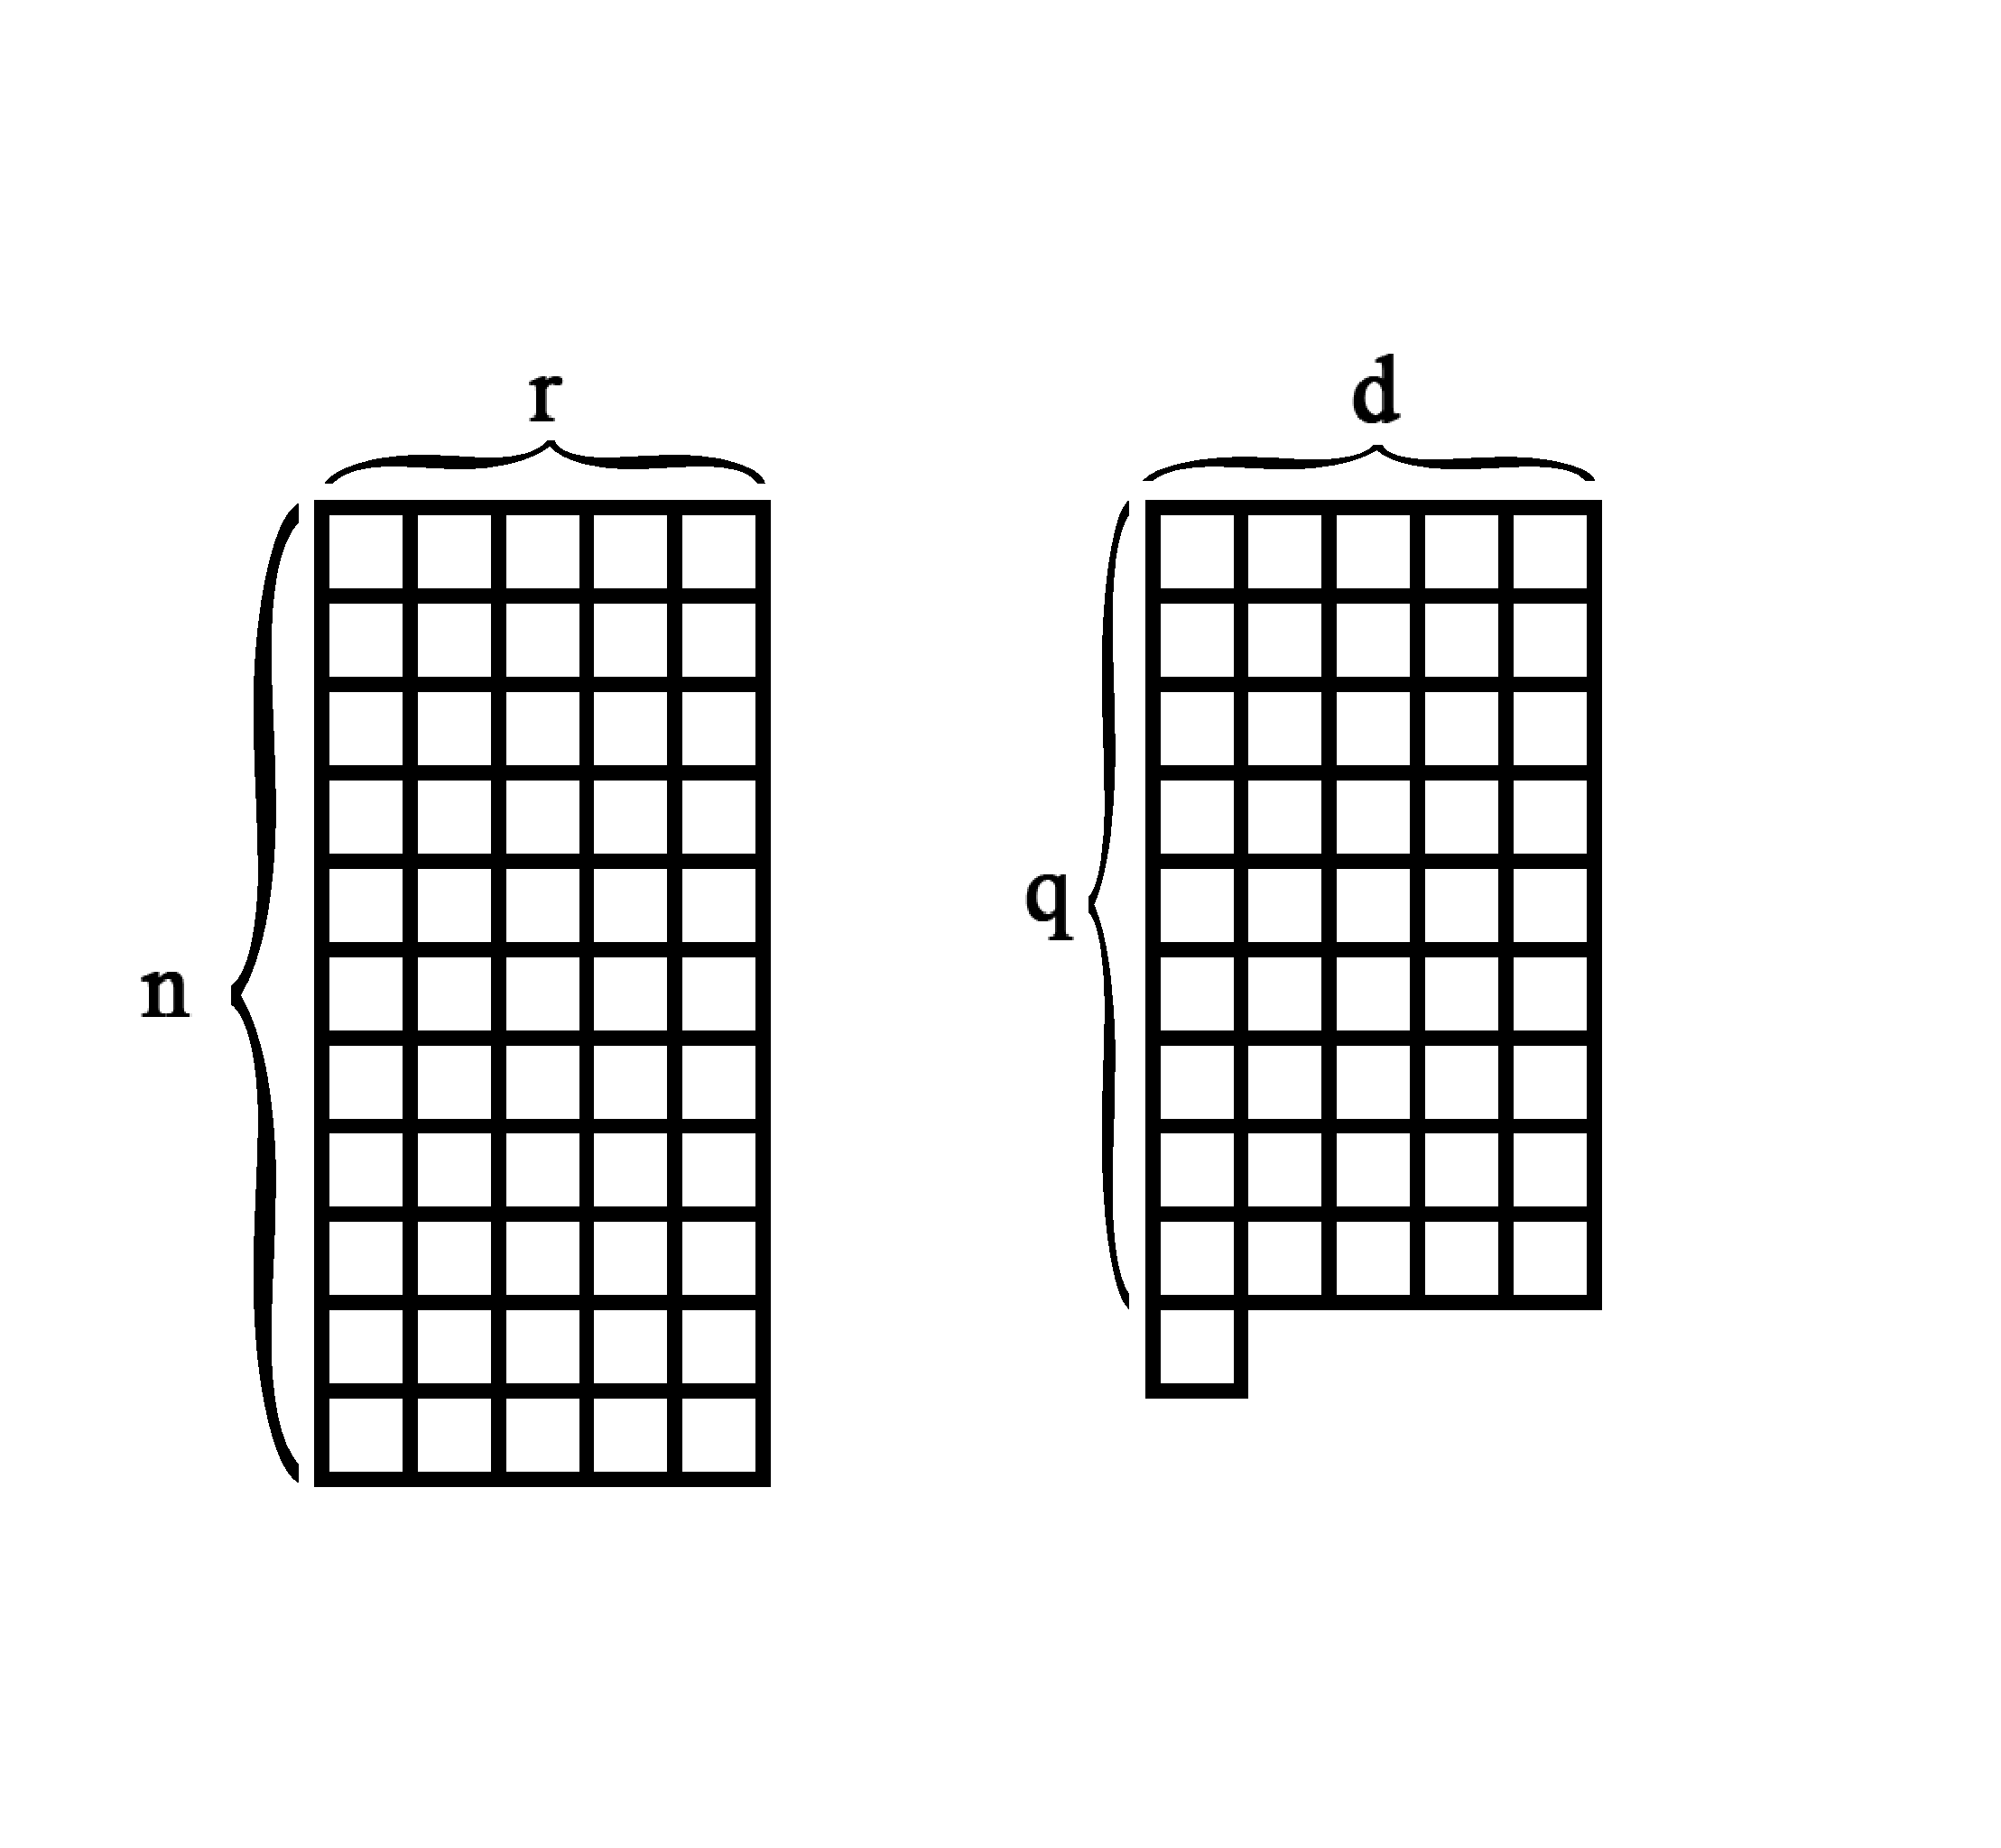
\includegraphics[width=0.4\textwidth]{figs/Young_diagrams.pdf}%
    }{%
        \fbox{\rule{0pt}{2in}\rule{0.7\textwidth}{0pt}}
    }
    \caption{Young diagrams of the representation $S_{\left(q+1, q^{d-1}\right)} V$ and the representation $\left(S_{\left(1^r\right)}V\right)^{\otimes n}$, where $n r=d q+1$.}
    \label{fig:Young_diagrams}
\end{figure}

\begin{smlemma}\label{lem:adjoint_in_end}
    $SU(d)$ representation $\operatorname{End}(V_{\omega_r})$, contains 
    exactly one copy of the adjoint and trivial representations.
\end{smlemma}

\begin{proof}
As in previous proof, we first work in the context of $GL_d(\mathbb{C})$ representations and then restrict ourselves to $SU(d)$ representations.
Since $\Lambda^r V \cong V_{\omega_r}$ as $SU(d)$ representations, it is reasonable to consider $\Lambda^r V \cong S_{\left(1^r\right)}(V)$ as $GL_d(\mathbb{C})$ representation.
First, notice that
$$
    \operatorname{End}(S_{\left(1^r\right)}(V))\cong S_{\left(1^r\right)}(V) \otimes (S_{\left(1^r\right)}(V))^* \cong (\det V)^{-1} \otimes S_{\left(1^r\right)} V \otimes S_{\left(1^{d-r}\right)} V.
$$
Now we apply Pieri's formula in the following form
\[
S_{\left(1^r\right)} V \otimes S_{\left(1^{d-r}\right)} V \cong \bigoplus_{i=0}^{\min (r, d-r)} S_{\left(2^i, 1^{d-2 i}\right)} V
\]
Indeed, starting from $(1^r)$ and multiplying by $(1^{d-r})$ we add a vertical strip of size $d-r$ to the first diagram (according to Pieri's formula). 
Since the first diagram is a single column itself, we have two options: add to an existing row, producing a row of length $2$, or
create a new row, producing a row of length $1$.
The resulting partition is 
$
\left(2^i, 1^{(r-i)+((d-r)-i)}\right)=\left(2^i, 1^{d-2 i}\right) .
$
Multiplicity representation, corresponding to each partition, is one -- again, according to Pieri's formula.
Thus,
\begin{equation}\label{eq:decompositionEnd}
    \operatorname{End}\left(S_{\left(1^r\right)}(V)\right) \cong \bigoplus_{i=0}^{\min (r, d-r)}(\operatorname{det} V)^{-1} \otimes S_{\left(2^i, 1^{d-2 i}\right)} V.
\end{equation}

Now let's find the expression of the adjoint representation as a polynomial $GL_d(\mathbb{C})$-module. On the one side, we have
\[
    \operatorname{End}(V)=V \otimes V^* \cong \mathbf{1} \oplus \mathrm{Ad}
\]
On the other side
\[
    V \otimes V^* \cong(\operatorname{det} V)^{-1} \otimes S_{\left(1\right)} V \otimes S_{\left(1^{d-1}\right)} V
\]
and using Pieri's formula again, we get
\[
    V \otimes V^* \cong (\operatorname{det} V)^{-1} \otimes \left(S_{\left(1^d\right)} V \oplus S_{\left(2,1^{d-2}\right)} V\right)=\mathbf{1} \oplus(\operatorname{det} V)^{-1} \otimes S_{\left(2,1^{d-2}\right)} V
\]
from which we derive
\[
    \mathrm{Ad} \cong(\operatorname{det} V)^{-1} \otimes S_{\left(2,1^{d-2}\right)} V
\]
and from decomposition (\ref{eq:decompositionEnd}) we conclude that
\[
    \operatorname{dim} \operatorname{Hom}_{GL_d(\mathbb{C})}\left(\mathrm{Ad}, \operatorname{End}\left(S_{\left(1^r\right)}(V)\right)\right)=1 .
\]
Finally, let's restrict ourselves to $SU(d)$ representations. To be precise, 
    \[
        S_{\left(1^r\right)}(V)\downarrow_{SU(d)}\cong V_{\omega_r}, \quad \mathrm{Ad}\downarrow_{SU(d)} \cong \mathrm{Ad},
    \]
From \ref{eq:decompositionEnd} we infer that there is exactly one copy of the trivial representation -- term $i=0$.
This completes our proof.
\end{proof}

We define generators of $\mathfrak{su}(d)$ (fundamental representation) in a standard way:
choose $t_a$ that are traceless Hermitian complex $d \times d$ matrices, where:
\begin{equation}\label{eq:sudgenerators}
t_a t_b=\frac{1}{2 d} \delta_{a b} I_d+\frac{1}{2} \sum_{c=1}^{d^2-1}\left(i f_{a b c}+d_{a b c}\right) t_c
\end{equation}
where the $f$ are the structure constants and are antisymmetric in all indices, while the $d$-coefficients are symmetric in all indices.
As a consequence,
$$
\left[t_a, t_b\right]=i \sum_{c=1}^{d^2-1} f_{a b c} t_c, \quad \left\{t_a, t_b\right\}=\frac{1}{d} \delta_{a b} I_d+\sum_{c=1}^{d^2-1} d_{a b c} t_c.
$$
With this definition conventional normalizations are
\begin{equation}\label{eq:sudnormalisation}
\operatorname{Tr}\left(t_a t_b\right)=\frac{1}{2} \delta_{a b}, \quad \sum_{c, e=1}^{d^2-1} d_{a c e} d_{b c e}=\frac{d^2-4}{d} \delta_{a b}.
\end{equation}
We will also use the following identities, which can be easily derived from the definition of generators:
\begin{equation}\label{eq:sudidentities}
    \sum_{m, n=1}^{d^2-1}f_{a m n} f_{b m n}=d \delta_{a b}, \quad \sum_{m, n=1}^{d^2-1}f_{a m n} d_{b m n}=0 , \quad \sum_{m=1}^{d^2-1}d_{a m m}=0 .
\end{equation}

We denote by $\{T_a\}$ the set of operators on $V_{\omega_r}$ that are representation of generators $\{t_a\}$ of $\mathfrak{su}(d)$, omitting the index $r$ for brevity.
Notice that $T_a$ are also traceless Hermitian complex matrices.
We will later need the following normalization 
\begin{equation}\label{eq:sudnormalisation_2}
\operatorname{Tr}_{V_{\omega_r}}\left(T_a T_b\right)=\kappa_{\omega_r} \delta_{a b}, \quad \kappa_{\omega_r}=\frac{1}{2}\binom{d-2}{r-1}.
\end{equation}

\begin{smproposition}\label{prop:SUdcov}
    Let
    $
        \mathcal H_L=V_{\omega_1},\;
        \mathcal H_P=(V_{\omega_r})^{\otimes n}
    $
    and $nr\equiv 1\;(\operatorname{mod} d)$.
    Equip \(\mathcal H_L\) with the fundamental representation of
    \(\mathfrak{su}(d)\), and equip \(\mathcal H_P\) with the transversal
    representation given by
    \begin{equation}
    \begin{gathered}
    t_a \rightarrow T_a \equiv \sum_{i=1}^n T_a^{(i)}, \quad a=1,\ldots,d^2-1
    \end{gathered}
    \end{equation}
    where $T_a^{(i)}$ is a representation of $t_a$ on the $i$-th physical space $V_{\omega_r}$, acting as in Eq.~\eqref{eq:action_on_extirior_power}.
    Then there exist a code space $\mathfrak{su}(d)$-covariant encoding $\mathcal{E}$ with respect to defined physical and logical representations, 
    such that the state seen by the environment after erasure of any single physical qudit is of the form   
    \[
        \rho^{(i)}\left(\rho_L\right)=\frac{I}{\operatorname{dim} V_{\omega_r}}+\frac{1}{n} \frac{1}{2\kappa_{\omega_r}} \sum_a r_a T_a^{(i)} .    
    \]
    Namely, this code space is one of the copies of the fundamental representation $V_{\omega_1}$ in $\left(V_{\omega_r}\right)^{\otimes n}$ 
    which is invariant under cyclic permutations of physical qudits.
\end{smproposition}

\begin{proof}
We recall that from Schur lemma $\left(V_{\omega_r}\right)^{\otimes n}\cong \bigoplus_{\lambda\in \Lambda} V_\lambda\otimes M_{\lambda}$, 
where $\Lambda$ is a set of irreducible representations of $SU(d)$, 
$V_\lambda$ is the irreducible representation space and $M_\lambda$ is the multiplicity space.

In Lemma~\ref{lem:fundamental_in_extirior_power} we prove that for the choice of individual physical space to be $V_{\omega_r}$ and $n r \equiv 1 (\bmod d)$, it is guaranteed 
that $\operatorname{dim} M_{V_{\omega_1}}>0$.

The linear extension $\Phi^{(i)}:\operatorname{End}(V_{\omega_1})\rightarrow \operatorname{End}(V_{\omega_r})$ of the reduced state map $\rho_L \rightarrow \rho^{(i)}\left(\rho_L\right)$ is an intertwiner of $SU(d)$ representations. 
Logical space as $SU(d)$ representation is
\[
     \text{End}(V_{\omega_1})\cong V_{\omega_1} \otimes (V_{\omega_1})^* \cong \mathbf{1} \oplus \mathrm{Ad}.
\]
For individual system representation $V_{\omega_r}$ we have the following decomposition
\[
    \text{End}(V_{\omega_r})\cong V_{\omega_r} \otimes V_{\omega_r}^* \cong \mathbf{1} \oplus \mathrm{Ad} \oplus \cdots.
\]
From Lemma~\ref{lem:adjoint_in_end} we infer that there is always exactly one copy of the trivial representation and also exactly one copy of the adjoint representation.
As an intertwiner $\Phi^{(i)}$ should have a form
\[
\Phi^{(i)}\cong I_{\mathbf{1}}\otimes A_{M_\mathbf{1}\rightarrow M_\mathbf{1}}\oplus I_{\mathrm{Ad}}\otimes A_{M_\mathrm{Ad}\rightarrow M_\mathrm{Ad}}
\]
and since $\dim M_\mathbf{1}=\dim M_\mathrm{Ad}=1$ we get
\begin{equation}
\begin{gathered}
        \Phi^{(i)}\left(\frac{I_d}{d}\right)=\frac{I_{V_{\omega_r}}}{\operatorname{dim} V_{\omega_r}},\\
        \Phi^{(i)}\left(\sum_a r_a t_a\right)=\beta^{(i)}\sum_a r_a T_a^{(i)}.
\end{gathered}
\end{equation}

Going back to reduced state map $\rho^{(i)}\left(\rho_L\right)$, since logical state has the following form
\[
     \rho_L=\frac{I_d}{d}+\left(\rho_L-\frac{I_d}{d}\right)=\frac{I_d}{d}+\sum_a r_a t_a,
\]
where $\frac{I}{d}$ is in trivial representation and $\rho_L-\frac{I}{d}$ is in adjoint representation, we have that $\rho^{(i)}\left(\rho_L\right)$ has the following form
\[
    \rho^{(i)}\left(\rho_L\right) = \frac{I_{V_{\omega_r}}}{\operatorname{dim} V_{\omega_r}}+\beta^{(i)} \sum_a r_a T_a^{(i)}.
\]
where $\beta^{(i)}$ is some constant that depends on the choice of code space.
Indeed, $\rho^{(i)}\left(\rho_L\right)$ is a covariant map, so it takes a trivial representation to a trivial representation and an adjoint representation.
And since we have chosen $V_{\omega_r}$ such that it contains exactly one copy of the adjoint representation, we have the desired form. Let

\[
    \mathcal{V}: V_{\omega_1} \rightarrow V_{\omega_r}^{\otimes n}
\]
our encoding isometry, where $V_{\omega_1}$ is the fundamental representation of $SU(d)$. 
We want to show

\[
\mathcal{V}^{\dagger} T_a^{(i)} \mathcal{V}=\alpha^{(i)} t_a.
\]
Equivalently, if we define
\begin{equation}\label{eq:Vt_aV}
     K_a^{(i)}:=\mathcal{V}^{\dagger} T_a^{(i)} \mathcal{V} \in \operatorname{End}\left(V_{\omega_1}\right),
\end{equation}
we need to show
\[
    K_a^{(i)}=\alpha^{(i)} t_a.
\]
From the fact that local generators transform in the adjoint representation, i. e.
\[
     \left(\bigotimes_{k=1}^n U^{(k)}(g)\right) T_a^{(i)} \left(\bigotimes_{k=1}^n U^{(k)}(g)\right)^{\dagger}=\sum_b \operatorname{Ad}_{b a}(g) T_a^{(i)}
\]
and the covariance condition of the encoding map we have
\[
     u(g) K_a^{(i)} u(g)^{\dagger}=\sum_b \operatorname{Ad}_{b a}(g) K_b^{(i)}.
\]
$\operatorname{End}\left(V_{\omega_1}\right)$ contains exactly one copy of adjoint representation
\[
     \operatorname{End}\left(V_{\omega_1}\right) \cong V_{\omega_1} \otimes V_{\omega_1}^* \cong \mathbf{1} \oplus \operatorname{Ad}
\]
which means that by Shur's lemma
\[
     \operatorname{dim} \operatorname{Hom}_{S U(d)}\left(\operatorname{Ad}, \operatorname{End}\left(V_{\omega_1}\right)\right)=1
\]
so we have that $K_a^{(i)}$ is proportional to $t_a$. Now we are to obtain $\beta^{(i)}$ in terms of $\alpha^{(i)}$. We have

\[
     \operatorname{Tr}\left(\rho^{(i)}\left(\rho_L\right) T_a^{(i)}\right)=\beta^{(i)} \sum_b r_b \operatorname{Tr}\left(T_b^{(i)} T_a^{(i)}\right) .
\]
From normalization relations~\eqref{eq:sudnormalisation} and~\eqref{eq:sudnormalisation_2} we get
\[
     \operatorname{Tr}\left(\rho^{(i)}\left(\rho_L\right) T_a^{(i)}\right)=\beta^{(i)} \kappa_{\omega_r} r_a .
\]
and on the other hand, using properties of $\Tr$ and covariance condition of encoding map we get
\[
     \operatorname{Tr}\left(\rho^{(i)}\left(\rho_L\right) T_a^{(i)}\right)=\operatorname{Tr}\left(\mathcal{V} \rho_L \mathcal{V}^{\dagger} T_a^{(i)}\right)=
     \operatorname{Tr}\left(\rho_L \mathcal{V}^{\dagger} T_a^{(i)} \mathcal{V}\right)=\alpha^{(i)} \operatorname{Tr}\left(\rho_L t_a\right) .
\]
from $\rho_L=\frac{I}{d}+\sum_a r_a t_a$, we have
$
     \operatorname{Tr}\left(\rho_L t_a\right)=\frac{1}{2} r_a
$
so on the other hand we have
$
     \operatorname{Tr}\left(\rho^{(i)}\left(\rho_L\right) T_a^{(i)}\right)=\frac{\alpha^{(i)}}{2} r_a .
$
from which we finally obtain the following expression for $\beta^{(i)}$:
\[
     \beta^{(i)}=\frac{1}{2\kappa_{\omega_r}}\alpha^{(i)}  .
\]

Finally, the reduced state on the $i$-th physical qudit has the following form
\[
    \rho^{(i)}\left(\rho_L\right)=\frac{I}{\operatorname{dim} V_{\omega_r}}+\alpha^{(i)} \frac{1}{2\kappa_{\omega_r}} \sum_a r_a T_a^{(i)} .
\]
Using the same code construction for symmetric code as we did for $SU(2)$ case (see the proof of the Proposition~\ref{prop:SU2cov}), namely, making code space invariant under cyclic shifts, 
our code space is such that $\alpha^{(i)}=\frac{1}{n}$ for all $i$, which gives the desired form of reduced state.

\end{proof}


\begin{smproposition}\label{prop:SUdcovfidelity}
    For the encoding $\mathcal{E}$ defined in the Proposition~\ref{prop:SUdcov} and noise channel $\mathcal{N}(\sigma)=\sum_{i=1}^n p_i \ket{i}\bra{i}_F \otimes \ket{e}\bra{e}_{A_i} \otimes \operatorname{Tr}_i(\sigma)$ the worst-case entanglement fidelity is
    \[
        F(\widehat{\mathcal{N} \circ \mathcal{E}}, \Lambda_0)=1-\frac{(d-1)^2(d+1)}{8 r(d-r)}\frac{1}{n^2}+O_{d}\left(n^{-3}\right),
    \]
    where we take $\Lambda_0(\rho)=\operatorname{Tr}(\rho)\omega_{\text{flag}}\otimes\frac{I_{V_{\omega_r}}}{\operatorname{dim} V_{\omega_r}}$, where $\omega_{\text {flag}}=\sum p_i|i\rangle\langle i|_{F_E}$.
\end{smproposition}

\begin{proof}
In this section, we will calculate the worst-case fidelity of $SU(d)$-covariant codes with flagged erasure error model
in the same way as we did for $SU(2)$-covariant codes. 
For the later calculations we will use notation $\beta:=\frac{1}{n} \frac{1}{2\kappa_{\omega_r}}$, $D=\operatorname{dim} V_{\omega_r}$.
Since reduced states are identical on each site, the complementary channel becomes
\[
        \widehat{\mathcal{N} \circ \mathcal{E}}(\rho)=\omega_{\text {flag }} \otimes \left(\frac{I_D}{D}+ \beta \sum_a r_a T_a^{(1)}\right),
\]
where $\omega_{\text {flag }}=\sum p_i|i\rangle\langle i|_{F_E}$ is the flag state. We chose the fixed channel to be 
$$
\Lambda_0(\rho)=\operatorname{Tr}(\rho)\cdot \omega_{\text {flag }}\otimes \frac{I_{D}}{D} \equiv \operatorname{Tr}(\rho)\cdot \omega_{\text {flag }}\otimes \tau.
$$ 
We drop flag state $\omega_{\text {flag }}$, since fidelity is invariant under 
tensor multiplication on the same state; we also omit the index of a site $(1)$.

As we know from \ref{fidelity_opt} the optimum of $F_{\rho}(\widehat{\mathcal{N} \circ \mathcal{E}}, \Lambda_0)$ 
is attained on the chaotic state $\frac{I_d}{d}$, its purification is maximally entangled state $\ket{\Psi}=\frac{1}{\sqrt{d}}\sum |r\rangle \otimes|r\rangle $. 
We have to compute $(\widehat{\mathcal{N} \circ \mathcal{E}} \otimes \mathrm{id})(\ket{\Psi}\bra{\Psi})$ and $(\Lambda_0 \otimes \mathrm{id})(\ket{\Psi}\bra{\Psi})$.
We define the linear extension of the reduced state channel to all complex matrices as follows
$$
\Phi: \operatorname{End}\left(V_{\omega_1}\right) \rightarrow \operatorname{End}\left(V_{\omega_r}\right), \quad \Phi\left(t_a\right):=T_a, \quad \Phi\left(\frac{I_d}{d}\right):=\tau
$$
and we will use the following notation for our derivations
\begin{equation}\label{eq:matr_units}
     E_{r s}:=|r\rangle\langle s|, \quad F_{r s}:=E_{r s}-\delta_{r s} \frac{I_d}{d}.
\end{equation}
For the constant channel, we have
\[
     \eta_{1/d}:=(\Lambda_0 \otimes \mathrm{Id})\left(\ket{\Psi}\bra{\Psi}\right)=\tau \otimes \frac{I_d}{d}.
\]  
For the complementary channel using 
$
\widehat{\mathcal{N} \circ \mathcal{E}}\left(E_{r s}\right)=\delta_{r s} \tau+\beta \Phi\left(F_{r s}\right) .
$
we define 
\[
\begin{gathered}
     \sigma_{1/d}:=\left(\widehat{\mathcal{N} \circ \mathcal{E}} \otimes \mathrm{Id}\right)\left(\ket{\Psi}\bra{\Psi}\right)=
     \frac{1}{d}\sum_{r, s=1}^d \widehat{\mathcal{N} \circ \mathcal{E}}\left(E_{r s}\right) \otimes|r\rangle\langle s| =\\
     =\frac{1}{d}\sum_{r, s=1}^d \left(\delta_{r s} \tau+\beta \Phi\left(F_{r s}\right)\right) \otimes|r\rangle\langle s| .
\end{gathered}
\]
We obtain the following expression for fidelity
\[
     f\left(\sigma_{1/d}, \eta_{1/d}\right)=\operatorname{Tr}\sqrt{\sqrt{\eta_{1/d}} \sigma_{1/d} \sqrt{\eta_{1/d}}}=\operatorname{Tr} \sqrt{\frac{1}{Dd^2}\left[\delta_{r s} \tau+\beta \Phi\left(F_{r s}\right)\right]_{r, s=1}^d}.
\]
Now, we recall that $\Phi$ actually acts as follows
\[
        \Phi\left(F_{a b}\right)=T_{a b}^{(r)}-\delta_{a b} \frac{r}{d} I_D,
\]
where $T_{a b}^{(r)}$ is the representation of $F_{a b}$ in the adjoint representation of $SU(d)$ and defined as follows
\[
    T_{a b}^{(r)}\left(v_1 \wedge \cdots \wedge v_r\right)=\sum_{m=1}^r v_1 \wedge \cdots \wedge E_{a b} v_m \wedge \cdots \wedge v_r
\]
so we can rewrite the expression for fidelity as follows
\[
\begin{aligned}
    f\left(\sigma_{1/d}, \eta_{1/d}\right)&=\operatorname{Tr} \sqrt{\frac{1}{Dd^2}\left[\delta_{a b} \tau+\beta \left(T_{a b}^{(r)}-
    \delta_{a b} \frac{r}{d} I_D\right)\right]_{a, b=1}^d}\\&\equiv\frac{1}{d \sqrt{D}} \operatorname{Tr} \sqrt{\frac{I_{D d}}{D}+\beta B} .
\end{aligned}
\]
where 
\[
    B=\left(\begin{array}{cccc}
    T_{11}^{(r)}-\frac{r}{d} I_D & T_{12}^{(r)} & \cdots & T_{1 d}^{(r)} \\
    T_{21}^{(r)} & T_{22}^{(r)}-\frac{r}{d} I_D & \cdots & T_{2 d}^{(r)} \\
    \vdots & \vdots & \ddots & \vdots \\
    T_{d 1}^{(r)} & T_{d 2}^{(r)} & \cdots & T_{d d}^{(r)}-\frac{r}{d} I_D
    \end{array}\right).
\]
We are now to expand this expression up to a leading order in $\beta$
\[
\begin{aligned}
        f\left(\sigma_{1/d}, \eta_{1/d}\right)&=1+\frac{\beta}{2 d} \operatorname{Tr} B-\frac{D \beta^2}{8 d} \operatorname{Tr} B^2+O_{d}\left(\beta^3\right)
        \\&=1-\frac{D^2 \beta^2}{8 d}\left(r(d-r+1)-\frac{r^2}{d}\right)+O_{d}\left(\beta^3\right)
\end{aligned}
\]
where we use the fact that $\operatorname{Tr} B=0$ and $\operatorname{Tr} B^2=D\left(r(d-r+1)-\frac{r^2}{d}\right)$. Indeed, 
$$
\begin{aligned}
    \operatorname{Tr} B^2&=\sum_{a, b=1}^d \operatorname{Tr}_{V_{\omega_r}}\left(\Phi\left(F_{a b}\right) \Phi\left(F_{b a}\right)\right)=\sum_{a\neq b}^d\operatorname{Tr}\left(T_{a b}^{(r)} T_{b a}^{(r)}\right)+\sum_{a=1}^d \operatorname{Tr}\left(T_{a a}^{(r)}-\frac{r}{d} I_D\right)^2\\&=d(d-1)\binom{d-2}{r-1}+d\frac{Dr(d-r)}{d^2}=D\left(r(d-r+1)-\frac{r^2}{d}\right)
\end{aligned}
$$
Finally, if we substitute $\beta=\frac{1}{n} \frac{1}{2\kappa_{\omega_r}}$, $D=\operatorname{dim} V_{\omega_r}$ and 
$\kappa_{\omega_r}=\frac{1}{2}\binom{d-2}{r-1}$ into $F(\widehat{\mathcal{N} \circ \mathcal{E}}, \Lambda_0)=f(\sigma_{1/d}, \eta_{1/d
})$ we get a desired expression for fidelity.
\end{proof}

\subsection{Explicit Decoder construction}\label{subsec:supple_decoder}

In this section, we will construct an explicit decoder for $SU(d)$-covariant codes with the erasure error model.
For this, we will use the Petz recovery map, which is defined as follows
\begin{smdefinition}
    For a given channel $\mathcal{N}$ and reference state $\omega$, the Petz map $\mathcal{P}_{\omega, \mathcal{N}}$ is defined as:
    \[
        \mathcal{P}_{\omega, \mathcal{N}}(\sigma)=\omega^{1 / 2} \mathcal{N}^*\left(\mathcal{N}(\omega)^{-1 / 2} \sigma \mathcal{N}(\omega)^{-1 / 2}\right) \omega^{1 / 2},
    \]
    where $\mathcal{N}^*$ is the adjoint of $\mathcal{N}$ with respect to the Hilbert-Schmidt inner product, and $\omega$ is so-called reference state.
\end{smdefinition}

\begin{smtheorem}\label{thm:petz_decoder_explicit}
For the encoding $\mathcal E$ and the flagged single-qudit erasure channel $\mathcal N$ defined in Theorem~\ref{thrm:sudscale}, 
the Petz recovery map with reference state $\omega=I_d/d$ has the form
$$
\mathcal R_{\mathrm{Petz}}(X)
=
\sum_{i:,p_i>0}
\mathcal{V}^\dagger
\left(
S_i^{-1/2}
\langle i,e|X|i,e\rangle_{F,A_i}
S_i^{-1/2}
\otimes I_{A_i}
\right)
\mathcal{V},
$$
where $\mathcal{V}$ is the encoding isometry and
$$
S_i
:=
\operatorname{Tr}_i\left(\mathcal{V}\mathcal{V}^\dagger\right).
$$
Moreover, this recovery is near-optimal in the sense that
$$
    d\left(
    \mathcal R_{\mathrm{Petz}}
    \circ
    \mathcal N
    \circ
    \mathcal E,
    \mathrm{id}
    \right)
    =
    O_{d}(n^{-1}) .
$$
\end{smtheorem}

\begin{proof}
Define the erased channel for site $i$ by
$
    \mathcal{C}_i\left(\rho_L\right):=\operatorname{Tr}_{i}\left(\mathcal{V} \rho_L \mathcal{V}^{\dagger}\right).
$
Our noise channel in this notation can be written as
$
    \mathcal{N}(\sigma)=\sum_{i=1}^n p_i\ket{i}\bra{i}_F \otimes \ket{e}\bra{e}_{A_i}\otimes \mathcal{C}_i.
$
We take a reference state $\omega$ to be the chaotic state $\frac{I}{d}$, which is the only $SU(d)$-invariant state on logical space. We get
\[
    \mathcal{C}_i\left(\omega\right)=\frac{1}{d} \operatorname{Tr}_i\left(\mathcal{V} \mathcal{V}^{\dagger}\right)=\frac{S_i}{d},
\]
where we defined $S_i:=\operatorname{Tr}_i\left(\mathcal{V} \mathcal{V}^{\dagger}\right)$. One can easily check that
\[
    \mathcal{C}_i^{\dagger}(Y)=\mathcal{V}^{\dagger}\left(Y \otimes I_{W_i}\right) \mathcal{V}
\]
where we denoted $W_i$ as the Hilbert space associated with site $i$. Thus, the recovery map is given by
\[
    \mathcal{R}_{\mathrm{Petz}}(X)=\sum_{i: p_i>0} \mathcal{V}^{\dagger}\left(S_i^{-1 / 2} \langle i, e| X|i,e\rangle_{F, A_i} S_i^{-1 / 2} \otimes I_{W_i}\right) \mathcal{V},
\]
where the inverse should always be understood as the inverse on the support of $S_i$. Now, let's explore the performance of this decoder, 
i. e. find $F\left(\mathcal{R}_{\mathrm{Petz}} \circ \mathcal{N}\circ \mathcal{E}, \mathrm{id}\right)$, since we 
are in AQECC setting. We denote
\[
    \Phi:=\mathcal{R}_{\mathrm{Petz}} \circ \mathcal{N}\circ \mathcal{E}
\]
and let's analyze the structure of $\Phi$. First of all, $\Phi: \operatorname{End}(\mathcal{H}_L)\rightarrow \operatorname{End}(\mathcal{H}_L)$ is a 
$SU(d)$-covariant map, i. e.
\[
    \Phi\left(u(g) \rho u(g)^{\dagger}\right)=u(g) \Phi(\rho) u(g)^{\dagger}, \quad \forall g \in SU(d).
\]
Indeed, $\mathcal{C}_i\left(u(g) \rho u(g)^{\dagger}\right)=U^{\hat{i}}(g) \mathcal{C}_i(\rho) \left(U^{\hat{i}}(g)\right)^{\dagger}$ and $S_i^{-1 / 2}$ 
commutes with $U^{\hat{i}}(g)$ on the support of $S_i$. So it has to take the following form
\[
    \Phi(\rho)=\lambda_{\mathrm{Petz}} \rho+\left(1-\lambda_{\mathrm{Petz}}\right) \frac{I_d}{d} \operatorname{Tr} \rho,
\]
that is basically a depolarizing channel with depolarizing parameter $\lambda_{\mathrm{Petz}}$. Let's show that this depolarizing parameter is given by
\begin{equation}\label{eq:lambdaPetz}
    \lambda_{\text{Petz}}=\frac{2}{d^2-1}\sum_{i=1}^n p_i \sum_{a=1}^{d^2-1} \operatorname{Tr}\left[S_i^{-1 / 2} \mathcal{C}_i\left(t_a\right) 
    S_i^{-1 / 2} \mathcal{C}_i\left(t_a\right)\right] .
\end{equation}
Indeed, since $\Phi\left(t_a\right)=\lambda_{\text{Petz}} t_a$, we have
$$
\operatorname{Tr}\left(t_a \Phi\left(t_a\right)\right)=\frac{1}{2} \lambda_{\text{Petz}},
$$
where we used $\operatorname{Tr}\left(t_a t_b\right)=\frac{1}{2} \delta^{a b}$. Summing over $a$,
$$
\lambda_{\text{Petz}}=\frac{2}{\left(d^2-1\right)} \sum_{a=1}^{d^2-1} \operatorname{Tr}\left(t_a \Phi\left(t_a\right)\right)
$$
Now substitute the Petz formula:
$$
\Phi_{\mathrm{Petz}}\left(t_a\right)=\sum_i p_i \mathcal{V}^{\dagger}\left(S_i^{-1 / 2} \mathcal{C}_i\left(t_a\right) S_i^{-1 / 2} \otimes I_{A_i}\right) \mathcal{V}.
$$
Hence
$$
\operatorname{Tr}\left(t_a \Phi_{\text{Petz}}\left(t_a\right)\right)=\sum_i p_i \operatorname{Tr}\left[S_i^{-1 / 2} 
\mathcal{C}_i\left(t_a\right) S_i^{-1 / 2} \mathcal{C}_i\left(t_a\right)\right]
$$
where we used the partial-trace identity
$
\operatorname{Tr}\left(X\left(Y \otimes I_W\right)\right)=\operatorname{Tr}\left(\operatorname{Tr}_W(X) Y\right),
$
with $X=\mathcal{V} t^a \mathcal{V}^{\dagger}$ and $Y=A^{-1 / 2} \mathcal{C}_i\left(t^a\right) A^{-1 / 2}$, gives desired expression for $\lambda_{\mathrm{Petz}}$.

For a pure state \(\psi=|\psi\rangle\langle\psi|\), we have \(\Phi_{\mathrm{Petz}}(\psi)=\lambda_{\mathrm{Petz}}\psi+(1-\lambda_{\mathrm{Petz}})I_d/d\). 
Since the target state is pure, the root fidelity is
\[
f(\Phi_{\mathrm{Petz}}(\psi),\psi)
=
\sqrt{\langle\psi|\Phi_{\mathrm{Petz}}(\psi)|\psi\rangle}
=
\sqrt{\lambda_{\mathrm{Petz}}+\frac{1-\lambda_{\mathrm{Petz}}}{d}} .
\]
This expression is independent of \(\psi\). Hence
\[
\eta_{\mathrm{Petz}}^{\mathrm{st}}
:=
1-\min_{\psi}f^2(\Phi_{\mathrm{Petz}}(\psi),\psi)
=
\frac{d-1}{d}(1-\lambda_{\mathrm{Petz}}).
\]

Our channel fidelity is defined as the minimum over \(\rho\) of \(F_\rho(\Phi_{\mathrm{Petz}},\mathrm{id})=f((\Phi_{\mathrm{Petz}}\otimes\mathrm{id})(|\psi_\rho\rangle\langle\psi_\rho|),|\psi_\rho\rangle\langle\psi_\rho|)\), where \(|\psi_\rho\rangle\) purifies \(\rho\). 
For the depolarizing channel \(\Phi_{\mathrm{Petz}}\), one finds
\[
(\Phi_{\mathrm{Petz}}\otimes \mathrm{id})(|\psi_\rho\rangle\langle\psi_\rho|)
=
\lambda_{\mathrm{Petz}}|\psi_\rho\rangle\langle\psi_\rho|
+(1-\lambda_{\mathrm{Petz}})\frac{I_d}{d}\otimes \rho_R .
\]
Since the target is pure, this gives \(F_\rho(\Phi_{\mathrm{Petz}},\mathrm{id})=\sqrt{\lambda_{\mathrm{Petz}}+\frac{1-\lambda_{\mathrm{Petz}}}{d}\operatorname{Tr}(\rho^2)}\). 
This quantity is minimized at \(\rho=I_d/d\), i.e. when \(\operatorname{Tr}(\rho^2)=1/d\). Therefore
\[
F(\Phi_{\mathrm{Petz}},\mathrm{id})
=
\sqrt{\lambda_{\mathrm{Petz}}+\frac{1-\lambda_{\mathrm{Petz}}}{d^2}} .
\]
Equivalently,
\[
\eta_{\mathrm{Petz}}^{\mathrm{ent}}
:=
1-F^2(\Phi_{\mathrm{Petz}},\mathrm{id})
=
\frac{d^2-1}{d^2}(1-\lambda_{\mathrm{Petz}})
=
\frac{d+1}{d}\eta_{\mathrm{Petz}}^{\mathrm{st}} .
\]

Thus, the exact worst-case channel fidelity of the Petz-recovered channel is determined by \(\lambda_{\mathrm{Petz}}\). 
However, analyzing this expression directly would require obtaining the scaling of \(\lambda_{\mathrm{Petz}}\) in terms of \(n\). 
This, in turn, requires a careful analysis of Eq.~\eqref{eq:lambdaPetz}, namely of the scaling of \(A\) and \(\mathcal C_i(\bar t_a)\) with \(n\). 
This is highly nontrivial, because these operators lie in the adjoint representation inside \((V_{\omega_r})^{\otimes(n-1)}\), 
where the adjoint component appears with large multiplicity, in contrast to the single-qudit case. 
Similar complications will appear below in the analysis of multi-qudit erasure errors.

We leave a direct analysis of \(\lambda_{\mathrm{Petz}}\) for future work. In this work we use the near-optimality theorem of Ng and Mandayam for the transpose channel, 
equivalently the Petz recovery map with the maximally mixed code state as reference state~\cite{Ng2010}. Their result states that
\[
\eta_{\mathrm{Petz}}^{\mathrm{st}}
\le
\eta_{\mathrm{op}}^{\mathrm{st}}
\frac{(d+1)-\eta_{\mathrm{op}}^{\mathrm{st}}}
{1+(d-1)\eta_{\mathrm{op}}^{\mathrm{st}}},
\]
where \(\eta_{\mathrm{op}}^{\mathrm{st}}:=\min_{\mathcal R}[1-\min_{\psi}f^2(\psi,(\mathcal R\circ\mathcal C)(\psi))]\). 
Moreover, the optimal state-fidelity error is bounded by the optimal entanglement-fidelity error, \(\eta_{\mathrm{op}}^{\mathrm{st}}\leq \eta_{\mathrm{op}}^{\mathrm{ent}}\). 
Therefore, since Theorem~$2$ from the main part of the paper gives \(\eta_{\mathrm{op}}^{\mathrm{ent}}=O_{d}(n^{-2})\), we obtain \(\eta_{\mathrm{Petz}}^{\mathrm{st}}=O_{d}(n^{-2})\). 
Finally, using \(\eta_{\mathrm{Petz}}^{\mathrm{ent}}=\frac{d+1}{d}\eta_{\mathrm{Petz}}^{\mathrm{st}}\), we conclude that
\[
\eta_{\mathrm{Petz}}^{\mathrm{ent}}=O_{d}(n^{-2}).
\]
This gives the desired scaling.

\end{proof}

\subsection{Flagged two- and three-qudit erasure}\label{subsec:supple_multi_erasure_noise}

The following Lemmas~\ref{lem:M_module_irreducibility}-\ref{lem:3-body_action} are axiliary results that we will need for our analysis of multi-qudit 
erasure errors and thus can be skipped on first reading.
For notation see Section~\ref{sec:supple_sud} and Nomenclature section.

\begin{smlemma}\label{lem:M_module_irreducibility}
    Let $M_{\omega_1}$ be a multiplicity space of the fundamental $SU(d)$ representation $V_{\omega_1}$ in $\left(V_{\omega_1}\right)^{\otimes n}$, where $n\equiv 1 \pmod{d}$. 
    Then $M_{\omega_1}$ is an irreducible $S_n$-module, namely the Specht module $[q+1, q^{d-1}]$, where $q=\frac{n-1}{d}$.
\end{smlemma}

\begin{proof}
    We recall the notation $\mathcal{V}=\C^d$. As always, we first work in the context of $GL_d(\mathbb{C})$ representations and then restrict ourselves to $SU(d)$ representations. 
    From the Schur-Weil duality, we have the following decomposition
    \[
        V^{\otimes n} \cong \bigoplus_{\lambda \vdash n, \ell(\lambda) \leq d} S_\lambda(V) \otimes[\lambda],
    \]
    where $S_\lambda(V)$ is $GL_d(\mathbb{C})$-module and $[\lambda]$ is irreducible $S_n$-module, known as Specht module.
    If we restrict this decomposition to $SU(d)$, then we get
    \[
        V^{\otimes n}\downarrow_{SU(d)}\cong V_{\omega_1}^{\otimes n} \cong \bigoplus_{\lambda \vdash n, \ell(\lambda) \leq d}\left(S_\lambda(V) \downarrow_{S U(d)}\right) \otimes[\lambda],
    \]
    where $S_\lambda(V) \downarrow_{S U(d)}$ is the restriction of $GL_d(\mathbb{C})$-module $S_\lambda(V)$ to $SU(d)$. 
    The decomposition is basically the same as for $GL_d(\mathbb{C})$ case, but the main difference
    is that $S_\lambda(V) \downarrow_{S U(d)}$ may coincide with $S_\mu(V) \downarrow_{S U(d)}$ for $\lambda \neq \mu$, 
    so multiplicity of $V_{\omega_1}$ as a representation of $SU(d)$ requires a careful analysis.
    Multiplicity space $M_{\omega_1}$ is described by the following formula
    \[
        M_{\omega_1}\cong \operatorname{Hom}_{S U(d)}\left(V_{\omega_1}, V_{\omega_1}^{\otimes n}\right) 
        \cong \bigoplus_{\lambda \vdash n, \ell(\lambda) \leq d} \operatorname{Hom}_{S U(d)}\left(V_{\omega_1}, S_\lambda(V) \downarrow_{S U(d)}\right) \otimes[\lambda],
    \]
    so we can write the following
    \[
        M_{\omega_1} \cong \bigoplus_{\lambda \vdash n, \ell(\lambda) \leq d} m_\lambda[\lambda],
    \]
    where since $S_\lambda(V)$ is still irreducible as a representation of $SU(d)$, we have $m_{\lambda}\in \{0,1\}$ for every
    $\lambda$.
    The restriction $S_\lambda(V)\downarrow_{SU(d)}$ is indeed irreducible. By the unitarian trick, $S_\lambda(V)$ is irreducible as a representation 
    of the compact group $U(d)$, because $\mathfrak{gl}_d(\C)$ is the complexification of $\mathfrak u(d)$ and the two therefore have the same invariant subspaces. 
    Every element of $U(d)$ is the product of an element of $SU(d)$ with a central phase $e^{i\theta}I$, and the latter acts on $S_\lambda(V)\subseteq V^{\otimes|\lambda|}$ 
    by the scalar $e^{i|\lambda|\theta}$. A subspace invariant under $SU(d)$ is therefore invariant under all of $U(d)$, hence is $0$ or $S_\lambda(V)$. 
    Irreducibility of the restriction then makes $\operatorname{Hom}_{SU(d)}(V_{\omega_1},S_\lambda(V)\downarrow_{SU(d)})$ one-dimensional when $S_\lambda(V)\downarrow_{SU(d)}\cong V_{\omega_1}$, and zero otherwise.
    We need to show that $m_\lambda=1$ for exactly one $\lambda$. Indeed,
    $S_\lambda(V) \downarrow_{S U(d)} \cong V_{\omega_1}$ happens exactly iff $\lambda=\left(q+1, q^{d-1}\right)$ for some $q\geq 0$.
    Since also $|\lambda|=n$, we have $n=(q+1)+q(d-1)=d q+1$, so $q=\frac{n-1}{d}$ is an integer. 
    Therefore,
    \[
        M_{\omega_1} \cong\left[q+1, q^{d-1}\right],
    \]
    which proves the lemma.
\end{proof}

\begin{smlemma}\label{lem:dimension_formula}
    Let $[q+1, q^{d-1}]$ be the Specht module corresponding to the partition $(q+1, q^{d-1})$. Then
    \[
        \operatorname{dim} [q+1, q^{d-1}] = \frac{(d q+1)!d!\prod_{i=0}^{d-2} i!}{(q+d)!\prod_{i=0}^{d-2}(q+i)!}.
    \]
\end{smlemma}

\begin{proof}
    The general formula for the dimension of Specht module $[\lambda]$ corresponding to the partition $\lambda$ is given by the hook-length formula, i. e.
    \[
        \operatorname{dim} [\lambda] = \frac{n!}{\prod_{(i, j) \in \lambda} h_{i j}} .
    \]
    where $h_{ij}$ is the hook length of the box in the $i$-th row and $j$-th column, precisely
    \[
        h_{i j}=\#\{\text { boxes to the right of }(i, j)\}+\#\{\text { boxes below }(i, j)\}+1 .
    \]
    It can also be expressed as
    $
        h_{i j}=\lambda_i-j+\lambda_j^{\prime}-i+1 .
    $
    Our Young diagram has the shape of a rectangle with an extra box in the top right corner, and its transpose 
    has the shape of a rectangle with an extra box in the bottom left corner, i. e.
    $$
        \lambda=(q+1, \underbrace{q, \ldots, q}_{d-1 \text { times }}), \quad \lambda'=(\underbrace{d, d, \ldots, d}_{q \text { times }}, 1).
    $$
    Now let's compute the hook lengths for each box in the Young diagram $\lambda$ -- row by row.
    First row, columns $1 \leq j \leq q$. Here $\lambda_1 = q+1$ and $\lambda_j'=d$, 
    $
        h_{1 j}=(q+1-j)+(d-1)+1=q+d+1-j.
    $
    The extra box in the first row has length 1, i. e. 
    $
        h_{1, q+1}=1.
    $
    Thus, their product is
    \[
        \prod_{j=1}^q h_{1 j}=\prod_{j=1}^q(q+d+1-j)=\frac{(q+d)!}{d!} .
    \]
    Rows $2 \leq i \leq d$, columns $1 \leq j \leq q$. Here $\lambda_i=q$ and $\lambda_j'=d$, so
    $
        h_{i j}=(q-j)+(d-i)+1=q+d-i-j+1 .
    $
    Thus, their product is
    \[
       \prod_{i=2}^d \prod_{j=1}^q h_{i j}=\frac{(q+d-i)!}{(d-i)!}.
    \]
    Combining all together, we have
    \[
        \prod_{(i, j) \in \lambda} h_{i j}=\frac{(q+d)!}{d!} \prod_{i=2}^d \frac{(q+d-i)!}{(d-i)!}
    \]
    and the formula in the formulation of the Lemma follows immediately.

\end{proof}

\begin{smlemma}\label{lem:dimension_bound}

Let $[q+1, q^{d-1}]$ be the Specht module corresponding to the partition $(q+1, q^{d-1})$. 
Then, for $q\geq d$ the following lower bound holds
\[
    \operatorname{dim} [q+1, q^{d-1}] \geq \left(\frac{d!\sqrt{2 \pi d}\prod_{i=0}^{d-2} i!}{e^d 2^{\frac{d^2-d+2}{2}}} \right) d^{d q} q^{-\frac{d^2+1}{2}} := C_d d^{d q} q^{-\frac{d^2+1}{2}}.
\]

\end{smlemma}

\begin{proof}
    From the previous lemma, we have
\[
    \operatorname{dim} [q+1, q^{d-1}]=\frac{(d q+1)!d!\prod_{i=0}^{d-2} i!}{(q+d)!\prod_{i=0}^{d-2}(q+i)!}
\]
and we need to estimate this quantity from below. Using obvious bounds
\[
    (q+d)!\leq q!(q+d)^d, \quad(q+i)!\leq q!(q+d)^i \quad(0 \leq i \leq d-2),
\]
we can express the denominator as
\[
    (q+d)!\prod_{i=0}^{d-2}(q+i)!\leq(q!)^d(q+d)^{\frac{d^2-d+2}{2}},
\]
so we have
\begin{equation}\label{eq:specht_dim_lb}
    \operatorname{dim} [q+1, q^{d-1}] \geq d!\prod_{i=0}^{d-2} i! \cdot \frac{(dq)!}{(q!)^d(q+d)^{\frac{d^2-d+2}{2}}}.
\end{equation}
Notice, that we are interested in scaling of $\operatorname{dim} [q+1, q^{d-1}]$ as $q$ grows, because in our setting
$d$ is fixed and $q$ depends linearly on $n$ (recall that $n=d q+1$). Using a simplified version of Robbins' bounds 
(which are derived from famous Stirling's formula, see~\cite{Robbins1955}), we get 
\[
   \sqrt{2 \pi N}(N / e)^N \leq \sqrt{2 \pi n}\left(\frac{n}{e}\right)^n e^{\frac{1}{12 n+1}} 
   \leq N!\leq \sqrt{2 \pi n}\left(\frac{n}{e}\right)^n e^{\frac{1}{12 n}} \leq e \sqrt{N}(N / e)^N.
\]
Then
\[
    \frac{(d q)!}{(q!)^d} \geq \frac{\sqrt{2 \pi d q}(d q / e)^{d q}}{\left(e \sqrt{q}(q / e)^q\right)^d}=\frac{\sqrt{2 \pi d}}{e^d} d^{d q} q^{-(d-1) / 2}
\]
Substituting into lower bound~\eqref{eq:specht_dim_lb} we get
\[
    \operatorname{dim} [q+1, q^{d-1}] \geq d!\prod_{i=0}^{d-2} i! \cdot \frac{\sqrt{2 \pi d}}{e^d} d^{d q} q^{-(d-1) / 2}(q+d)^{-\frac{d^2-d+2}{2}} 
    \geq \left(\frac{d!\sqrt{2 \pi d}\prod_{i=0}^{d-2} i!}{e^d 2^{\frac{d^2-d+2}{2}}} \right) d^{d q} q^{-\frac{d^2+1}{2}},
\]
where we used the condition $q\geq d$ in the second inequality. This completes our proof.

\end{proof}

The following lemma was proven in~\cite{LarsenShalev2008}. We will need it as a tool for bounding characters in Lemmas~\ref{lem:2_transitive_subgroup} and~\ref{lem:3_transitive_subgroup}.

\begin{smlemma}\label{lem:character_bound}
    Let $\sigma \in S_n$ and $\chi \in \text{Irr}(S_n)$. If $\sigma$ is fixed-point-free, or has $n^{o(1)}$ fixed points, then
    \[
        |\chi(\sigma)| \leq \chi(1)^{1 / 2+o(1)}.
    \]
\end{smlemma}

\begin{smlemma} \label{lem:2_transitive_subgroup}
    There exists infinitely many primes $p$ such that $n$ is a prime power, i. e. $n=p^k$ for any $k\geq 1$, and $n\equiv 1 \pmod{d}$, there is a family of $2$-transitive subgroups of $S_n$, namely
    \begin{equation}\label{eq:AGL}
        G\equiv\operatorname{AGL}(1, n)=\left\{x \mapsto a x+b: a \in \mathbb{F}_n^{\times}, b \in \mathbb{F}_n\right\}\leq S_n,
    \end{equation}
    acting on $\mathbb{F}_n$, such that for sufficiently large $q:=\frac{n-1}{d}$ (i. e. for sufficiently large $n$), we have 
    \[\dim [q+1, q^{d-1}]^G > 0.\]
\end{smlemma}

\begin{smremark} \label{rem:infinitely_many_primes}
    First of all, $n$ has to be a prime power, since $n$ is the size of the field $\mathbb{F}_{n}$. 
    The fact that an infinite family of such $p$ (i.e., infinitely many $p$ such that $n=p^k$ for any $k\geq 1$, and $n\equiv 1 \pmod{d}$) exists is a direct consequence of one of Dirichlet's 
    Theorems on Arithmetic Progressions.
    Indeed, the theorem directly states that there are infinitely many primes $p$ such that $p \equiv 1 \pmod{d}$.
    To provide proof for arbitrary $k\geq 1$, we write $p=1+d q$ for some $q\geq 1$, and then we have
    \[
        p^k=(1+d q)^k=\sum_{j=0}^k\binom{k}{j}(d q)^j=1+\sum_{j=1}^k\binom{k}{j}(d q)^j := 1+d \cdot t,
    \]
    thereby $p^k \equiv 1 \pmod{d}$ for any $k\geq 1$.
\end{smremark}

\begin{proof}
The fact that given $G$ is $2$-transitive is easy to see. Indeed, given any two pairs of distinct elements $(x, y)$ and $(x', y')$ in $\mathbb{F}_n$, we can do the following mapping
\[
    z \mapsto a z+b, \quad a=\frac{y^{\prime}-x^{\prime}}{y-x}, \quad b=x^{\prime}-a x
\]
that sends $(x, y)$ to $(x', y')$, so it is $2$-transitive.

Now we need to show that $\dim [q+1, q^{d-1}]^G > 0$. For that, we recall the following formula from the character theory of finite groups:
\[
    \operatorname{dim}\left([\lambda]\right)^G=\frac{1}{|G|} \sum_{g \in G} \chi^\lambda(g)=\frac{1}{|G|}\left(\chi^\lambda(1)+\sum_{g \neq 1}\chi^\lambda(g) \right),
\]
so proving that $\dim [q+1, q^{d-1}]^G > 0$ is equivalent to proving that
\[
    \sum_{1 \neq g \in G}\left|\chi^\lambda(g)\right|<\chi^\lambda(1).
\]
Now we are to apply the bound from Lemma \ref{lem:character_bound}. Let's
prove that every non-identity element of $G$ has at most $1$ fixed point (which is definitely $n^{o(1)}$ fixed points).
Consider $g\neq 1 \in G$, the general form would be $x \mapsto a x+b, \quad a \in \mathbb{F}_n^{\times}, b \in \mathbb{F}_n$. 
If $a=1$, then $g$ is a translation, and it has no fixed points. If $a \neq 1$, then the fixed-point equation $x=a x+b$ has exactly one solution $x=\frac{b}{1-a}$, so $g$ has exactly one fixed point.
Therefore, we can apply the bound from Lemma \ref{lem:character_bound}, and we have
\[
    \left|\chi^\lambda(g)\right| \leq\left(\chi^\lambda(1)\right)^{1 / 2+\varepsilon_n} \quad(1 \neq g \in G) .
\]
where $\varepsilon_n \to 0$ as $n \to \infty$. Group $G$ size can be estimated as follows
$
    |G|=n(n-1)<n^2 .
$
Combining these two inequalities we have
\[
    \sum_{1 \neq g \in G}\left|\chi^\lambda(g)\right| \leq(|G|-1)\left(\chi^\lambda(1)\right)^{1 / 2+\varepsilon_n}<n^2\left(\chi^\lambda(1)\right)^{1 / 2+\varepsilon_n} .
\]
We choose $n$ sufficiently large, we can make $\varepsilon_n<\frac{1}{3}$, and recalling exponential scaling with $n$ 
of $\chi^{\lambda}(1)$ from Lemma~\ref{lem:dimension_bound}, i. e. $\dim \left[q+1, q^{d-1}\right]= \chi^\lambda(1) \geq C_d d^{d q} q^{-\frac{d^2+1}{2}}$ 
($d>1$ in our case) we finally get for sufficiently large $n$ that
\[
    n^2\left(\chi^\lambda(1)\right)^{5 / 6}<\chi^\lambda(1),
\]
which completes our proof.
\end{proof}

\begin{smtheorem}\label{thrm:2_transitive_covariant_code}
        Let
    $
        \mathcal H_L=V_{\omega_1},\;
        \mathcal H_P=(V_{\omega_1})^{\otimes n}
    $
    and $n$ is such that $n \equiv 1(\bmod d)$ and $n=p^k$, where $p$ is a prime number and $k$ is a positive integer.
    Equip \(\mathcal H_L\) with the fundamental representation of
    \(\mathfrak{su}(d)\), and equip \(\mathcal H_P\) with the transversal
    representation given by
    \begin{equation}
    \begin{gathered}
    t_a \rightarrow \sum_{i=1}^n t_a^{(i)}, \quad a=1,\ldots,d^2-1,
    \end{gathered}
    \end{equation} 
    where $t_a^{(i)}$ is a fundamental of $t_a$ on the $i$-th physical space $V_{\omega_1}$.
    For sufficiently
    large $n$ there exists an $\mathfrak{su}(d)$-covariant encoding $\mathcal{E}$ with respect to these representations, 
    such that the code space is invariant under the action of $\mathrm{AGL(1, n)}$. 
\end{smtheorem}
\begin{proof}
    As we pointed out before, choosing a code space comes to choosing a multiplicity vector in the multiplicity space $M_{\omega_1}$,
    corresponding to the fundamental representation $V_{\omega_1}$ in the decomposition of physical representation $(V_{\omega_1})^{\otimes n}$ -- that is our only "degree of freedom" in code construction. 
    For this choice of individual physical space, we prove in Lemma~\ref{lem:M_module_irreducibility} that the multiplicity space is isomorphic to the Specht module $M_{\omega_1}\cong [q+1, q^{d-1}]$, 
    where $q=\frac{n-1}{d}$. According to Lemma~\ref{lem:2_transitive_subgroup}, there is a subgroup of $S_n$ that acts 2-transitively on $\{1, \dots, n\}$ and has the invariant subspace in the multiplicity space $[q+1, q^{d-1}]$ 
    (for sufficiently large $n$). We don't care about the structure of this subgroup (the detailed description can be found in the proof of Lemma~\ref{lem:2_transitive_subgroup}), 
    and we will denote it as $G_2$. We denote the invariant subspace in the multiplicity space as $[q+1, q^{d-1}]^{G_2}$. 
    So we choose our multiplicity vector to be one of the vectors from $[q+1, q^{d-1}]^{G_2}$, so our code space is invariant under the action of $G_2$. 
    (That is actually the reason why we don't care about the structure of $G_2$ -- we will only leverage $G_2$ being 2-transitive and the chosen code space being invariant under its action).
\end{proof}

\begin{smlemma} \label{lem:3_transitive_subgroup}
    There exist infinitely many primes $p$ such that $n-1$ is a prime power, i. e. $n-1=p^k$ for any $k\geq 1$, and $n\equiv 1 \pmod{d}$, there is a family of $3$-transitive subgroups of $S_n$, namely
    \begin{equation}\label{eq:3_transitive_subgroup}
        G\equiv\operatorname{PGL}(2, n-1)=\left\{A \in M_{2 \times 2}\left(\mathbb{F}_{n-1}\right): \operatorname{det} A \neq 0\right\}/\left\{\lambda I_2: \lambda \in \mathbb{F}_{n-1}^{\times}\right\}\leq S_n,
    \end{equation}
    acting on $\mathbb{P}^1\left(\mathbb{F}_{n-1}\right)=\mathbb{F}_{n-1} \cup\{\infty\}$, such that for sufficiently large $q:=\frac{n-1}{d}$ (i. e. for sufficiently large $n$), we have 
    \[\dim [q+1, q^{d-1}]^G > 0.\]
\end{smlemma}

\begin{smremark}
    Unfortunately, we have to impose $d$ being a prime power. Indeed, $n-1$ is the size of the field $\mathbb{F}_{n-1}$, so $n-1$ must be a prime power,
    and since $n-1=d q$, then $d$ must be a prime power as well. It is not restrictive, because if $d=p^r$ it means that we have a system of $r$ particles
    of dimension $p$, which we are aiming to encode -- this is quite a common scenario.
    Nevertheless, as it was pointed out before, it doesn't fundamentally restrict the absence of a 3-transitive group, which will serve our purposes
    for arbitrary $d$.
\end{smremark}

\begin{proof}
    The idea for this proof is the same as for Lemma~\ref{lem:2_transitive_subgroup}. 
    First, we need to show that given $G$ is $3$-transitive. It is enough to show that every triple $(x_1, x_2, x_3)$ can be mapped to $(\infty, 0, 1)$. One can easily check that such a mapping is given by the following formula
    \[
        T_x(t)=\frac{\left(t-x_2\right)\left(x_3-x_1\right)}{\left(t-x_1\right)\left(x_3-x_2\right)},
    \]
    so it is indeed $3$-transitive, and, hence, $3$-transitive.

    In Lemma~\ref{lem:2_transitive_subgroup}, we showed that showing $\dim [q+1, q^{d-1}]^G > 0$ is equivalent to showing that $\sum_{1 \neq g \in G}\left|\chi^\lambda(g)\right|<\chi^\lambda(1)$. 
    We can apply the same bound from Lemma~\ref{lem:character_bound} as in Lemma~\ref{lem:2_transitive_subgroup}, because every non-identity element of $G$ has at most $2$ fixed points. 
    Indeed, a non-trivial element of $G$ is described by a Mobius transformation (in projective coordinates) 
    $
        x \mapsto \frac{a x+b}{c x+d},
    $
    for which fixed point equation is given by
    $
        x = \frac{a x+b}{c x+d},
    $
    equivalent to
    $
        c x^2+(d-a) x-b=0,
    $
    that is a quadratic equation, so it has at most $2$ solutions. Therefore, every non-identity element of $G$ has at most $2$ fixed points.

    Group $G$ size can be estimated as follows
    $
        |G|=(n-1) n(n-2)<n^3,
    $
    so, as before, we have
    \[
        \sum_{1 \neq g \in G}\left|\chi^\lambda(g)\right| \leq n^3\left(\chi^\lambda(1)\right)^{1 / 2+\varepsilon_n}
    \]
    and we again choose $n$ sufficiently large, we can make $\varepsilon_n<\frac{1}{3}$, so
    \[
        \sum_{1 \neq g \in G}\left|\chi^\lambda(g)\right| \leq n^3\left(\chi^\lambda(1)\right)^{5 / 6}
    \]
    the rest of the proof is the same as in Lemma~\ref{lem:2_transitive_subgroup}, which completes our proof.
\end{proof}

\begin{smtheorem}\label{thrm:3_transitive_covariant_code}
        Let
    $
        \mathcal H_L=V_{\omega_1},\;
        \mathcal H_P=(V_{\omega_1})^{\otimes n}
    $
    with $d=p^r$ where $p$ is prime and $r$ is a positive integer, 
    and $n$ is such that $n-1=p^k$, where $k \geq r$ is a positive integer. 
    Equip \(\mathcal H_L\) with the fundamental representation of
    \(\mathfrak{su}(d)\), and equip \(\mathcal H_P\) with the transversal
    representation given by
    \begin{equation}
    \begin{gathered}
    t_a \rightarrow \sum_{i=1}^n t_a^{(i)}, \quad a=1,\ldots,d^2-1,
    \end{gathered}
    \end{equation} 
    where $t_a^{(i)}$ is a fundamental of $t_a$ on the $i$-th physical space $V_{\omega_1}$.
    For sufficiently
    large $n$ there exists an $\mathfrak{su}(d)$-covariant encoding $\mathcal{E}$ with respect to these representations, 
    such that the code space is invariant under the action of $\mathrm{PGL}(2, n-1)$. 
\end{smtheorem}

\begin{proof}
    The proof is the same as for Theorem~\ref{thrm:2_transitive_covariant_code}, but instead of a 2-transitive subgroup, 
    we use a 3-transitive subgroup defined in Lemma~\ref{lem:3_transitive_subgroup}.
\end{proof}

\begin{smlemma}\label{lem:generalisation_of_Casimir_identity}
Consider $SU(d)$ representation of the form $(V_{\omega_1})^{\otimes n}$, where $V_{\omega_1}$ is 
a fundamental representation of $SU(d)$. Let $\{t_a^{(i)}\}$ be representation of generators of $\mathfrak{su}(d)$ in the $i$-th copy of $V_{\omega_1}$, where $a=1, \ldots, d^2-1$ and $i=1, \ldots, n$. Then the following identity holds
\[
    \sum_a\left(\sum_{j=1}^n t^{(j)}_a\right)^2=\frac{n\left(d^2-1\right)}{2 d} I+2 \sum_{i<j} \sum_a t^{(i)}_a t^{(j)}_a.
\]
\end{smlemma}

\begin{proof}
    We recall that the global generator operator is
    $
        T_a=\sum_{j=1}^n t^{(j)}_a,
    $
    and the total quadratic Casimir operator
    $
        C_2^{\text {total }}=\sum_a\left(T_a\right)^2.
    $
    Expanding the square of the sum over the sites we get
    \[
        \sum_a\left(T_a\right)^2=\sum_a\left(\sum_{j=1}^n t^{(j)}_a\right)\left(\sum_{k=1}^n t^{(k)}_a\right)=\sum_a \sum_{j=1}^n \sum_{k=1}^n t^{(j)}_a t^{(k)}_a,
    \]
    which can be split into a sum of two terms: "diagonal" term, where $j=k$, and "cross" term, where $j \neq k$, namely
    \[
        \sum_a\left(T_a\right)^2=\sum_{j=1}^n\left(\sum_a\left(t^{(j)}_a\right)^2\right)+\sum_{j \neq k} \sum_a t^{(j)}_a t^{(k)}_a.
    \]
    $\sum_a\left(t^{(j)}_a\right)^2$ is a quadratic Casimir operator for the $j$-th copy of $V_{\omega_1}$, and from the general 
    representation theory of $SU(d)$, we know that it is proportional to the identity operator, with a constant equal to $\frac{d^2-1}{2 d}$, so
    \[
        \sum_{j=1}^n\left(\sum_a\left(t^{(j)}_a\right)^2\right)=\sum_{j=1}^n \frac{d^2-1}{2 d} I=\frac{n\left(d^2-1\right)}{2 d} I.
    \]
    As for the "cross" term, we can rewrite it as follows
    \[
        \sum_{j \neq k} \sum_a t^{(j)}_a t^{(k)}_a=2 \sum_{j<k} \sum_a t^{(j)}_a t^{(k)}_a.
    \]
    Combining the two terms together, we get the desired identity
    \[
        \sum_a\left(T_a\right)^2=\frac{n\left(d^2-1\right)}{2 d} I+2 \sum_{j<k} \sum_a t^{(j)}_a t^{(k)}_a.
    \]
\end{proof}

From now on we will mostly use Einstein summation convention, so repeated indices are summed over.
We use notation $\bar{t}_a$ instead of $t_a$ to emphasize that $\bar{t}_a$ act on logical space.

\begin{smlemma}\label{lem:2-body_action}
Let $\mathcal{V}$ be an $SU(d)$-covariant encoding isometry. For distinct indices $i, j$, the following holds
\[
    \mathcal{V}^{\dagger} t_a^{(i)} t_b^{(j)} \mathcal{V}=\alpha^{(i j)} \delta_{a b} I_L+\beta^{(i j)}_{f} f_{abc} \bar{t}_c+\beta^{(i j)}_{d} d_{abc} \bar{t}_c .
\]
where $\alpha^{(i j)}, \beta^{(i j)}_{f}, \beta^{(i j)}_{d}$ are some constants.
\end{smlemma}
\begin{proof}
    Let's denote $X_{a b}^{(i j)}:=\mathcal{V}^{\dagger} t_a^{(i)} t_b^{(j)} \mathcal{V}$. Since $\operatorname{End}\left(V_{\omega_1}\right) \cong \mathbf{1} \oplus \operatorname{Ad}$,
    the operator can be decomposed as
    \[
        X_{a b}^{(i j)}=S_{a b}^{(i j)} I_L+V_{abc}^{(i j)} \bar{t}_c,
    \]
    where $S_{a b}^{(i j)}$ and $V_{abc}^{(i j)}$ are some constants.
    First of all, let's understand the structure of $S_{a b}^{(i j)}$ and $V_{abc}^{(i j)}$. 
    Under a global $SU(d)$ transformation,
    $$
    \left(\bigotimes_{k=1}^n U^{(k)}(g)\right) t_a^{(i)} \left(\bigotimes_{k=1}^n U^{(k)}(g)\right)^{-1}=\mathrm{Ad}_{ab}(g) t_b^{(i)}, \quad \forall g \in SU(d).
    $$
    Therefore
    $$
    X_{a b}^{(i j)}=\mathrm{Ad}_{a a^{\prime}}(g) \mathrm{Ad}_{b b^{\prime}}(g) X_{a^{\prime} b^{\prime}}^{(i j)} .
    $$
    Then $S_{ab}^{(i j)}$ must be an invariant tensor in $\operatorname{Hom}_{SU(d)}(\operatorname{Ad} \otimes \operatorname{Ad}, \mathbf{1})$, and
    $V_{abc}^{(i j)}$ must be an invariant tensor in $\operatorname{Hom}_{SU(d)}(\operatorname{Ad} \otimes \operatorname{Ad}, \operatorname{Ad})$, where $i, j$ are distinct and fixed and tensor indexes are $a, b, c$.
    Obviously, 
    $$
    \operatorname{Hom}_{S U(d)}(\operatorname{Ad} \otimes \operatorname{Ad}, \mathbf{1})=\mathbb{C} \delta_{a b},
    $$
    since it can be interpreted as $SU(d)$ invariant bilinear form, therefore $S_{a b}^{(i j)}=\alpha^{(i j)}\delta_{ab}$. 
    As for $\operatorname{Hom}_{SU(d)}(\operatorname{Ad} \otimes \operatorname{Ad}$, $\operatorname{Ad})$, one can notice that maps $(X, Y) \mapsto[X, Y]$ -- $\left[t_a, t_b\right]=i f_{abc} t_c$ on basis, -- and $(X, Y) \mapsto\{X, Y\}-\frac{2}{d} \operatorname{tr}(X Y) I$ -- 
    $\left\{t_a, t_b\right\}-\frac{1}{d} \delta_{a b} I=d_{abc} t_c$ on basis, -- are exactly two linear independent $SU(d)$-covariant bilinear maps. And any other map should be a linear combination of these two maps,
    so 
    $$
    \operatorname{Hom}_{SU(d)}(\operatorname{Ad} \otimes \operatorname{Ad}, \operatorname{Ad})=\mathbb{C} f_{abc} \oplus \mathbb{C} d_{abc},
    $$ 
    from which we conclude that $V_{abc}^{(i j)}=\beta^{(i j)}_{f} f_{abc}+\beta^{(i j)}_{d} d_{abc}$, which completes our proof.
\end{proof}

\begin{smlemma}\label{lem:3-body_action}
Let $\mathcal{V}$ be an $SU(d)$-covariant encoding isometry. For distinct indices $i, j, k$, the following holds
\[
    \mathcal{V}^{\dagger} t_a^{(i)} t_b^{(j)} t_c^{(k)} \mathcal{V}=\mu_{f}^{(ijk)} f_{a b c} I_L+\mu_{d}^{(ijk)} d_{a b c} I_L+B_{a b c m}^{(ijk)} \bar{t}_m
\]
where $\mu_{f}^{(ijk)}, \mu_{d}^{(ijk)}$ are some constants and $B_{a b c m}^{(ijk)}$ is some tensor.
\end{smlemma}

\begin{proof}
    We will follow the same logic as in the proof of Lemma~\ref{lem:2-body_action}. Let's denote $X_{a b c}^{(i j k)}:=\mathcal{V}^{\dagger} t_a^{(i)} t_b^{(j)} t_c^{(k)} \mathcal{V}$. Since $\operatorname{End}\left(V_{\omega_1}\right) \cong \mathbf{1} \oplus \operatorname{Ad}$,
    the operator can be decomposed as
    \[
        X_{abc}^{(i j k)}=A_{abc}^{(i j k)} I_L+B_{abcm}^{(i j k)} \bar{t}_m,
    \]
    Under $SU(d)$ transformations, we have
    \[
        X_{abc}^{(i j k)}=\operatorname{Ad}_{a a^{\prime}}(g) \operatorname{Ad}_{b b^{\prime}}(g) \operatorname{Ad}_{c c^{\prime}}(g) X_{a^{\prime} b^{\prime} c^{\prime}}^{(i j k)},
    \]
    which means that $A_{abc}$ must be an invariant tensor in $\operatorname{Hom}_{SU(d)}(\operatorname{Ad}^{\otimes 3}, \mathbf{1})$, and
    $B_{abcm}$ must be an invariant tensor in $\operatorname{Hom}_{SU(d)}(\operatorname{Ad}^{\otimes 3}, \operatorname{Ad})$.
    One can check that 
    $$
    \operatorname{Hom}_{S U(d)}\left(\operatorname{Adj}^{\otimes 3}, \mathbf{1}\right)=\mathbb{C} f_{a b c} \oplus \mathbb{C} d_{a b c},
    $$ 
    so $A_{abc}^{(i j k)}=\mu_{f}^{(ijk)} f_{a b c}+\mu_{d}^{(ijk)} d_{a b c}$. As for $\operatorname{Hom}_{SU(d)}\left(\operatorname{Adj}^{\otimes 3}, \operatorname{Adj}\right)$, it is more complicated, so we will leave $B_{abcm}^{(i j k)}$ as it is, which completes our proof.
\end{proof}

\begin{smproposition}\label{prop:1_and_2_body_action}
    Let $\mathcal{V}$ be encoding isometry of the code defined in the Theorem~\ref{thrm:2_transitive_covariant_code}, then for sufficiently large $n$
    \[
        \mathcal{V}^{\dagger}t^{i}_a \mathcal{V}=\frac{1}{n} \bar{t}_a, \quad \mathcal{V}^{\dagger} t_{a_1}^{\left(i_1\right)} t_{a_2}^{\left(i_2\right)} \mathcal{V}=-\frac{1}{2dn} \delta_{a_1 a_2} I_L,
    \]
    where $i_1, i_2$ are distinct.
\end{smproposition}

\begin{smremark}
    The existence of an infinite number of $n$ that satisfy the conditions of the proposition is shown in Remark~\ref{rem:infinitely_many_primes}.
\end{smremark}

\begin{proof}
The proof will consist of two steps. First, we will choose a code space, so $t_a^{(i)}$ acts on it independently of $i$, and $t_a^{(i)}t_b^{(j)}$ act the same way on it independent of $(i,j)$ pairs. Second, we will find their absolute values.


In Lemma~\ref{lem:2-body_action}, we prove that the action of two-body operators on the code space has the following form
\[
    \mathcal{V}^{\dagger} t_a^{(i)} t_b^{(j)} \mathcal{V}=\alpha^{(i j)} \delta_{a b} I_L+\beta^{(i j)}_{f} f_{a b c} \bar{t}_c +\beta^{(i j)}_{d} d_{a b c} \bar{t}_c .
\]
where $d_{a b c}$ and $f_{a b c}$ are constants symmetric and antisymmetric on all indexes correspondingly (the action of one-body operators we already know from (\ref{eq:Vt_aV}): $\mathcal{V}^{\dagger} t_a^{(i)} \mathcal{V}=\alpha^{(i)} \bar{t}_a$). 
First of all, because $G_2$ is 2-transitive, it is also 1-transitive, so for any $i$ and $j$ there exists $g \in G_2$ such that
$
    g(i)=j.
$
Since $\mathcal{V}$ is $G_2$-invariant,
\[
    \mathcal{V}^{\dagger} t_a^{(i)} \mathcal{V}=\mathcal{V}^{\dagger} U(g)^{\dagger} t_a^{(i)} U(g) \mathcal{V}=\mathcal{V}^{\dagger} t_a^{(j)} \mathcal{V} .
\]
Therefore
$
\alpha^{(i)}=\alpha^{(j)}.
$
So there exists a constant $\alpha^{\text{I}}$ such that
\[
\mathcal{V}^{\dagger} t_a^{(i)} \mathcal{V}=\alpha^{\text{I}} \bar{t}_a .
\]
Analogously, because $G_2$ is 2-transitive, for any ordered distinct pairs $(i, j)$ and $(k, l)$, there exists $g \in G_2$ with
$
g(i)=k, \quad g(j)=l .
$
Since $\mathcal{V}$ is $G_2$-invariant,
\[
\mathcal{V}^{\dagger} t_a^{(i)} t_b^{(j)} \mathcal{V}=\mathcal{V}^{\dagger} U(g)^{\dagger} t_a^{(i)} t_b^{(j)} U(g) \mathcal{V}=\mathcal{V}^{\dagger} t_a^{(k)} t_b^{(l)} \mathcal{V} .
\]
Therefore
$$
\alpha^{(i j)}=\alpha^{(k l)}=\alpha^{\text{II}}, \quad \beta^{(i j)}_{f}=\beta^{(k l)}_{f}=\beta_{f}, \quad \beta^{(i j)}_{d}=\beta^{(k l)}_{d}=\beta_{d}
$$

Now we are to find the absolute values of $\alpha^{\text{I}}$ and $\alpha^{\text{II}}$. 
From the definition of $\bar{t}_a$ we have
$
\bar{t}_a=\sum_{i=1}^n \mathcal{V}^{\dagger} t_a^{(i)} \mathcal{V}=\sum_{i=1}^n \alpha^{\text{I}} \bar{t}_a=n \alpha^{\text{I}} \bar{t}_a.
$
Since $\bar{t}_a \neq 0$, we have $\alpha^{\text{I}}=\frac{1}{n}$.
Moving to two-body identities
\begin{equation}\label{eq:two_body_identity}
    \mathcal{V}^{\dagger} t_b^{(j)} t_a^{(i)} \mathcal{V}=\alpha^{\text{II}} \delta_{b a} I_L+\beta_{f} f_{b ac} \bar{t}_c +\beta_{d} d_{b ac} \bar{t}_c .
\end{equation}
using tensor index permutation identities
$
    \delta_{b a}=\delta_{a b}, f_{b ac}=-f_{a bc},  d_{b ac}=d_{a bc},
$
we get
\begin{equation}\label{eq:two_body_identity_2}
    \mathcal{V}^{\dagger} t_b^{(j)} t_a^{(i)} \mathcal{V}=\alpha^{\text{II}} \delta_{a b} I_L-\beta_{f} f_{a bc} \bar{t}_c +\beta_{d} d_{a bc} \bar{t}_c ,
\end{equation}
and  from comparing Eq.~\eqref{eq:two_body_identity} and Eq.~\eqref{eq:two_body_identity_2} we have $\beta_{f}=-\beta_{f}$, so $\beta_{f}=0$. Let's find $\alpha^{\text{II}}$ first.
We use the following identity proven in \ref{lem:generalisation_of_Casimir_identity}
\[
    \sum_a\left(\sum_{j=1}^n t^{(j)}_a\right)^2=\frac{n\left(d^2-1\right)}{2 d} I+2 \sum_{i<j} \sum_a t^{(i)}_a t^{(j)}_a.
\]
and act on it with $P=\mathcal{V} \mathcal{V}^{\dagger}$ from both sides. 
Noticing that
\begin{align}
    &P\left(\sum_{j=1}^n t^{(j)}_a\right)^2 P=P\left(\sum_{j=1}^n t^{(j)}_a\right)(\mathbb{1}-P+P)\left(\sum_{j=1}^n t^{(j)}_a\right)P=\\&=P\left(\sum_{j=1}^n t^{(j)}_a\right) 
    (\mathbb{1}-P)\left(\sum_{j=1}^n t^{(j)}_a\right)P+P\left(\sum_{j=1}^n t^{(j)}_a\right) P\left(\sum_{j=1}^n t^{(j)}_a\right)P=\\&=P\left(\sum_{j=1}^n t^{(j)}_a\right) 
    P\left(\sum_{j=1}^n t^{(j)}_a\right)P=\left(P\left(\sum_{j=1}^n t^{(j)}_a\right) P\right)\left(P\left(\sum_{j=1}^n t^{(j)}_a\right)P\right)=\\&=\mathcal{V}\bar{t}_a^2 \mathcal{V}^{\dagger},
\end{align}
left side gives
\[
    P \sum_a\left(\sum_{j=1}^n t^{(j)}_a\right)^2 P=\sum_a \mathcal{V}\vec{t}_a^2 \mathcal{V}^{\dagger} =\frac{d^2-1}{2 d} P,
\]
As for the right side, noticing that
\[
    P \sum_a t_a^{(i)} t_a^{(j)} P=\alpha^{\text{II}} \sum_a\delta_{a a} P+\beta_{d} \sum_a d_{c a a} \mathcal{V}\bar{t}_c \mathcal{V}^{\dagger}=\alpha^{\text{II}}(d^2-1) P,
\]
where we used the fact that $\sum_a d_{c a a}=0$ for all $c$, we have
\begin{align}
    &P \sum_{i<j} \sum_a t^{(i)}_a t^{(j)}_a P=\alpha^{\text{II}}(d^2-1) \sum_{i<j} P=\alpha^{\text{II}} \frac{n(n-1)(d^2-1)}{2} P.
\end{align}
Thus, substituting them back into the identity, we have
\[
    \frac{d^2-1}{2 d} P=n \frac{d^2-1}{2 d} P+n(n-1)\left(d^2-1\right) \alpha^{\text{II}} P,
\]
from which we conclude that $\alpha^{\text{II}}=-\frac{1}{2dn}$.

Now let's find $\beta_{d}$. We first notice that
$
    P d_{a b m} T_a T_b P=d_{a b m} \mathcal{V} \bar{t}_a \bar{t}_b \mathcal{V}^{\dagger},
$
and from Eq.~\eqref{eq:sudgenerators} and tensor index permutation identities, we have
\begin{equation}\label{eq:two_body_identity_log}
    d_{a b m} \bar{t}_a \bar{t}_b=\frac{1}{2} d_{a b m} d_{a b c} \bar{t}_c=\frac{d^2-4}{2 d} \bar{t}_m,
\end{equation}
which gives
\begin{equation}\label{eq:d_tensor_identity}
    P d_{a b m} T_a T_b P=\frac{d^2-4}{2 d} \mathcal{V}\bar{t}_m \mathcal{V}^{\dagger}.
\end{equation}
Now, we decompose $T_a T_b$ into single site operators 
\[
    T_a T_b=\sum_i t_a^{(i)} t_b^{(i)}+\sum_{i \neq j} t_a^{(i)} t_b^{(j)}
\]
First, consider the same site contribution. Using the same derivations as in Eq.~\eqref{eq:two_body_identity_log} we have
\[
    d_{a b m} t_a^{(i)} t_b^{(i)}=\frac{d^2-4}{2 d} t_m^{(i)},
\]
from which we get
\[
    P d_{a b m} t_a^{(i)} t_b^{(i)} P=\frac{d^2-4}{2 d} \cdot \frac{1}{n} \mathcal{V}\bar{t}_m \mathcal{V}^{\dagger}.
\]
As for the different site contributions, we have
\[
    P d_{a b m} t_a^{(i)} t_b^{(j)} P=\alpha^{\text{II}} d_{a b m} \delta_{a b} P+\beta_{d} d_{a b m} d_{a bc} \mathcal{V} \bar{t}_c \mathcal{V}^{\dagger}=\beta_{d} \frac{d^2-4}{d} \mathcal{V} \bar{t}_m \mathcal{V}^{\dagger},
\]
where we used $d_{a b m} \delta_{a b}=0$ and $d_{a b m} d_{a b c}=\frac{\left(d^2-4\right)}{d} \delta_{cm}$.

Thus, the left side of (\ref{eq:d_tensor_identity}) becomes
\[
    P d_{a b m} T_a T_b P=\sum_i P d_{a b n n} t_a^{(i)} t_b^{(i)} P+\sum_{i \neq j} P d_{a b m} t_a^{(i)} t_b^{(j)} P=\frac{d^2-4}{2 d} 
    \mathcal{V}\bar{t}_m \mathcal{V}^{\dagger}+n(n-1) \beta_{d} \frac{d^2-4}{d} \mathcal{V} \bar{t}_m \mathcal{V}^{\dagger},
\]
comparing it to the right side we have
\[
\frac{d^2-4}{2 d} \mathcal{V}\bar{t}_m \mathcal{V}^{\dagger}=\frac{d^2-4}{2 d} \mathcal{V}\bar{t}_m \mathcal{V}^{\dagger}+n(n-1) \beta_{d} \frac{d^2-4}{d} \mathcal{V} \bar{t}_m \mathcal{V}^{\dagger},
\]
which clearly gives $\beta_{d}=0$. Thus, we have shown that
\[
    \mathcal{V}^{\dagger} t_a^{(i)} t_b^{(j)} \mathcal{V}=-\frac{1}{2 d n} \delta_{a b} I_L,
\]
which concludes the proof.
\end{proof}

\begin{smproposition}\label{prop:1_2_and_3_body_action}
    Let $\mathcal{V}$ be encoding isometry of the code defined in the Theorem \ref{thrm:3_transitive_covariant_code}, then for sufficiently large $n$
    \begin{align}
    &\mathcal{V}^{\dagger} t^{(i)}_a \mathcal{V}=\frac{1}{n} \bar{t}_a, \quad \mathcal{V}^{\dagger} t_{a_1}^{(i)} t_{a_2}^{(j)} \mathcal{V}=-\frac{1}{2 d n} \delta_{a_1 a_2} I_L, \\ &\mathcal{V}^{\dagger} t_{a_1}^{(i)} t_{a_2}^{(j)} t_{a_3}^{(k)} \mathcal{V}
    =\frac{1}{2 dn(n-2)} d_{a_1 a_2 a_3} I_L-\frac{1}{2 dn(n-2)}\left(\delta_{a_1 a_2} \bar{t}_{a_3}+\delta_{a_1 a_3} \bar{t}_{a_2}+\delta_{a_2 a_3} \bar{t}_{a_1}\right),
    \end{align}
    where $i, j, k$ are distinct.
\end{smproposition}

\begin{proof}
    Everything about one-body and two-body operators is the same as in the previous proposition, 
    because every 3-transitive group is also 2-transitive, so from Proposition~\ref{prop:1_and_2_body_action} we have
    \begin{equation}\label{eq:VtaV_and_Vta_tbV}
        \mathcal{V}^{\dagger} t^{(i)}_a \mathcal{V}=\frac{1}{n} \bar{t}_a, \quad \mathcal{V}^{\dagger} t_{a_1}^{(i)} t_{a_2}^{(j)} \mathcal{V}=-\frac{1}{2 d n} \delta_{a_1 a_2} I_L.
    \end{equation}

    As we show in Lemma~\ref{lem:3-body_action}, for three-body operators, the general form is given by
    \[
        \mathcal{V}^{\dagger} t_a^{(i)} t_b^{(j)} t_c^{(k)} \mathcal{V}=\mu_f^{(i j k)} f_{a b c} I_L+\mu_d^{(i j k)} d_{a b c} I_L+B_{a b c m}^{(i j k)} \bar{t}_m
    \]
    Using $G_3$ invariance of $\mathcal{V}$ and $3$-transitivity of $G_3$ we get
    \[
        \mathcal{V}^{\dagger} t_a^{(i)} t_b^{(j)} t_c^{(k)}  \mathcal{V}=\mathcal{V}^{\dagger} U(g)^{\dagger} t_a^{(k)} t_b^{(l)} t_c^{(m)} U(g) \mathcal{V}
        =\mathcal{V}^{\dagger} t_a^{(k)} t_b^{(l)} t_c^{(m)} \mathcal{V} .
    \]
    from which we conclude that
    \[
        \mu_f(i, j, k)=\mu_f, \quad \mu_d(i, j, k)=\mu_d, \quad B_{a b c m}(i, j, k)=B_{a b c m},
    \]
    Exploiting the fact that operators on different sites commute, we conclude that $\mu_f=0$ and $B_{a b c m}$ must be symmetric in $a, b, c$,
    so reduced form is
    \[
    \mathcal{V}^{\dagger} t_a^{(i)} t_b^{(j)} t_c^{(k)} \mathcal{V}=\mu_d d_{a b c} I_L+B_{a b c m}\bar{t}_m.
    \]
    Now we are to find $\mu_d$ and $B_{a b c m}$. We will express them in terms of $\alpha^{\text{I}}$ and $\alpha^{\text{II}}$, which we already know. 
    Let
    $
        T_c:=\sum_{i=1}^n t_c^{(i)}
    $
    and recall that $\mathcal{V}^{\dagger} T_c \mathcal{V}=\bar{t}_c$. Hence, using $P=\mathcal{V}\mathcal{V}^{\dagger}$, we get
    \begin{equation}\label{eq:Vta_tbT_cVR}
        \mathcal{V}^{\dagger} t_a^{(i)} t_b^{(j)} T_c \mathcal{V}=\mathcal{V}^{\dagger} t_a^{(i)} t_b^{(j)} \mathcal{V} \bar{t}_c =-\frac{1}{2 d n} \delta_{a b} \bar{t}_c,
    \end{equation}
    On the other hand, expanding
    \[
        T_c=t_c^{(i)}+t_c^{(j)}+\sum_{k \neq i, j} t_c^{(k)},
    \]
    we get
    \begin{equation}\label{eq:Vta_tbT_cVL}
        \mathcal{V}^{\dagger} t_a^{(i)} t_b^{(j)} T_c \mathcal{V}=\mathcal{V}^{\dagger} t_a^{(i)} t_b^{(j)} t_c^{(i)} \mathcal{V}+\mathcal{V}^{\dagger} t_a^{(i)} t_b^{(j)} t_c^{(j)} \mathcal{V}+
        \sum_{k \neq i, j} \mathcal{V}^{\dagger} t_a^{(i)} t_b^{(j)} t_c^{(k)} \mathcal{V} .
    \end{equation}
    For the first and second terms, we write
    \[
        \begin{aligned}
        &\mathcal{V}^{\dagger} t_a^{(i)} t_b^{(j)} t_c^{(i)} \mathcal{V}=\frac{1}{2 d n} \delta_{a c} \bar{t}_b-\frac{1}{4 d n}\left(d_{a c b}+i f_{a c b}\right) I_L\\
        &\mathcal{V}^{\dagger} t_a^{(i)} t_b^{(j)} t_c^{(j)} \mathcal{V}=\frac{1}{2 d n} \delta_{b c} \bar{t}_a-\frac{1}{4 d n}\left(d_{b c a}+i f_{b c a}\right) I_L .
        \end{aligned},
    \]
    where we used (\ref{eq:VtaV_and_Vta_tbV}) and (\ref{eq:sudnormalisation}). As for the third term, we have
    \[
        \sum_{k \neq i, j} \mathcal{V}^{\dagger} t_a^{(i)} t_b^{(j)} t_c^{(k)} \mathcal{V}=(n-2) \mu_d d_{a b c} I_L+(n-2) B_{a b c m} \bar{t}_m,
    \]
    and substituting everything back into (\ref{eq:Vta_tbT_cVL}) and comparing to the right side of (\ref{eq:Vta_tbT_cVR}) we have
    \[
        \begin{aligned}
        -\frac{1}{2 d n} \delta_{a b} \bar{t}_c = & \frac{1}{2 d n} \delta_{a c} \bar{t}_b +\frac{1}{2 d n} \delta_{b c} \bar{t}_a \\
        & +\left((n-2) \mu_d-\frac{1}{2 d n}\right) d_{a b c} +(n-2) B_{a b c m} \bar{t}_m
        \end{aligned}
    \]
    comparison of the corresponding vector and scalar parts gives
    \[
        \begin{gathered}
        \mu_d=\frac{1}{2 d n(n-2)}, \\
        B_{a b c m}=-\frac{1}{2 d n(n-2)}\left(\delta_{a b} \delta_{c m}+\delta_{a c} \delta_{b m}+\delta_{b c} \delta_{a m}\right),
        \end{gathered}
    \]
    which concludes the proof.
\end{proof}

\begin{smremark}
    We conjecture that there exists a proper choice of a code space such that the odd-body coefficients will scale as $O_{d,k}\left(\frac{1}{n^{r+1}}\right)$, 
    where $k=2r+1$ and act on a code space as vector part only, and even-body coefficients will scale as $O_{d,k}\left(\frac{1}{n^r}\right)$, 
    where $k=2r$ and act on a code space as scalar part only. It can be advantageous to use induction to express $k$-body coefficients in terms of lower-body coefficients. 
\end{smremark}

It is obvious, that every operator from $\operatorname{End}(V_{\omega_1}^{\otimes k})$ 
can be expressed as a linear combination of fixed-body operators, i. e. operators of the form
$t_a^{(i)}, t_a^{(i)} t_b^{(j)}, ..., t_{a_1}^{(i_1)} t_{a_2}^{(i_2)} ... t_{a_k}^{(i_k)}$. 
In the lemmas below, we show that if an operator lies entirely in the adjoint isotypic component, then it can be expressed as 
a linear combination of some specific fixed-body operators, which we call covariants.

\begin{smlemma}\label{lem:adjoint-3site}
    Let $V_{\omega_1}$ be a fundamental representation of $SU(d)$. Consider
    $\operatorname{End}(V_{\omega_1}^{\otimes 3})$ as a representation of $SU(d)$. If $X\in \operatorname{End}(V_{\omega_1}^{\otimes 3})$ is an operator
    that lies entirely in the adjoint isotypic component, then it can be expressed as
    \[
        \left.X=\sum_{a=1}^{d^2-1}\left[\sum_{p=1}^3 \alpha_p^a A_a^{(p)}+\sum_{1 \leq p<q \leq 3}\left(\beta_{p q}^a D_a^{(p q)}+\gamma_{p q}^a F_a^{(p q)}\right)+\sum_{r=1}^3\left(\rho_r^a U_a^{(r)}+\sigma_r^a V_a^{(r)}+\tau_r^a W_a^{(r)}\right)\right)\right],
    \]
    where $\alpha_p^a, \beta_{p q}^a, \gamma_{p q}^a, \rho_r^a, \sigma_r^a, \tau_r^a$ are some constants, and we defined the following operators
    \begin{itemize}
    \item  One body covariants define 3 copies of the adjoint representation
        \[
            A_a^{(1)}:=t_a^{(1)}, \quad A_a^{(2)}:=t_a^{(2)}, \quad A_a^{(3)}:=t_a^{(3)}
        \]
    \item  Two body covariants. For each pair of sites $1 \leq p<q \leq 3$ we define
        \[
            D_a^{(p q)}:=d_{a b c} t_b^{(p)} t_c^{(q)}, \quad F_a^{(p q)}:=f_{a b c} t_b^{(p)} t_c^{(q)}.
        \]
        For $d\geq 3$ these are linearly independent, but for $d=2$ we have $D_a^{(p q)}=0$ so only $F_a^{(p q)}$ remains.
        Thus, for $d\geq 3$ we have 6 two-body copies, while for $d=2$ we have only 3 two-body copies of the adjoint representation.
    \item  Three body covariants. We define the following invariant two-body operators
        \[
            \Omega_{12}:=\sum_b t_b^{(1)} t_b^{(2)}, \quad \Omega_{13}:=\sum_b t_b^{(1)} t_b^{(3)}, \quad \Omega_{23}:=\sum_b t_b^{(2)} t_b^{(3)},
        \]
        so covariants that form three-body copies of the adjoint representation are defined as follows
        \[
            U_a^{(1)}:=\Omega_{23} t_a^{(1)}, \quad U_a^{(2)}:=\Omega_{13} t_a^{(2)}, \quad U_a^{(3)}:=\Omega_{12} t_a^{(3)},
        \]
        \[
            \begin{aligned}
            & V_a^{(1)}:=d_{a b e} d_{e c d} t_b^{(1)} t_c^{(2)} t_d^{(3)}, \\
            & V_a^{(2)}:=d_{a c e} d_{e d b} t_b^{(1)} t_c^{(2)} t_d^{(3)}, \\
            & V_a^{(3)}:=d_{a d e} d_{e b c} t_b^{(1)} t_c^{(2)} t_d^{(3)},
            \end{aligned}\quad
            \begin{aligned}
            W_a^{(1)} & :=d_{a b e} f_{e c d} t_b^{(1)} t_c^{(2)} t_d^{(3)}, \\
            W_a^{(2)} & :=d_{a c e} f_{e d b} t_b^{(1)} t_c^{(2)} t_d^{(3)}, \\
            W_a^{(3)} & :=d_{a d e} f_{e b c} t_b^{(1)} t_c^{(2)} t_d^{(3)} .
            \end{aligned}
        \]
        For $d\geq 4$, these are linearly independent, so we have 9 three-body copies of the adjoint representation; for $d=2$, all $d_{a b e}$ vanish, so only $U_a^{(r)}$ remain, 
        and we have 3 three-body copies of the adjoint representation;
        for $d=3$, we have $V_a^{(1)}+V_a^{(2)}+V_a^{(3)}=\frac{1}{3}\left(U_a^{(1)}+U_a^{(2)}+U_a^{(3)}\right)$, so we have 8 three-body copies of the adjoint representation.
    \end{itemize}
\end{smlemma}

\begin{proof}
    Let's count the number of copies of the adjoint representation in $\operatorname{End}(V_{\omega_1}^{\otimes 3})$. We will 
    find it using character theory. Indeed, multiplicity $m$ of adjoint representation in $\operatorname{End}(V_{\omega_1}^{\otimes 3})$ is given by the following scalar product of characters
    \[
        m=\left\langle\chi_{A d}, \chi_{V^{\otimes 3} \otimes\left(V^*\right)^{\otimes 3}}\right\rangle
    \]
    and using the fact that $\chi_{Ad}=\chi_V \chi_{V^*}-1$(the character of $V_{\omega_1} \otimes V_{\omega_1}^*$ minus the trivial character), and noting that the character of the tensor product is the product of characters, we have:
    \[
        m=\left\langle\chi_V \chi_{V^*}-1,\left(\chi_V \chi_{V^*}\right)^3\right\rangle=\left\langle \chi_V \chi_{V^*},\left(\chi_V \chi_{V^*}\right)^3\right\rangle-\left\langle 1, \left(\chi_V \chi_{V^*}\right)^3\right\rangle.
    \]
    One can easily notice that
    \[
        \left\langle 1, \left(\chi_V \chi_{V^*}\right)^3\right\rangle=\operatorname{dim} \operatorname{End}_{S U(d)}\left(V^{\otimes 3}\right), \quad \left\langle \chi_V \chi_{V^*},\left(\chi_V \chi_{V^*}\right)^3\right\rangle=\operatorname{dim} \operatorname{End}_{S U(d)}\left(V^{\otimes 4}\right),
    \]
    thus, we obtain a convenient formula 
    \[
        m=\operatorname{dim} \operatorname{End}_{S U(d)}\left(V^{\otimes 4}\right)-\operatorname{dim} \operatorname{End}_{S U(d)}\left(V^{\otimes 3}\right).
    \]
    From Shur-Weyl duality
    \[
        \operatorname{dim} \operatorname{End}_{S U(d)}\left(V^{\otimes n}\right)=\sum_{\lambda \vdash n, \ell(\lambda) \leq d}\left(\operatorname{dim}[\lambda]\right)^2.
    \]
    For $n=3$: partitions are $(3),(2,1),(1,1,1)$ and corresponding $\operatorname{dim}[\lambda]$ -- $1,2,1$.
    Hence
    $$
    \operatorname{dim} \operatorname{End}_{S U(d)}\left(V^{\otimes 3}\right)= \begin{cases}6, & d \geq 3 \\ 5, & d=2\end{cases}
    $$
    For $n=4$: partitions are $(4),(3,1),(2,2),(2,1,1),(1,1,1,1)$ and corresponding $\operatorname{dim}[\lambda]$ -- $1,3,2,3,1$.
    Hence
    $$
    \operatorname{dim} \operatorname{End}_{S U(d)}\left(V^{\otimes 4}\right)= \begin{cases}24, & d \geq 4 \\ 23, & d=3 \\ 14, & d=2\end{cases}
    $$
    Therefore the multiplicity of the adjoint in $\operatorname{End}\left(V^{\otimes 3}\right)$ is given by
    \[
        \begin{cases}18, & d \geq 4 \\ 17, & d=3 \\ 9, & d=2\end{cases}.
    \]
    One can easily check that the operators defined in the statement of the lemma are linearly independent, and there are exactly $18$ of them for $d \geq 4$, $17$ for $d=3$ and $9$ for $d=2$, 
    so they form a basis in the subspace of $\operatorname{End}(V_{\omega_1}^{\otimes 3})$ that corresponds to the adjoint isotypic component, which completes our proof.
\end{proof}

\begin{smlemma}\label{lem:trivial-3site}
    Let $V_{\omega_1}$ be a fundamental representation of $SU(d)$. Consider $\operatorname{End}(V_{\omega_1}^{\otimes 3})$ as a representation of $SU(d)$. 
    If $Y\in \operatorname{End}(V_{\omega_1}^{\otimes 3})$ is an operator that lies entirely in the trivial isotypic component, then it can be expressed as
    \[
        Y=\lambda \mathbf{1}+\mu_{12} \Omega_{12}+\mu_{13} \Omega_{13}+\mu_{23} \Omega_{23}+\nu \Delta+\xi \Phi,
    \]
    where $\lambda, \mu_{12}, \mu_{13}, \mu_{23}, \nu, \xi$ are some constants, and we defined the following operators
    \[
        \begin{gathered}
        \Omega_{i j}:=\sum_{m=1}^{d^2-1} t_m^{(i)} t_m^{(j)} \\
        \Delta:=d_{m n p} t_m^{(1)} t_n^{(2)} t_p^{(3)}, \quad \Phi:=f_{m n p} t_m^{(1)} t_n^{(2)} t_p^{(3)}.
        \end{gathered}
    \]
    (Note that for the case $d=2$ we have $\Delta=0$, so only $5$ linearly independent operators remain).
\end{smlemma}

\begin{proof}
    As in the previous lemma, we can find the number of copies of the trivial representation in $\operatorname{End}(V_{\omega_1}^{\otimes 3})$ using character theory. Indeed, in this case
    \[
        \operatorname{dim} \operatorname{End}_{S U(d)}\left(V^{\otimes 3}\right)=\sum_{\lambda \vdash 3, \ell(\lambda) \leq d}(\operatorname{dim}[\lambda])^2.
    \]
    Partitions of 3 are $(3),(2,1),(1,1,1)$ and corresponding $\operatorname{dim}[\lambda]$ -- $1,2,1$. therefore
    \[
        \operatorname{dim} \operatorname{Hom}_{S U(d)}\left(\mathbf{1}, \operatorname{End}\left(V_{\omega_1}^{\otimes 3}\right)\right)= \begin{cases}6, & d \geq 3, \\ 5, & d=2,\end{cases}
    \]
    since partition $(1,1,1)$ is not allowed for $d=2$. 
    One can easily check that the operators defined in the statement of the lemma are linearly independent (for $d\geq 3$ there are 6 of them, for $d=2$ there are 5 of them), 
    and they lie in the trivial isotypic component, so they form a basis.
    This completes our proof.
\end{proof}

\begin{smlemma}\label{lem:covar_3-site_vector_operator}
    If $X_b$ satisfies conditions of Lemma \ref{lem:adjoint-3site}, and the following scalar product identities hold for 
    \[
        \begin{gathered}
            \operatorname{Tr}\left(X_b t_m^{(i)}\right)=\frac{1}{2 n} \delta_{b m},\\
            \operatorname{Tr}\left(X_b t_a^{(i)} t_c^{(j)}\right)=0,\\
            \operatorname{Tr}\left(X_b t_a^{(i)} t_c^{(j)} t_f^{(k)}\right)=-\frac{1}{4 d n (n-2)}\left(\delta_{a c} \delta_{f b} + \delta_{a f} \delta_{c b} + \delta_{c f} \delta_{a b}\right),
        \end{gathered}
    \]
    where $i, j, k$ are distinct site indexes and $a, b, c, f$ are distinct generator indexes,
    then it can be expressed as
    \[
        X_b=\frac{1}{n d^2}\left(t_b^{(1)}+t_b^{(2)}+t_b^{(3)}\right)-\frac{2}{d n(n-2)} \sum_{m=1}^{d^2-1}\left(t_b^{(1)} t_m^{(2)} t_m^{(3)}+t_m^{(1)} t_b^{(2)} t_m^{(3)}+t_m^{(1)} t_m^{(2)} t_b^{(3)}\right).
    \]
\end{smlemma}

\begin{proof}
Let's start with one-body coefficients. On the one hand,
\[
    \operatorname{Tr}\left(X_b t_a^{(i)}\right)=\frac{d^2}{2} \alpha_i \delta_{a b}
\]
from which the first scalar product identity gives us $\alpha_i=\frac{1}{n d^2}$ for all $i=1,2,3$. 

As for two-body coefficients, we have
\[
    \operatorname{Tr}\left(D_b^{(i j)} t_a^{(i)} t_c^{(j)}\right)=\frac{d}{4} d_{b a c}, \quad \operatorname{Tr}\left(F_b^{(i j)} t_a^{(i)} t_c^{(j)}\right)=\frac{d}{4} f_{b a c}
\]
for distinct $i, j$ from which we get
\[
    \operatorname{Tr}\left(X_b t_a^{(i)} t_c^{(j)}\right)=\frac{d}{4} \beta_{i j} d_{b a c}+\frac{d}{4} \gamma_{i j} f_{b a c}
\]
and since for all $a, b, c$ our two-body scalar product is $0$ we get $\beta_{12}=\beta_{13}=\beta_{23}=0$, and $\gamma_{12}=\gamma_{13}=\gamma_{23}=0$. 

Finally, for three-body coefficients we have
\[
    \begin{aligned}
    \operatorname{Tr}\left(U_b^{(1)} t_a^{(1)} t_c^{(2)} t_f^{(3)}\right) & =\frac{1}{8} \delta_{a b} \delta_{c f}, \\
    \operatorname{Tr}\left(U_b^{(2)} t_a^{(1)} t_c^{(2)} t_f^{(3)}\right) & =\frac{1}{8} \delta_{a f} \delta_{c b}, \\
    \operatorname{Tr}\left(U_b^{(3)} t_a^{(1)} t_c^{(2)} t_f^{(3)}\right) & =\frac{1}{8} \delta_{a c} \delta_{f b} .
    \end{aligned}
\]
so combining these three equations together we get
\[
    \operatorname{Tr}\left(\sum_{r=1}^3 \rho_r U_b^{(r)} t_a^{(1)} t_c^{(2)} t_f^{(3)}\right)=\frac{1}{8}\left(\rho_1 \delta_{a b} \delta_{c f}+\rho_2 \delta_{a f} \delta_{c b}+\rho_3 \delta_{a c} \delta_{f b}\right)
\]
which in comparison with third scalar product identity gives us $\rho_1=\rho_2=\rho_3=-\frac{2}{d n(n-2)}$. 
As for $V_b^{(r)}$ terms
\[
    \begin{aligned}
    \operatorname{Tr}\left(V_b^{(1)} t_a^{(1)} t_c^{(2)} t_f^{(3)}\right) & =\frac{1}{8} d_{b a e} d_{e c f}, \\
    \operatorname{Tr}\left(V_b^{(2)} t_a^{(1)} t_c^{(2)} t_f^{(3)}\right) & =\frac{1}{8} d_{b c e} d_{e f a}, \\
    \operatorname{Tr}\left(V_b^{(3)} t_a^{(1)} t_c^{(2)} t_f^{(3)}\right) & =\frac{1}{8} d_{b f e} d_{e a c},
    \end{aligned}
\]
and the same is for $W_b^{(r)}$ terms, where we have to substitute $d_{b a e} d_{e c f}$ with $d_{b a e} f_{e c f}$, etc.
Comparing these equations with the third scalar product identity, we get $\sigma_1=\sigma_2=\sigma_3=0$ and $\quad \tau_1=\tau_2=\tau_3=0$.
From which we get the final formula for $X_b$ as stated in the lemma. 
\end{proof}

\begin{smlemma}\label{lem:covar_3-site_scalar_operator}
    If $Y$ satisfies conditions of Lemma \ref{lem:trivial-3site}, and the following scalar product identities hold for 
    \[
        \begin{gathered}
            \operatorname{Tr}\left(Y t_m^{(i)}\right)=0,\\
            \operatorname{Tr}\left(Y t_a^{(i)} t_c^{(j)}\right)=-\frac{1}{2 d n} \delta_{a c},\\
            \operatorname{Tr}\left(Y t_a^{(i)} t_c^{(j)} t_f^{(k)}\right)=\frac{1}{2 d n(n-2)} d_{a c f},
        \end{gathered}
    \]
    where $i, j, k$ are distinct site indexes and $a, c, f$ are distinct generator indexes, and in addition $\operatorname{Tr}(Y)=1$, then it can be expressed as
    \[
        Y=\frac{1}{d^3} \mathbf{1}-\frac{2}{d^2 n} \sum_{m=1}^{d^2-1}\left(t_m^{(1)} t_m^{(2)}+t_m^{(1)} t_m^{(3)}+t_m^{(2)} t_m^{(3)}\right)+\frac{4}{d n(n-2)} \sum_{m, n, p=1}^{d^2-1} d_{m n p} t_m^{(1)} t_n^{(2)} t_p^{(3)} .
    \]
\end{smlemma}

\begin{proof}
    First of all, notice that since the problem is symmetric under permutation of the three sites, we must have $\mu_{12}=\mu_{13}=\mu_{23}=: \mu$ 
    and $\zeta=0$ because $\Phi$ is antisymmetric under permutation of the sites. So the reduced formula for $Y$ is given by
    \[
        Y=\lambda \mathbf{1}+\mu\left(\Omega_{12}+\Omega_{13}+\Omega_{23}\right)+\nu \Delta.
    \]
    From the trace identity, we get
    \[
        \operatorname{Tr}(Y)=\lambda \operatorname{Tr}(\mathbf{1})=\lambda d^3
    \]
    which gives us $\lambda=\frac{1}{d^3}$.
    As for two-body coefficients, we have
    \[
        \operatorname{Tr}\left(Y t_a^{(1)} t_c^{(2)}\right)=\mu \frac{d}{4} \delta_{a c},
    \]
    and matching second scalar product identity gives us $\mu=-\frac{2}{d^2 n}$.
    Finally, for three-body coefficient we have
    \[
        \operatorname{Tr}\left(Y t_a^{(1)} t_c^{(2)} t_f^{(3)}\right)=\nu \frac{1}{8} d_{a c f},
    \]
    and matching third scalar product identity gives us $\nu=\frac{4}{d n(n-2)}$.
    This completes our proof.
\end{proof}

\begin{smproposition}\label{prop:3site-fundamental}
Let
    $
            \mathcal H_L=V_{\omega_1},\;
                    \mathcal H_P=(V_{\omega_1})^{\otimes n}
                        $
                            with $d=p^r$ where $p$ is prime and $r$ is a positive integer, 
                                and $n$ is such that $n-1=p^k$, where $k \geq r$ is a positive integer. 
                                    Equip \(\mathcal H_L\) with the fundamental representation of
                                        \(\mathfrak{su}(d)\), and equip \(\mathcal H_P\) with the transversal
                                            representation given by
                                                \begin{equation}
                                                    \begin{gathered}
                                                        t_a \rightarrow \sum_{i=1}^n t_a^{(i)}, \quad a=1,\ldots,d^2-1,
                                                            \end{gathered}
                                                                \end{equation} 
                                                                    where $t_a^{(i)}$ is a fundamental of $t_a$ on the $i$-th physical space $V_{\omega_1}$.
    For sufficiently
    large $n$ there exists an $\mathfrak{su}(d)$-covariant encoding $\mathcal{E}$ with respect to these representations, such that the three-site reduced state has the following form:
\begin{equation}\label{eq:main-3site-difference}
\begin{aligned}
    &\rho^{(ijk)}(\rho_L)=
    \\&=\left(\frac{1}{d^3} \mathbf{1}-\frac{2}{d^2 n} \sum_{m=1}^{d^2-1}\left(t_m^{(i)} t_m^{(j)}+t_m^{(i)} t_m^{(k)}+t_m^{(j)} t_m^{(k)}\right)+\frac{4}{d n(n-2)} \sum_{m, n, p=1}^{d^2-1} d_{m n p} t_m^{(i)} t_n^{(j)} t_p^{(k)}\right) +
    \\&+\sum_b r_b\left(\frac{1}{n d^2}\left(t_b^{(i)}+t_b^{(j)}+t_b^{(k)}\right)-\frac{2}{d n(n-2)} \sum_{m=1}^{d^2-1}\left(t_b^{(i)} t_m^{(j)} t_m^{(k)}+t_m^{(i)} t_b^{(j)} t_m^{(k)}+t_m^{(i)} t_m^{(j)} t_b^{(k)}\right)\right).
\end{aligned}
\end{equation}
so the leading logical-state-dependent contribution is purely one-body and scales as \(n^{-1}\). Namely, this code space is one of the copies of the $V_{\omega_1}$ which is invariant under the action of $\mathrm{PGL}(2, n-1)$.
\end{smproposition}

\begin{smremark}\label{rem:output_3-site_state}
    Notice that the first term in the formula (\ref{eq:main-3site-difference}) is a fixed state that doesn't depend on logical state.
\end{smremark}

\begin{proof}
By linearity of the reduced channel,
$
    \rho^{(ijk)}(\rho_L)
    =
    \rho^{(ijk)}(I_d/d)+\sum_a r_a\, \Phi^{(ijk)}(\bar t_a),
$
where $\Phi^{(ijk)}$ is an extension by linearity of $\rho^{(ijk)}$ to all operators on logical space.
We set
$$
    \tau^{(ijk)}:=\rho^{(ijk)}(I_d/d),\quad \Delta^{(ijk)}_a:=\Phi^{(ijk)}(\bar t_a).
$$
Then
$
    \rho^{(ijk)}(\rho_L)=\tau^{(ijk)}+\sum_a r_a\Delta^{(ijk)}_a.
$
Notice that $\rho^{(ijk)}(\rho_L)$ (and thus $\Phi^{(ijk)}$) is a covariant channel, so $\Delta^{(ijk)}_a$ lies in the adjoint representation and $\tau^{(ijk)}$ 
lies in trivial isotypic components of representation $\operatorname{End}(V_{\omega_1}^{\otimes 3})$.
Using identities from Proposition~\ref{prop:1_2_and_3_body_action}, one can easily derive the following scalar product identities for $\tau^{(ijk)}$ and $\Delta^{(ijk)}_a$. 
\[
\left\{
\begin{aligned}
&\operatorname{Tr}\left(\Delta^{(ijk)}_a t_m^{(i)}\right)
=\frac{1}{2 n} \delta_{a m}, \\
&\operatorname{Tr}\left(\Delta^{(ijk)}_a t_b^{(i)} t_c^{(i)}\right)
=0, \\
&\operatorname{Tr}\left(\Delta^{(ijk)}_a t_b^{(i)} t_c^{(j)} t_f^{(k)}\right)
=-\frac{1}{4 d n(n-2)}
\left(\delta_{a c} \delta_{f b}+\delta_{a f} \delta_{c b}+\delta_{c f} \delta_{a b}\right),
\end{aligned}
\right.
\quad
\left\{
\begin{aligned}
&\operatorname{Tr}\left(\tau^{(ijk)} t_m^{(i)}\right)
=0, \\
&\operatorname{Tr}\left(\tau^{(ijk)} t_a^{(i)} t_c^{(j)}\right)
=-\frac{1}{2 d n} \delta_{a c}, \\
&\operatorname{Tr}\left(\tau^{(ijk)} t_a^{(i)} t_c^{(j)} t_f^{(k)}\right)
=\frac{1}{2 d n(n-2)} d_{a c f},
\end{aligned}
\right.
\]
Thus, applying Lemmas~\ref{lem:covar_3-site_vector_operator} and~\ref{lem:covar_3-site_scalar_operator} to $\Delta^{(ijk)}_a$ and $\tau^{(ijk)}$ correspondingly, 
we get desired form of reduced state. This concludes the proof.
\end{proof}

Our final step in this section is the calculation of the worst-case fidelity of proposed $SU(d)$-covariant codes 
for erasure noise on three sites. We will show that for any fixed $d$ and sufficiently large $n$, worst-case fidelity 
scales as $1-O_{d}\left(\frac{1}{n}\right)$.

\begin{smproposition}\label{prop:3_transitive_fidelity}
Let $\mathcal{V}$ be the encoding isometry of the code defined in Theorem~\ref{thrm:3_transitive_covariant_code}. 
For noise channel $\mathcal{N}(\sigma)=\sum_{1 \leq i<j<k \leq n} p_{i j k} \left|i, j, k\right\rangle\left\langle i, j, k\right|_F \otimes \left| e\right\rangle\left\langle e\right|_{i, j, k} \otimes \operatorname{Tr}_{i j k}(\sigma)$ and sufficiently large $n$
\[
    F\left(\widehat{\mathcal{N} \circ \mathcal{E}}, \Lambda_0\right)=1-\frac{3\left(d^2-1\right)}{8n^2}+O_{d}\left(n^{-3}\right),
\]
where $\Lambda_0$ is defined in (\eqref{eq:constant_channel_3site}).
\end{smproposition}

\begin{proof}
    We will follow the same procedure for calculating fidelity as we did in the case of the single-site erasure noise. 
    Turns out that the main difference lies in the choice of constant channel $\Lambda$, because fixed state, as can be seen from formula (\ref{eq:main-3site-difference}), 
    is no longer the maximally mixed state, but rather some state that approaches the maximally mixed state as $n$ grows. 
    
    For the considered noise channel, since all $3$-qudit reduced states are identical by the choice of the code space, the complementary channel is given by
    \[
        \widehat{\mathcal{N} \circ \mathcal{E}}\left(\rho_L\right)= \sum_{1 \leq i<j<k \leq n} p_{i j k}\,|i j k\rangle\left\langle i j k\right|_{\text{flag}} \otimes \rho^{(ijk)}\left(\rho_L\right)\cong \omega_{\text{flag }} \otimes \rho^{(i_0j_0k_0)}\left(\rho_L\right).
    \]
    where $\omega_{\text {flag }}=\sum_{i<j<k} p_{i j k}|i j k\rangle\langle i j k|_{F_E}$ and $i_0, j_0, k_0$ are fixed indices. We will use notation $(i j k)$ for these fixed indices instead of $(i_0 j_0 k_0)$ in the following calculations.
    We define the constant channel as
    \begin{equation}\label{eq:constant_channel_3site}
        \begin{gathered}
            \Lambda_0(\rho_L)=\operatorname{Tr}(\rho_L)\cdot\omega_{\text{flag }} \otimes \left(\frac{1}{d^3} \mathbf{1}-\frac{2}{d^2 n} \sum_{m=1}^{d^2-1}\left(t_m^{(i)} t_m^{(j)}+t_m^{(i)} t_m^{(k)}+t_m^{(j)} t_m^{(k)}\right)+\frac{4}{d n(n-2)} \sum_{m, n, p=1}^{d^2-1} d_{m n p} t_m^{(i)} t_n^{(j)} t_p^{(k)}\right)\\\equiv \operatorname{Tr}(\rho_L)\cdot \omega_{\text{flag }} \otimes \tau.
        \end{gathered}
    \end{equation}
    (notice that $\tau$ is a part of the reduced state, which is independent of the input state, see Eq.~\eqref{eq:main-3site-difference} and Remark~\ref{rem:output_3-site_state}). We drop the flag state $\omega_{\text{flag }}$ in the following calculations, since it doesn't affect the fidelity.
    As we know from \ref{fidelity_opt} the optimum of $F_{\rho}(\widehat{\mathcal{N} \circ \mathcal{E}}, \Lambda_0)$ is attained on chaotic state $\frac{I_d}{d}$, its purification is maximally entangled state $\ket{\Psi}=\frac{1}{\sqrt{d}}\sum |r\rangle \otimes|r\rangle $. We have to compute $(\widehat{\mathcal{N} \circ \mathcal{E}} \otimes \mathrm{id})(\ket{\Psi}\bra{\Psi})$ and $(\Lambda_0 \otimes \mathrm{id})(\ket{\Psi}\bra{\Psi})$.
    We define the traceless linear map, which is an extension by linearity of the reduced state map, i. e.
    \[
        \Phi:  \operatorname{End}\left(V_{\omega_1}\right) \rightarrow \operatorname{End}\left(\left(V_{\omega_1}\right)^{\otimes 3}\right), \quad \Phi\left(\bar{t}_a\right):=K_a, \quad\Phi\left(\frac{I}{d}\right):=\tau
    \]
    where
    \[
        K_a:=\frac{1}{n d^2}\left(t_a^{(i)}+t_a^{(j)}+t_a^{(k)}\right)-\frac{2}{d n(n-2)} \sum_{m=1}^{d^2-1}\left(t_a^{(i)} t_m^{(j)} t_m^{(k)}+t_m^{(i)} t_a^{(j)} t_m^{(k)}+t_m^{(i)} t_m^{(j)} t_a^{(k)}\right).
    \]
    In this notation 
    \[
        \sigma_{1/d}:=\left(\widehat{\mathcal{N} \circ \mathcal{E}} \otimes \operatorname{id}\right)\left(\ket{\Psi}\bra{\Psi}\right)=\frac{1}{d}\sum_{r,s=1}^d \left(\delta_{r s} \tau+\Phi\left(F_{r s}\right)\right) \otimes|r\rangle\langle s| .
    \]
    (see Eq.~\eqref{eq:matr_units} for the definition of $F_{r s}$). As for the constant channel
    \[
        \eta_{1/d}:=\left(\Lambda_0 \otimes \mathrm{id}\right)\left(\ket{\Psi}\bra{\Psi}\right)=\tau \otimes \frac{I}{d}.
    \]
    Therefore, fidelity is given by
    \[
        F(\widehat{\mathcal{N} \circ \mathcal{E}}, \Lambda_0)=f(\sigma_{1/d}, \eta_{1/d})=\operatorname{Tr} \frac{1}{d}\sqrt{\left[\sqrt{\tau}\left(\delta_{r s} \tau+\Phi\left(F_{r s}\right)\right) \sqrt{\tau} \right]_{r, s=1}^d}\equiv \operatorname{Tr} \sqrt{X},
    \] 
    where we define
    \[
        X=\frac{1}{d^2} \sum_{r, s=1}^d \sqrt{\tau}\left(\delta_{r s} \tau+\Phi\left(F_{r s}\right)\right) \sqrt{\tau} \otimes E_{r s}.
    \]
    (see Eq.~\eqref{eq:matr_units} for the definition of $E_{r s}$). We split it as
    \[
        X=\eta^2+Y, \quad \eta^2=\frac{1}{d^2} \tau^2 \otimes I, \quad Y:=\frac{1}{d^2} \sum_{r, s=1}^d \sqrt{\tau} \Phi\left(F_{r s}\right) \sqrt{\tau} \otimes E_{r s}
    \]
    Now, let's transform these operators into a more convenient form. First, define
    \[
        \Delta=\frac{1}{d} \sum_{r, s=1}^d \Phi\left(F_{r s}\right) \otimes E_{r s}=\frac{1}{n d^3} \sum_{r, s=1}^d\left(F_{r s}^{(i)}+F_{r s}^{(j)}+F_{r s}^{(k)}\right) \otimes E_{r s}+O_{d}\left(n^{-2}\right),
    \]
    and notice that $\operatorname{Tr} \Delta=0$. Since
    $
        \sum_{r, s} E_{r s} \otimes E_{r s}=d\ket{\Phi}\bra{\Phi}, F_{r s}=E_{r s}-\delta_{r s} \frac{I}{d},
    $
    we rewrite this operator in a simplified form
    \[
        \Delta=\frac{1}{n d^3}\left(d\ket{\Phi}\bra{\Phi}_{i R}+d\ket{\Phi}\bra{\Phi}_{j R}+d\ket{\Phi}\bra{\Phi}_{k R}-\frac{3}{d} I\right)+O_{d}\left(n^{-2}\right),
    \]
    where $d\ket{\Phi}\bra{\Phi}_{a R}$ acts at site $a$ with reference system $R$. 
    Since
    \[
        \eta=\tau \otimes \frac{I}{d}=\frac{I_{\mathcal{H}}}{d^4}+O_{d}\left(n^{-1}\right):=\eta_0+O_{d}\left(n^{-1}\right),
    \]
    we can rewrite
    \[
        Y=(\eta_0^{1 / 2}+O_{d}\left(n^{-1}\right))\Delta(\eta_0^{1 / 2}+O_{d}\left(n^{-1}\right))=\frac{1}{d^4} \Delta+O_{d}\left(n^{-2}\right),
    \]
    where we used the fact that $\Delta=\Theta(\frac{1}{n})$.
    Let's denote
    $
        G(X):=\operatorname{Tr} \sqrt{X},
    $
    for which Taylor expansion formula looks as follows
    \[
        G\left(X+H\right)=G\left(X\right)+\left.\frac{d}{d t}\right|_{t=0} G(X+t H)+\frac{1}{2} \left.\frac{d^2}{d t^2}\right|_{t=0} G\left(X+t H\right)+O_{d}\left(\left\|H\right\|^3\right),
    \]
    Now, we are to compute each summand separately substituting $X=\eta^2$ and $H=Y$ into this formula
    \[
        G\left(\eta^2+H\right)=G\left(\eta^2\right)+\left.\frac{d}{d t}\right|_{t=0} G(\eta^2+t Y)+\frac{1}{2} \left.\frac{d^2}{d t^2}\right|_{t=0} G\left(\eta^2+t Y\right)+O_{d}\left(\left\|Y\right\|^3\right)
    \]
    First term is
    \[
        G\left(\eta^2\right) = \operatorname{Tr} \eta= \operatorname{Tr}\left(\tau\right) \operatorname{Tr}\left(\frac{I_R}{d}\right)=1 \cdot 1=1.
    \]
    As for the second term, we have
    \[
        \left.\frac{d}{d t}\right|_{t=0} G(\eta^2+t Y)=\frac{1}{2} \operatorname{Tr}\left(\eta^{-1} \eta^{1 / 2} \Delta \eta^{1 / 2}\right)=\frac{1}{2} \operatorname{Tr}\left(\Delta\right)=0
    \]
    Finally, for the third term, since $\eta^2=\eta_0^2+O_{d}\left(n^{-1}\right)$ and $Y=O_{d}\left(n^{-1}\right)$, we can write
    \[
        \left.\frac{d^2}{d t^2}\right|_{t=0} G\left(\eta^2+t Y\right)=\left.\frac{d^2}{d t^2}\right|_{t=0} G\left(\eta_0^2+t Y\right)+O_{d}\left(n^{-3}\right)
    \]
    and since $\eta_0^2$ is proportional to identity, we can use the following formula for the second derivative of $G$ 
    \[
        \left.\frac{d^2}{d t^2}\right|_{t=0} G\left(\eta_0^2+t Y\right)=-\frac{1}{4}  \operatorname{Tr}\left(\eta_0^{-3} Y^2\right)=-\frac{d^4}{4} \operatorname{Tr}\left(\Delta^2\right)+O_{d}\left(n^{-3}\right).
    \]
    Computing $\operatorname{Tr}(\Delta^2)$, we get
    \[
        \operatorname{Tr}\left(\Delta^2\right)=\frac{1}{n^2 d^6} \operatorname{Tr}\left(d\ket{\Phi}\bra{\Phi}_{i R}+d\ket{\Phi}\bra{\Phi}_{j R}+d\ket{\Phi}\bra{\Phi}_{k R}-\frac{3}{d} I\right)^2+O_{d}\left(n^{-3}\right)=\frac{3\left(d^2-1\right)}{d^4n^2}+O_{d}\left(n^{-3}\right).
    \]
    Putting everything together, we get
    \[
                F(\widehat{\mathcal{N} \circ \mathcal{E}}, \Lambda_0)=1-\frac{3\left(d^2-1\right)}{8n^2}+O_{d}\left(n^{-3}\right),
    \]
    which completes our proof.
\end{proof}

\subsection{Flagged erasure on an arbitrary fixed number of qudits}\label{subsec:supple_multiqudit_erasure}

Let $\{e_1,\ldots,e_d\}$ be the standard basis of $\C^d$. Define the normalized totally antisymmetric $d$-qudit state
\begin{equation}
\label{eq:singlet}
  \ket{\zeta_d}
  :=\frac1{\sqrt{d!}}
  \sum_{\pi\in S_d}\operatorname{sgn}(\pi)
  e_{\pi(1)}\otimes\cdots\otimes e_{\pi(d)}.
\end{equation}

\begin{smlemma}
\label{lem:singlet-red-states}
For every $g\in SU(d)$,
$
  g^{\otimes d}\ket{\zeta_d}=\ket{\zeta_d}.
$
For $0\le s\le d$, the reduced density operator of any $s$ tensor factors of $\ket{\zeta_d}\bra{\zeta_d}$ is
\begin{equation}
\label{eq:tau-s}
  \tau_s
  :=\frac{\Pi_{\wedge^sV_{\omega_1}}}{\binom ds},
\end{equation}
where $\Pi_{\wedge^sV_{\omega_1}}$ is the orthogonal projector onto $\wedge^sV_{\omega_1}$; by convention $\tau_0=1$. In particular,
$
  \tau_1=\tau:=\frac{I_d}{d}.
$
\end{smlemma}
\begin{proof}
The vector in~\eqref{eq:singlet} spans $\wedge^dV_{\omega_1}$.  
The action of $g^{\otimes d}$ on this one-dimensional space is multiplication by $\det g=1$, proving invariance. 
An $s$-site reduced state is $SU(d)$-invariant and is supported on $\wedge^sV_{\omega_1}$, because the global vector is antisymmetric under interchange of any two retained sites.  
The representation $\wedge^sV_{\omega_1}$ is irreducible for $0\le s\le d$.  
Schur's lemma therefore makes the reduced state a scalar multiple of $\Pi_{\wedge^sV_{\omega_1}}$, and unit trace fixes the scalar to $1/\binom ds$.
\end{proof}

We partition the $n=qd+1$ physical positions into a distinguished position $0$ and $q$ ordered blocks $B_1,\ldots,B_q$, each of size $d$.  
Define the seed isometry
\begin{equation}
\label{eq:seed-isometry}
  \mathcal{V}_0\ket\psi
  :=\ket\psi_0\otimes\ket{\zeta_d}_{B_1}\otimes\cdots\otimes\ket{\zeta_d}_{B_q}.
\end{equation}

\begin{smproposition}
\label{prop:seed-covariance}
The map $\mathcal{V}_0:V_{\omega_1}\to V_{\omega_1}^{\otimes n}$ is an isometry and $SU(d)$-covariant, i. e.
\[
  \mathcal{V}_0U(g)=U(g)^{\otimes n}\mathcal{V}_0
  \qquad(g\in SU(d)).
\]
\end{smproposition}

\begin{proof}
Isometry is immediate from normalization of the singlets.  
Covariance follows by applying Lemma~\ref{lem:singlet-red-states} to each of the $q$ background blocks.
\end{proof}
We fix an isometric Schur--Weyl inclusion
\begin{equation}
\label{eq:W-inclusion}
  W_{\omega_1}:V_{\omega_1}\otimes M_{\omega_1}\longrightarrow V_{\omega_1}^{\otimes n},
\end{equation}
which is obviously an $SU(d)$- and $S_n$-intertwiner.
Such an inclusion exists and is unique up to a phase. Schur--Weyl duality decomposes $V_{\omega_1}^{\otimes n}$ into the summands $\left(S_\lambda(V)\downarrow_{SU(d)}\right)\otimes[\lambda]$, 
and the Specht modules $[\lambda]$ are pairwise non-isomorphic, so these summands are pairwise non-isomorphic as $SU(d)\times S_n$-modules. 
By Lemma~\ref{lem:M_module_irreducibility} exactly one of them has first factor $V_{\omega_1}$, namely $\lambda_q=(q+1,q^{d-1})$ with $M_{\omega_1}\cong[\lambda_q]$. 
Hence $V_{\omega_1}\otimes M_{\omega_1}$ is irreducible as an $SU(d)\times S_n$-module, being an external tensor product of irreducibles, and occurs in $V_{\omega_1}^{\otimes n}$ with multiplicity one. 
Schur's lemma then makes any two isometric intertwiners of the form~\eqref{eq:W-inclusion} differ by a unimodular scalar. 
Consequently $\mathcal{V}_m$ below is determined by $\ket m$ up to a global phase, which leaves $\mathcal E_m$ unchanged, and the amplitudes of $\ket m$ in a fixed Young--Yamanouchi basis of $M_{\omega_1}$ are well defined.
Since $\mathcal{V}_0$ is an $SU(d)$-intertwiner into the fundamental isotypic component, Schur's lemma gives a unit vector $\ket{m_0}\in M_{\omega_1}$ such that, after fixing the identification of the irrep factor,
\begin{equation}
\label{eq:seed-multiplicity-vector}
  \mathcal{V}_0=W_{\omega_1}(I_{V_{\omega_1}}\otimes\ket{m_0}).
\end{equation}

For every unit vector $\ket m\in M_{\omega_1}$, define
\begin{equation}
\label{eq:Vm}
  \mathcal{V}_m:=W_{\omega_1}(I_{V_{\omega_1}}\otimes\ket m):V_{\omega_1}\longrightarrow V_{\omega_1}^{\otimes n},
  \qquad
  \mathcal{E}_m(X):=\mathcal{V}_mX\mathcal{V}_m^\dagger.
\end{equation}
Every $\mathcal{V}_m$ is an isometry and is exactly $SU(d)$-covariant.

\begin{smproposition}
\label{prop:orbit-twirl}
For every $X\in\End(V_{\omega_1})$,
\begin{equation}
\label{eq:orbit-twirl}
  \mathbb{E}_{m\sim\mathrm{Haar}(M_{\omega_1})}\bigl[\mathcal{V}_mX\mathcal{V}_m^\dagger\bigr]
  =\frac1{n!}\sum_{\pi\in S_n}
  P_\pi\,\mathcal{V}_0X\mathcal{V}_0^\dagger P_\pi^\dagger,
\end{equation}
where $P_\pi$ is the permutation operator on $V_{\omega_1}^{\otimes n}$ corresponding to $\pi\in S_n$; see~\eqref{eq:group_act_on_phys_space}.
\end{smproposition}

\begin{proof}
The Haar first moment is
\[
  \mathbb{E}_m\ket m\bra m=\frac{I_{M_{\omega_1}}}{\dim M_{\omega_1}},
\]
hence the left-hand side is $W_{\omega_1}(X\otimes I_{M_{\omega_1}}/\dim M_{\omega_1})W_{\omega_1}^\dagger$.  
On the other hand, by~\eqref{eq:group_act_on_code} and~\eqref{eq:seed-multiplicity-vector}, the right-hand side is
\[
  W_{\omega_1}\!\left(
    X\otimes\frac1{n!}\sum_{\pi\in S_n}
    R_{\omega_1}(\pi)\ket{m_0}\bra{m_0}R_{\omega_1}(\pi)^\dagger
  \right)W_{\omega_1}^\dagger.
\]
The operator in parentheses commutes with the irreducible representation $R_{\omega_1}$.  
Schur's lemma and unit trace make it $I_{M_{\omega_1}}/\dim M_{\omega_1}$.
\end{proof}

Set
\[
  N:=qd=n-1.
\]
Let $\beta_{\ell,N}$ denote the state of $\ell$ labeled positions obtained by choosing an ordered $\ell$-tuple of distinct sites uniformly from the $N$ sites 
of the background state $\ket{\zeta_d}\bra{\zeta_d}^{\otimes q}$ and retaining the chosen sites in their sampled order.  
Equivalently, it is the $\ell$-site reduced state of the permutation twirl of the background. We set $\beta_{0,N}=1$.

For $x\in\C$ and $r\in\mathbb N$, write
\[
  (x)_r=x(x-1)\cdots(x-r+1)
\]
for the falling factorial. If $\pi$ is a set partition of $[\ell]$ and $B\in\pi$ is a block, let $\tau_{|B|}^{(B)}$ denote the state~\eqref{eq:tau-s} acting on the tensor positions indexed by $B$.

\begin{smproposition}
\label{prop:beta-partition}
For every $0\le\ell\le N$,
\begin{equation}
\label{eq:beta-partition}
  \beta_{\ell,N}
  =
  \sum_{\substack{\pi\in\operatorname{Part}([\ell])\\ |B|\le d\ \forall B\in\pi}}
  \frac{(q)_{|\pi|}\prod_{B\in\pi}(d)_{|B|}}
       {(qd)_\ell}
  \bigotimes_{B\in\pi}\tau_{|B|}^{(B)}.
\end{equation}
\end{smproposition}

\begin{proof}
An ordered sample of $\ell$ distinct background sites determines a set partition $\pi$ of $[\ell]$: two sample labels lie in the same block precisely when the corresponding 
sites came from the same singlet block. If $\pi$ has $r$ blocks, there are $(q)_r$ injective assignments of its blocks to the $q$ singlets. 
Once a block $B$ has been assigned to a singlet, there are $(d)_{|B|}$ ordered choices of distinct sites within that singlet.  
The total number of ordered samples is $(qd)_\ell$. Conditional on the occupancy partition, the retained state factorizes across distinct singlets, and the factor belonging to $B$ is $\tau_{|B|}^{(B)}$ by 
Lemma~\ref{lem:singlet-red-states}. Summing the conditional states with their exact probabilities gives~\eqref{eq:beta-partition}.
\end{proof}

\begin{smlemma}
\label{lem:collision}
For fixed $\ell$,
\begin{equation}
\label{eq:collision-bound}
  \left\|\beta_{\ell,N}-\tau^{\otimes\ell}\right\|_1
  \le
  2\binom\ell2\frac{d-1}{N-1}.
\end{equation}
Consequently $\beta_{\ell,N}=\tau^{\otimes\ell}+O_{d,\ell}(n^{-1})$ in trace norm.
\end{smlemma}

\begin{proof}
For any fixed pair of sample labels, after the first site has been chosen, exactly $d-1$ of the remaining $N-1$ sites belong to the same singlet. 
Hence the probability that this pair collides is $(d-1)/(N-1)$. By the union bound, the probability $p_{\mathrm{coll}}$ that at least one pair collides obeys
\[
  p_{\mathrm{coll}}
  \le\binom\ell2\frac{d-1}{N-1}.
\]
Conditioned on no collision, the $\ell$ sites come from distinct singlets. Their state is exactly $\tau^{\otimes\ell}$ because different singlet blocks are independent and every one-site singlet reduced state is $\tau$.
Thus
\[
  \beta_{\ell,N}
  =(1-p_{\mathrm{coll}})\tau^{\otimes\ell}
    +p_{\mathrm{coll}}\sigma_{\mathrm{coll}}
\]
for a density operator $\sigma_{\mathrm{coll}}$, and~\eqref{eq:collision-bound} follows from $\|\sigma_{\mathrm{coll}}-\tau^{\otimes\ell}\|_1\le2$.
\end{proof}

For a subset $S\subseteq\{1,\ldots,n\}$ of size $k$, use increasing order to identify $V_{\omega_1}^{\otimes S}$ with $V_{\omega_1}^{\otimes k}$ and define \textit{the erased-subsystem channel}
\begin{equation}
\label{eq:local-channel}
  \Phi_{S,m}(X)
  :=\Tr_{\hat S}(\mathcal{V}_mX\mathcal{V}_m^\dagger).
\end{equation}
and define the \textit{mean $k$-site channel}
\[
  \overline\Phi_{k,n}
  :=\mathbb{E}_m\Phi_{S,m},
\]
where $S$ is any fixed $k$-subset. By permutation invariance of the average, this is independent of $S$ after the canonical identification of the output sites.

\begin{smproposition}
\label{prop:exact-mean-channel}
Let
    $
        \mathcal H_L=V_{\omega_1},\;
        \mathcal H_P=(V_{\omega_1})^{\otimes n}
    $
    with $n=qd+1$.
    Equip \(\mathcal H_L\) with the fundamental representation of
    \(\mathfrak{su}(d)\), and equip \(\mathcal H_P\) with the transversal
    representation given by
    \begin{equation}
    \begin{gathered}
    t_a \rightarrow \sum_{i=1}^n t_a^{(i)}, \quad a=1,\ldots,d^2-1,
    \end{gathered}
    \end{equation}
    where $t_a^{(i)}$ is a fundamental of $t_a$ on the $i$-th physical space $V_{\omega_1}$. Then, for every $X\in\End(V_{\omega_1})$,
\begin{equation}
\label{eq:exact-mean-channel}
    \overline{\Phi}_{k,n}(X)
    =
    \frac{n-k}{n}\Tr(X)\,\beta_{k,N}
    +
    \frac{1}{n}\sum_{j=1}^k
    X^{(j)}\otimes
    \beta_{k-1,N}^{(\widehat j)}
    .
\end{equation}
Here $X^{(j)}$ acts on the $j$-th retained tensor factor, while
$\beta_{k-1,N}^{(\widehat j)}$ acts on all retained tensor factors
except $j$.
\end{smproposition}

\begin{proof}
Use the permutation-twirl description in Proposition~\ref{prop:orbit-twirl}. Under a uniformly random permutation, the distinguished logical seed position is uniformly 
distributed among the $n$ physical positions.
If it is outside the retained $k$-set, which occurs with probability $(n-k)/n$, tracing it out produces the scalar $\Tr X$, 
and the retained sites form a uniform ordered $k$-sample from the $N$ background sites. This gives the first term of~\eqref{eq:exact-mean-channel}.
If the distinguished position is the $j$th retained position, which occurs with probability $1/n$, that factor contains $X$, while the remaining $k-1$ factors form a uniform ordered sample from the background. 
Summing over $j$ gives the second term.  
\end{proof}

\begin{smlemma}
\label{lem:bures-expansion}
Let $r$ be fixed.  Let $\eta>0$ be an $r\times r$ density operator with eigenvalues $\lambda_1,\ldots,\lambda_r$, and let $\Delta=\Delta^\dagger$ satisfy $\Tr\Delta=0$ and $\eta+\Delta\ge0$. 
If $\lambda_{\min}(\eta)\ge c>0$ and $\|\Delta\|_2$ is sufficiently small, then, in an eigenbasis of $\eta$,
\begin{equation}
\label{eq:general-bures-expansion}
  f(\eta+\Delta,\eta)
  =1-\frac14\sum_{a,b=1}^r
      \frac{|\Delta_{ab}|^2}{\lambda_a+\lambda_b}
      +O_{r,c}(\|\Delta\|_2^3).
\end{equation}
If in addition
\[
  \eta=\frac{I_r}{r}+O(\epsilon),
  \qquad
  \Delta=O(\epsilon),
\]
then
\begin{equation}
\label{eq:mixed-bures-expansion}
  f(\eta+\Delta,\eta)
  =1-\frac r8\Tr(\Delta^2)+O_r(\epsilon^3).
\end{equation}
\end{smlemma}

\begin{proof}
Diagonalize $\eta=\operatorname{diag}(\lambda_1,\ldots,\lambda_r)$ and set
\[
  B:=\sqrt\eta\,\Delta\sqrt\eta.
\]
Then
\[
  f(\eta+\Delta,\eta)
  =\Tr\sqrt{\eta^2+B}.
\]
For $f(x)=\sqrt x$, the second derivative of the trace functional along a Hermitian perturbation is
\[
  \left.\frac{\dd^2}{\dd t^2}\Tr f(A+tB)\right|_{t=0}
  =\sum_{a,b}
  \frac{f'(\mu_a)-f'(\mu_b)}{\mu_a-\mu_b}|B_{ab}|^2,
\]
with the diagonal terms interpreted by continuity, where $\mu_a$ are the eigenvalues of $A$. 
Here $A=\eta^2$, so $\mu_a=\lambda_a^2$, $B_{ab}=\sqrt{\lambda_a\lambda_b}\,\Delta_{ab}$, and
\[
  \frac{f'(\lambda_a^2)-f'(\lambda_b^2)}
       {\lambda_a^2-\lambda_b^2}
  =-\frac1{2\lambda_a\lambda_b(\lambda_a+\lambda_b)}.
\]
The first derivative is
\[
  \sum_a\frac1{2\lambda_a}B_{aa}
  =\frac12\Tr\Delta=0.
\]
Multiplying the second derivative by the Taylor factor $1/2$ gives the quadratic term in~\eqref{eq:general-bures-expansion}. 
Because the spectrum remains in a compact subset of $(0,\infty)$, the trace square-root functional has a uniformly bounded third Fr\'echet derivative in a neighborhood of $\eta^2$, 
yielding the stated remainder.

If $\lambda_a=1/r+O(\epsilon)$, then
\[
  \frac1{\lambda_a+\lambda_b}=\frac r2+O_r(\epsilon).
\]
Since $\sum_{a,b}|\Delta_{ab}|^2=\Tr(\Delta^2)=O(\epsilon^2)$, substituting this into~\eqref{eq:general-bures-expansion} gives~\eqref{eq:mixed-bures-expansion}.
\end{proof}

\begin{smproposition}\label{prop:k-loc_fidelity}
For fixed $k, d$
\begin{equation}
\label{eq:mean-fidelity}
  F(\overline\Phi_{k,n},\Lambda_{k,n})
  =1-\frac{k(d^2-1)}{8n^2}+O_{d,k}(n^{-3}).
\end{equation}
where 
\begin{equation}
\label{eq:lambda-kn}
  \lambda_{k,n}:=\overline\Phi_{k,n}(\tau),
  \qquad
  \Lambda_{k,n}(X):=\Tr(X)\,\lambda_{k,n}.
\end{equation}
\end{smproposition}

\begin{proof}
    From Proposition~\ref{prop:exact-mean-channel} and Lemma~\ref{lem:collision} it follows that
    \begin{equation}
    \label{eq:exact-leakage}
    (\overline\Phi_{k,n}-\Lambda_{k,n})(X)
    =\frac1n\sum_{j=1}^k
    \left(X-\Tr(X)\tau\right)^{(j)}
    \otimes\beta_{k-1,N}^{(\widehat j)}=\frac1n\sum_{j=1}^k
  \left(X-\Tr(X)\tau\right)^{(j)}
  \otimes\tau^{\otimes(k-1)}_{\widehat j}
  +O_{d,k}(n^{-2})\,\|X\|_1.
    \end{equation}
    Both $\overline\Phi_{k,n}$ and $\Lambda_{k,n}$ are $SU(d)$-covariant under the fundamental input action and the collective output action.  
    Indeed, every $\beta_{\ell,N}$ is $SU(d)$-invariant.  Therefore Lemma~\ref{fidelity_opt} applies,
    meaning that optimum is attained on maximally mixed state $I_d/d$, i. e.
    \[
        F(\overline\Phi_{k,n},\Lambda_{k,n})=f(\sigma_{k,n},\eta_{k,n})=f(\eta_{k,n}+\Delta_{k,n},\eta_{k,n}),
    \]
    where we set
    \begin{align}
    \sigma_{k,n}
    &:=(\overline\Phi_{k,n}\otimes\id_R)(\Psi_{LR}),\\
    \eta_{k,n}
    &:=(\Lambda_{k,n}\otimes\id_R)(\Psi_{LR})
        =\lambda_{k,n}\otimes\tau_R,\\
    \Delta_{k,n}&:=\sigma_{k,n}-\eta_{k,n}.
    \end{align}
    Let $R\cong V_{\omega_1}$ be a reference and let
    \[
    \ket{\Psi_d}_{LR}=\frac1{\sqrt d}\sum_{a=1}^d\ket a_L\ket a_R,
    \qquad
    \Psi_{LR}:=\ket{\Psi_d}\bra{\Psi_d}
    \]
    be purification of maximally mixed state.
    For a retained output site $j$, write $\Psi_{jR}$ for the same maximally entangled state carried by site $j$ and the reference.
    Define the traceless two-body operator
    \begin{equation}
    \label{eq:Gamma}
    \Gamma_{jR}:=\Psi_{jR}-\tau_j\otimes\tau_R.
    \end{equation}
    Notice, that
    \begin{equation}
    \label{eq:exact-choi-difference}
    \Delta_{k,n}
    =\frac1n\sum_{j=1}^k
    \Gamma_{jR}\otimes\beta_{k-1,N}^{(\widehat j)}.
    \end{equation}
    Indeed, expand
\[
  \Psi_{LR}=\frac1d\sum_{a,b=1}^d E_{ab}\otimes E_{ab}
\]
and apply the exact leakage formula~\eqref{eq:exact-leakage} to each $E_{ab}$, to get
\[
  \frac1d\sum_{a,b}
  (E_{ab}-\delta_{ab}\tau)\otimes E_{ab}
  =\Psi_{LR}-\tau_L\otimes\tau_R.
\]
Defining 
\begin{equation}
\label{eq:Aj}
  A_j:=\Gamma_{jR}\otimes\tau_{\widehat j}^{\otimes(k-1)},
\end{equation}
we get
 \begin{equation}
\label{eq:Delta-leading}
  \Delta_{k,n}=\frac1n\sum_{j=1}^kA_j+O_{d,k}(n^{-2}), \quad \eta_{k,n}=\frac{I_{d^{k+1}}}{d^{k+1}}+O_{d,k}(n^{-1})
\end{equation}
from Eq.~\eqref{eq:exact-leakage}.
For $i\ne j$,
\begin{equation}
\label{eq:Aj-norm}
  \Tr(A_j^2)=\frac{d^2-1}{d^{k+1}}, \quad \Tr(A_iA_j)=0.
\end{equation}
Indeed, The partial trace of $\Gamma_{jR}$ over either of its factors vanishes. 
For $i\ne j$, the product $A_iA_j$ contains a factor $\tau_i$ multiplying $\Gamma_{iR}$ while the remaining operator is independent of subsystem $i$; 
tracing subsystem $i$ therefore gives zero. This proves orthogonality.
Next,
\[
  \Tr(\Gamma_{jR}^2)
  =\Tr(\Psi_{jR}^2)
   -2\Tr(\Psi_{jR}\tau_j\otimes\tau_R)
   +\Tr((\tau_j\otimes\tau_R)^2)
  =1-\frac1{d^2}.
\]
Since $\Tr(\tau^2)=1/d$, the second part of Eq.~\eqref{eq:Aj-norm} follows. Therefore
\begin{equation}
\label{eq:Delta-HS}
  \Tr(\Delta_{k,n}^2)
  =\frac{k(d^2-1)}{d^{k+1}n^2}+O_{d,k}(n^{-3}),
\end{equation}
which follows from Eq.~\eqref{eq:Delta-leading} and Eq.~\eqref{eq:Aj-norm}.

The spectral hypothesis of Lemma~\ref{lem:bures-expansion} holds from an explicit threshold on. Since $\tau=I_d/d$, 
Proposition~\ref{prop:exact-mean-channel} writes $\lambda_{k,n}-I/d^k$ as the convex combination
\[
  \lambda_{k,n}-\frac{I}{d^k}
  =\frac{n-k}{n}\left(\beta_{k,N}-\tau^{\otimes k}\right)
   +\frac1n\sum_{j=1}^k\left(\tau^{(j)}\otimes\beta_{k-1,N}^{(\widehat j)}-\tau^{\otimes k}\right),
\]
so Lemma~\ref{lem:collision} and $\binom{k-1}2\le\binom k2$ give
\[
  \left\|\eta_{k,n}-\frac{I}{d^{k+1}}\right\|_1
  =\left\|\lambda_{k,n}-\frac{I}{d^k}\right\|_1
  \le 2\binom k2\frac{d-1}{n-2},
\]
using $\eta_{k,n}=\lambda_{k,n}\otimes\tau_R$ and $\|\tau_R\|_1=1$. As $\|\cdot\|_\infty\le\|\cdot\|_1$,
\[
  \lambda_{\min}(\eta_{k,n})
  \ \ge\ \frac{1}{d^{k+1}}-2\binom k2\frac{d-1}{n-2}
  \ \ge\ \frac{1}{2d^{k+1}}
  \qquad\text{whenever}\qquad
  n\ \ge\ n_0(d,k):=2+2k(k-1)(d-1)d^{k+1}.
\]
In particular $\eta_{k,n}$ is then full rank, and Lemma~\ref{lem:bures-expansion} applies with $c=\tfrac12 d^{-(k+1)}$ for every $n\ge n_0(d,k)$. For $k=1$ no two sampled sites can collide, $\beta_{1,N}=\tau$ exactly, and $n_0(d,1)=2$.

Apply Lemma~\ref{lem:bures-expansion} with $r=d^{k+1}$, $\epsilon=1/n$, and then use Eq.~\eqref{eq:Delta-HS}:
\begin{align*}
  f(\sigma_{k,n},\eta_{k,n})
  &=1-\frac{d^{k+1}}8\Tr(\Delta_{k,n}^2)
       +O_{d,k}(n^{-3})\\
  &=1-\frac{k(d^2-1)}{8n^2}+O_{d,k}(n^{-3}).
\end{align*}
\end{proof}

\subsubsection{Haar-typical multiplicity vectors}\label{subsubsec:supple_haar_typical}

Let
\[
  r_k:=d^{k+1},
  \qquad
  M_{n,k}:=\binom nk d^{2k+2}=\binom nk r_k^2, \qquad D_q:=\operatorname{dim}\left[q+1, q^{d-1}\right].
\]
Fix orthonormal computational bases of $V_{\omega_1}$ and $V_{\omega_1}^{\otimes k}$. 
For $a,b\in[d]$ and output basis vectors $u,v\in[d]^k$, define
\begin{equation}
\label{eq:test-operator}
  A_{S;ab;uv}
  :=(\bra b\otimes I_{M_{\omega_1}})
  W_{\omega_1}^\dagger\bigl(\ket v\bra u_S\otimes I_{\hat S}\bigr)W_{\omega_1}
  (\ket a\otimes I_{M_{\omega_1}})
  \in\End(M_{\omega_1}).
\end{equation}

\begin{smlemma}
\label{lem:quadratic-form}
For every unit $m\in M_{\omega_1}$,
\begin{equation}
\label{eq:entry-quadratic}
  \bra u\Phi_{S,m}(E_{ab})\ket v
  =\bra m A_{S;ab;uv}\ket m,
\end{equation}
with $\|A_{S;ab;uv}\|_\infty\le1$. Moreover,
\begin{equation}
    \frac{\operatorname{Tr} A_{S ; a b ; u v}}{D_q}=\langle u| \overline{\Phi}_{k,n}\left(E_{a b}\right)|v\rangle .
\end{equation}
\end{smlemma}

\begin{proof}
We have
\begin{align*}
\langle u| \Phi_{S, m}\left(E_{a b}\right)|v\rangle&=\langle u|\operatorname{Tr}_{\hat S}\left[\mathcal{V}_m E_{a b} \mathcal{V}_m^{\dagger}\right]|v\rangle\\
&=\operatorname{Tr}\left[\left(|v\rangle\left\langle\left. u\right|_S \otimes I_{\hat S}\right) W_{\omega_1}\left(E_{a b} \otimes|m\rangle\langle m|\right) W_{\omega_1}^{\dagger}\right]\right.\\
&=\operatorname{Tr}\left[W_{\omega_1}^{\dagger}\left(|v\rangle\left\langle\left. u\right|_S \otimes I_{\hat S}\right) W_{\omega_1}\left(\ket{a}\bra{b} \otimes|m\rangle\langle m|\right)\right]\right.\\
&=(\langle b| \otimes I) W_{\omega_1}^{\dagger}\left(|v\rangle\left\langle\left. u\right|_S \otimes I_{\hat S}\right) W_{\omega_1}(|a\rangle \otimes I)\right.\\
&=A_{S ; a b ; u v},
\end{align*}
which proves Eq.~\eqref{eq:entry-quadratic}. Norm bound follows from $W_{\omega_1}$ being an isometry. The last statement follows from
\[
    \begin{aligned}
\mathbb{E}_m\langle m| A|m\rangle & =\operatorname{Tr}\left[A \mathbb{E}_m|m\rangle\langle m|\right] \\
& =\operatorname{Tr}\left[A \frac{I}{D_q}\right] \\
& =\frac{\operatorname{Tr} A}{D_q},
\end{aligned}
\]
Eq.~\eqref{eq:entry-quadratic} and 
\[
\mathbb{E}_m\langle u| \Phi_{S, m}\left(E_{a b}\right)|v\rangle=\langle u| \overline{\Phi}_{k,n}\left(E_{a b}\right)|v\rangle.
\]
\end{proof}

\begin{smlemma}
\label{lem:haar-second-moment}
Let $m$ be Haar-random on the unit sphere of a $D$-dimensional complex Hilbert space. For any $A\in\End(\C^D)$,
\begin{equation}
\label{eq:haar-variance}
  \mathbb{E}_m\left|
  \bra mA\ket m-\frac{\Tr A}{D}
  \right|^2
  =\frac{\Tr(AA^\dagger)-|\Tr A|^2/D}{D(D+1)}.
\end{equation}
In particular, if $\|A\|_\infty\le1$, the variance is at most $1/(D+1)$.
\end{smlemma}

\begin{proof}
Define 
\[
Z=\langle m| A|m\rangle-\frac{\operatorname{Tr} A}{D},
\]
and from the proof of the Lemma~\ref{lem:quadratic-form} we have $\mathbb{E}_m Z=0$. Then
\[
\left.\mathbb{E}|Z|^2=\mathbb{E}|\langle m| A| m\right\rangle\left.\right|^ 2-\frac{|\operatorname{Tr} A|^2}{D^2}.
\]
As for the first term, we have
\[
\mathbb{E}|\langle m| A| m\rangle\left.\right|^ 2=\operatorname{Tr}\left[\left(A \otimes A^{\dagger}\right)\mathbb{E}\left(|m\rangle\langle m| \otimes |m\rangle\langle m|\right)\right],
\]
where we use Haar second moment identity
\[
\mathbb{E}_m\left[(|m\rangle\langle m|)^{\otimes 2}\right]=\frac{I+\mathrm{SWAP}}{D(D+1)},
\]
from which it follows that
\[
   \mathbb{E}|\langle m| A| m\rangle\left.\right|^ 2= \frac{|\operatorname{Tr} A|^2+\operatorname{Tr}\left(A A^{\dagger}\right)}{D(D+1)},
\]
which concludes the proof of Eq.~\eqref{eq:haar-variance}. The last statement follows from $\operatorname{Tr}\left(A A^{\dagger}\right) \leq D\|A\|_{\infty}^{2} \leq D$.
\end{proof}

\begin{smlemma}
\label{lem:entry-to-diamond}
Let $T:\End(\C^d)\to\End((\C^d)^{\otimes k})$ be linear.  If every matrix element of every $T(E_{ab})$ has absolute value at most $t$, then
\begin{equation}
\label{eq:entry-diamond}
  \|T\|_\diamond\le r_k^{3/2}t,
  \qquad r_k=d^{k+1}.
\end{equation}
\end{smlemma}

\begin{proof}
Let $J(T)=\sum_{a,b}T(E_{ab})\otimes E_{ab}$ be the unnormalized Choi matrix.  It is an $r_k\times r_k$ matrix and all of its entries have magnitude at most $t$.  Therefore
\[
  \|J(T)\|_2\le r_k t,
  \qquad
  \|J(T)\|_1\le\sqrt{r_k}\,\|J(T)\|_2\le r_k^{3/2}t.
\]
The standard Choi bound $\|T\|_\diamond\le\|J(T)\|_1$ completes the proof.
\end{proof}

\begin{smtheorem}
\label{thm:haar-uniform}
Let $m$ be Haar-random in $M_{\omega_1}$.  Then
\begin{equation}
\label{eq:haar-probability}
  \mathbb P\!\left[
    \max_{|S|=k}
    \|\Phi_{S,m}-\overline\Phi_{k,n}\|_\diamond
    >r_k^{3/2}D_q^{-1/4}
  \right]
  \le
  \frac{M_{n,k}D_q^{1/2}}{D_q+1}.
\end{equation}
For fixed $d,k$, the right-hand side is $e^{-\Omega_d(n)}$.
\end{smtheorem}

\begin{proof}
    Define
    \[
        Z:=\langle u|\left(\Phi_{S, m}-\overline{\Phi}_{k,n}\right)\left(E_{a b}\right)|v\rangle=\langle m| A_{S ; a b ; u v}|m\rangle-\frac{\operatorname{Tr} A_{S ; a b ; u v}}{D_q},
    \]
    where the second equality follows from Lemma~\ref{lem:quadratic-form}. By Lemma~\ref{lem:haar-second-moment}, we have
    \[
        \mathbb{E}|Z|^2 \leq \frac{1}{D_q+1}.
    \]
    Applying Markov inequality to $|Z|^2$
    \[
        \mathbb{P}(|Z|>t)=\mathbb{P}\left(|Z|^2>t^2\right) \leq \frac{\mathbb{E}|Z|^2}{t^2},
    \]
    we get
    \[
        \mathbb{P}(|Z|>D_q^{-1/4}) \leq \frac{D_q^{1/2}}{D_q+1},
    \]
    where we took $t=D_q^{-1/4}$. Random variable $Z$ represents the difference between a matrix element of $\Phi_{S, m}\left(E_{a b}\right)$ and the corresponding matrix element of $\overline{\Phi}_{k,n}\left(E_{a b}\right)$. 
    The total number of such matrix elements is $M_{n,k}$.  By the union bound,
    \[
    \mathbb{P}(\text { some entry is bad }) \leq M_{n, k} \frac{D_q^{1 / 2}}{D_q+1}.
    \]
    For "good" events, we have
    \[
    \left.\left|\langle u|\left(\Phi_{S, m}-\overline{\Phi}_{k,n}\right)\left(E_{a b}\right)\right| v\right\rangle \mid \leq D_q^{-1 / 4},
    \]
    therefore by Lemma~\ref{lem:entry-to-diamond}, we obtain
    \[
    \max _{S \mid=k}\left\|\Phi_{S, m}-\overline{\Phi}_{k,n}\right\|_{\diamond} \leq r_k^{3 / 2} D_q^{-1 / 4},
    \]
    which concludes the proof.
\end{proof}

\subsubsection{Efficient sampling of multiplicity vectors}\label{sec:efficient_sampling}

We introduce Young--Yamanouchi basis for the Specht module $[\lambda]$ associated with a partition $\lambda\vdash n$. 
The Young diagram of $\lambda=(\lambda_1,\lambda_2,\ldots)$ consists of $\lambda_i$ boxes in its $i$th row. 
A standard Young tableau of shape $\lambda$ is a filling of these boxes with the integers $1,\ldots,n$, each appearing exactly once, such that the entries increase from left to right along every row and from top to bottom along every column. 
We denote the set of standard Young tableaux of shape $\lambda$ by $\operatorname{SYT}(\lambda)$. 
The Young--Yamanouchi basis of $[\lambda]$ is the orthonormal basis
\[
    \left\{\,\ket{T}:T\in\operatorname{SYT}(\lambda)\,\right\},
\]
whose basis vectors are indexed by the standard Young tableaux of shape $\lambda$. 
For a detailed discussion of Young tableaux, Specht modules, and the Young--Yamanouchi basis, see Ref.~\cite{Sagan2001}.

We will construct vectors
\begin{equation}\label{eq:family_of_multiplicity_vecs}
    \left|m_s\right\rangle=\frac{1}{\sqrt{D_q}} \sum_{T \in \operatorname{SYT}\left(\lambda_q\right)} z_s(T)|T\rangle
\end{equation}
where we defined
\[
    \lambda_q:=(q+1,q^{d-1}), \quad [\lambda_q]\cong M_{\omega_1},
\]
such that the seed $s$ has only $O(n \log d)$ bits and every phase
\[
z_s(T) \in\{1,-1, i,-i\}
\]
can be computed in polynomial time from $s$ and $T$.

\begin{smtheorem}\label{thrm:randomized_multiplicity_vector}
    Fix $d$ and $k$, and let $n=q d+1$. There exists an explicit randomized algorithm using $O(n \log d)$ random bits that outputs a seed $s$ specifying a flat multiplicity vector
    $$
    \left|m_s\right\rangle=\frac{1}{\sqrt{D_q}} \sum_{T \in \operatorname{SYT}\left(\lambda_q\right)} z_s(T)|T\rangle, \quad z_s(T) \in\{1,-1, i,-i\},
    $$
    such that each $z_s(T)$ is computable in time $\operatorname{poly}(n, \log d)$, and
    \begin{equation}\label{eq:randomized_multiplicity_vector_bound}
    \mathbb{P}_s\left[\max _{|S|=k}\left\|\Phi_{S, m_s}-\overline{\Phi}_{k,n}\right\|_{\diamond}>r_k^{3 / 2} D_q^{-1 / 4}\right] \leq \frac{M_{n, k}}{\sqrt{D_q}}=e^{-\Omega_d(n)}.
    \end{equation}
\end{smtheorem}
\begin{proof}
The idea is that we want to assign to every tableau $T$ a phase
$
z_s(T) \in\{1,-1, i,-i\},
$
but we do not want to store one independent random phase for every tableau, because there are
$
D_q=e^{\Theta(n)}
$
tableaux. So we generate all these phases from a very short random seed. The key idea is that we don't need independence of all phases, 
instead it is enough to have $4$-wise independence of the phases, which can be achieved with a seed of length $O(n \log d)$.

To efficiently label every tableau $T$ we define a \textit{tableau word} $w(T)$ of length $n$ as follows
\[
    w(T)=\left(r_1, \ldots, r_n\right),
\]
where $r_t\in\{1, \ldots, d\}$ is the row index of the box containing $t$ in $T$. This encoding requires $h:=n \log d$ bits.
We identify bitstring $x_T$ with corresponding element of $\mathbb{F}_{2^h}$.

Choose four independent uniformly random elements
$
c_0, c_1, c_2, c_3 \in \mathbb{F}_{2^h} .
$
These four field elements constitute the seed
$
s=\left(c_0, c_1, c_2, c_3\right) .
$
Thus the random seed contains exactly
$
4 h=O(n \log d)
$
bits.
Define
$$
p_s(x):=c_0+c_1 x+c_2 x^2+c_3 x^3 .
$$
Fix a surjective $\mathbb{F}_2$-linear map
$
L: \mathbb{F}_{2^h} \longrightarrow \mathbb{F}_2^2 .
$
For example, after choosing an $\mathbb{F}_2$-basis of the field, $L$ can simply return the first two coordinate bits.
Write
$$
L\left(p_s\left(x_T\right)\right)=\left(b_0(T), b_1(T)\right) .
$$
Now define
$$
z_s(T):=i^{b_0(T)+2 b_1(T)} .
$$
This produces one of the four phases. 

Take any four distinct tableaux
$
T_1, T_2, T_3, T_4 .
$
Their labels
$
x_{T_1}, \ldots, x_{T_4}
$
are distinct field elements.
The map
$$
\left(c_0, c_1, c_2, c_3\right) \longmapsto\left(p_s\left(x_{T_1}\right), p_s\left(x_{T_2}\right), p_s\left(x_{T_3}\right), p_s\left(x_{T_4}\right)\right)
$$
is a linear map over $\mathbb{F}_{2^h}$. Its matrix is the Vandermonde matrix
$$
\left(\begin{array}{cccc}
1 & x_{T_1} & x_{T_1}^2 & x_{T_1}^3 \\
1 & x_{T_2} & x_{T_2}^2 & x_{T_2}^3 \\
1 & x_{T_3} & x_{T_3}^2 & x_{T_3}^3 \\
1 & x_{T_4} & x_{T_4}^2 & x_{T_4}^3
\end{array}\right) .
$$
Its determinant is
$
\prod_{a<b}\left(x_{T_b}-x_{T_a}\right),
$
which is nonzero because the $x_{T_j}$ are distinct.
Consequently,
$
p_s\left(x_{T_1}\right), \ldots, p_s\left(x_{T_4}\right)
$
are independent uniform field elements.
Applying $L$ separately to each one preserves independence, and each output is uniform in $\mathbb{F}_2^2$. Therefore
$
z_s\left(T_1\right), \ldots, z_s\left(T_4\right)
$
are independent uniform fourth roots of unity.
The same is automatically true for any set of fewer than four tableaux.
Thus the family
$
\left\{z_s(T)\right\}_T
$
is exactly four-wise independent.

The second part of the proof follows the ideas introduced in Theorem~\ref{thm:haar-uniform}. We first define
\[
Z(s):=\langle u|\left(\Phi_{S, m_s}-\overline{\Phi}_{k,n}\right)\left(E_{a b}\right)|v\rangle=\langle m_s| A_{S ; a b ; u v}|m_s\rangle-\frac{\operatorname{Tr} A_{S ; a b ; u v}}{D_q},
\]
where the second equality follows from Lemma~\ref{lem:quadratic-form} and $m_s$ is defined in Eq.~\eqref{eq:family_of_multiplicity_vecs} with seed $s$ constructed just above. Write
$$
\left|Y_A(s)\right|^2=\frac{1}{D_q^2} \sum_{\substack{T \neq T^{\prime} \\ U \neq U^{\prime}}} \overline{z_s(T)} z_s\left(T^{\prime}\right) z_s(U) \overline{z_s\left(U^{\prime}\right)} A_{T T^{\prime}} \overline{A_{U U^{\prime}}}
$$
Every phase expectation here involves at most four different tableaux. Thus four-wise independence gives exactly the same calculation as full independence.
Because
$$
\mathbb{E} z_s(T)=0, \quad \mathbb{E} z_s(T)^2=0, \quad\left|z_s(T)\right|=1,
$$
the only surviving terms are
$
T=U, \quad T^{\prime}=U^{\prime} .
$
Hence
$$
\mathbb{E}_s\left|Y_A(s)\right|^2=\frac{1}{D_q^2} \sum_{T \neq T^{\prime}}\left|A_{T T^{\prime}}\right|^2\leq \frac{\operatorname{Tr}\left(A A^{\dagger}\right)}{D_q^2}\leq \frac{1}{D_q}.
$$
Finally, applying the Markov inequality, the union bound argument and Lemma~\ref{lem:entry-to-diamond} as in the proof of Theorem~\ref{thm:haar-uniform} gives Eq.~\ref{eq:randomized_multiplicity_vector_bound}.
The algorithm samples only
$
c_0, c_1, c_2, c_3 \in \mathbb{F}_{2^h} .
$
Therefore random-bit complexity $=4 h=O(n \log d)$.
Evaluating $z_s(T)$ requires:
encoding the row word of $T$;
three field multiplications;
several field additions;
extracting two linear bits.
This takes
$
\operatorname{poly}(n, \log d)
$
bit operations.
So the sampler is an unconditional randomized polynomial-time algorithm in $n$ for fixed $d$.
It is a Monte Carlo sampler:
it always runs in polynomial time;
the output is good with probability $1-e^{-\Omega_d(n)}$;
it does not need to compute or inspect the exponentially large test matrices;
it does not efficiently certify afterward that the particular seed was good.
\end{proof}


\subsection{Arbitrary flagged multi-qudit noise}\label{subsec:supple_arb_3_noise}

We first record the form of the complementary channel for flagged noise on a family of sets, Lemma~\ref{lem:dual_to_arb}, and the single-site estimate, Theorem~\ref{thrm:sudscale_general}, 
which needs only cyclic invariance of the code space and holds for any physical representation $V_{\omega_r}$. 
The remaining arguments never use that the noisy set has a particular size. 
They use only that the reduced state on the noisy set splits into a logical-independent part and a logical-dependent part that is $O_{d,k}(1/n)$ 
uniformly over the sets on which the noise can act. We therefore state that estimate once, for an arbitrary family $\mathcal S$ of subsets, 
and then apply it twice: to the exactly transitive codes of Section~\ref{subsec:supple_multi_erasure_noise}, which gives the statement for noise on at most three qudits, and to the codes of 
Section~\ref{subsec:supple_multiqudit_erasure}, which extends it to an arbitrary fixed number of noisy sites.

\begin{smlemma}\label{lem:dual_to_arb}
    Let $\mathcal{E}$ be the encoding map defined by $\mathcal{E}(\rho_L):=\mathcal{V}\rho_L \mathcal{V}^{\dagger}$ and
    $
        \mathcal N(\sigma)
        =
        \sum_{S\in\mathcal S}
        p_S
        |S\rangle\langle S|_F
        \otimes
        \left(\mathcal N_S\otimes \mathrm{id}_{\hat S}\right)(\sigma)
    $
    be a noise model, where $\mathcal{N}_S$ is an arbitrary noise channel acting on the subsystem $S$. 
    Then a complementary channel to $\mathcal{N}\circ \mathcal{E}$ is given as follows:
    \[
        \widehat{\mathcal{N} \circ \mathcal{E}}\left(\rho_L\right)
        =
        \sum_{S\in\mathcal S}
        p_S
        |S\rangle\langle S|_{F_E}
        \otimes
        \widehat{\mathcal{N}_S}\left(\rho^{(S)}\left(\rho_L\right)\right).
    \]
\end{smlemma}

\begin{proof}
    Consider a Stinespring dilation of the noise channel $\mathcal{N}$ of the form
    \[
        \mathcal{W}
        =
        \sum_{S\in\mathcal S}
        \sqrt{p_S}
        |S\rangle_F
        \otimes
        |S\rangle_{F_E}
        \otimes
        \left(W_S \otimes I_{\hat S}\right),
    \]
    where $W_S$ is a Stinespring dilation of $\mathcal{N}_S$. Notice that
\[
    \begin{aligned}
    \widehat{\mathcal{N}\circ\mathcal{E}}(\rho_L)
    &=
    \operatorname{Tr}_{\mathrm{rec}}
    \left[
    \mathcal W \mathcal{V}\rho_L\mathcal{V}^\dagger \mathcal W^\dagger
    \right]
    \\
    &=
    \sum_{S,T\in\mathcal S}
    \sqrt{p_Sp_T}\,
    \operatorname{Tr}_F(|S\rangle\langle T|_F)\,
    |S\rangle\langle T|_{F_E}
    \otimes
    \operatorname{Tr}_{B_S\hat S}
    \left[
    (W_S\otimes I_{\hat S})
    \mathcal{V}\rho_L\mathcal{V}^\dagger
    (W_T^\dagger\otimes I_{\hat T})
    \right]
    \\
    &=
    \sum_{S\in\mathcal S}
    p_S |S\rangle\langle S|_{F_E}
    \otimes
    \operatorname{Tr}_{B_S\hat S}
    \left[
    (W_S\otimes I_{\hat S})
    \mathcal{V}\rho_L\mathcal{V}^\dagger
    (W_S^\dagger\otimes I_{\hat S})
    \right]
    \\
    &=
    \sum_{S\in\mathcal S}
    p_S |S\rangle\langle S|_{F_E}
    \otimes
    \operatorname{Tr}_{B_S}
    \left[
    W_S
    \operatorname{Tr}_{\hat S}(\mathcal{V}\rho_L\mathcal{V}^\dagger)
    W_S^\dagger
    \right]
    \\
    &=
    \sum_{S\in\mathcal S}
    p_S |S\rangle\langle S|_{F_E}
    \otimes
    \widehat{\mathcal N_S}\bigl(\rho^{(S)}(\rho_L)\bigr),
    \end{aligned}
\]
where $B_S$ is the output Hilbert space of the local noise channel acting on the subsystem $S$.
\end{proof}
\begin{smtheorem}\label{thrm:sudscale_general}
            Let
$
    \mathcal H_L=V_{\omega_1},\;
    \mathcal H_P=(V_{\omega_r})^{\otimes n}
$
and $nr\equiv 1\;(\operatorname{mod} d)$.
Equip \(\mathcal H_L\) with the fundamental representation of
\(\mathfrak{su}(d)\), and equip \(\mathcal H_P\) with the transversal
representation given by
\begin{equation}\label{eq:global_generators}
\begin{gathered}
t_a \rightarrow T_a \equiv \sum_{i=1}^n T_a^{(i)}, \quad a=1,\ldots,d^2-1,
\end{gathered}
\end{equation} 
where $T_a^{(i)}$ is a representation of $t_a$ on the $i$-th physical space $V_{\omega_r}$, acting as in Eq.~\eqref{eq:action_on_extirior_power}. 
If encoding $\mathcal{E}$, which is $\mathfrak{su}(d)$-covariant with respect to defined physical and logical representations, 
defines a code space invariant under cyclic permutations of physical qudits, then $\mathcal{E}$ is $O_{d}\left(\frac{1}{\sqrt{n}}\right)$-approximate against arbitrary single-qudit noise 
channel $\mathcal{N}(\sigma)=\sum_{i=1}^n p_i|i\rangle\left\langle\left. i\right|_F \otimes\left(\mathcal{N}_i \otimes \mathrm{id}_{\hat{i}}\right)(\sigma),\right.$.
\end{smtheorem}
\begin{proof}
In Proposition~\ref{prop:SUdcov} we obtained the following form of the reduced state on the \(i\)-th physical qudit:
\[
\rho^{(i)}(\rho_L)
=
\frac{I_{V_{\omega_r}}}{\dim V_{\omega_r}}
+
\frac{1}{n}\mathcal A_i\left(\rho_L-\frac{I_d}{d}\right),
\]
where the linear map \(\mathcal A_i\) is defined on the traceless part by
\[
\mathcal A_i\left(\sum_a r_a t_a\right)
=
\frac{1}{2\kappa_{\omega_r}}\sum_a r_a T_a^{(i)} .
\]
Therefore, using Lemma~\ref{lem:dual_to_arb}, we can rewrite the complementary channel as
\[
\widehat{\mathcal{N} \circ \mathcal{E}}(\rho_L)
=
\sum_i p_i |i\rangle\langle i|_{F_E}\otimes
\left[
\widehat{\mathcal N}_i\left(\frac{I_{V_{\omega_r}}}{\dim V_{\omega_r}}\right)
+
\frac{1}{n}
\widehat{\mathcal N}_i\mathcal A_i\left(\rho_L-\frac{I_d}{d}\right)
\right].
\]
It is then natural to take
\[
\Lambda_0(\rho_L)
=
\operatorname{Tr}(\rho_L)
\sum_i p_i |i\rangle\langle i|_{F_E}\otimes
\widehat{\mathcal N}_i\left(\frac{I_{V_{\omega_r}}}{\dim V_{\omega_r}}\right),
\]
which is a constant channel, i. e. it is independent of \(\rho_L\). We now estimate \(F(\widehat{\mathcal{N} \circ \mathcal{E}},\Lambda_0)\).

We compute \(F_\rho(\widehat{\mathcal{N} \circ \mathcal{E}},\Lambda_0)=f(\sigma_\rho,\eta_\rho)\), where
\[
\sigma_\rho
:=
(\widehat{\mathcal{N}\circ\mathcal{E}}\otimes \mathrm{id})
(|\psi_\rho\rangle\langle\psi_\rho|),
\qquad
\eta_\rho
:=
(\Lambda_0\otimes \mathrm{id})
(|\psi_\rho\rangle\langle\psi_\rho|)
\]
and \(|\psi_\rho\rangle\) is a purification of \(\rho\). By the Fuchs--van de Graaf inequality, we have
\[
\begin{aligned}
1-f(\sigma_\rho,\eta_\rho)
&\leq
\frac{1}{2}\left\|\sigma_\rho-\eta_\rho\right\|_1 \\
&=
\frac{1}{2n}
\sum_i p_i
\left\|
\left((\widehat{\mathcal N}_i\circ \mathcal A_i)\otimes \mathrm{id}_R\right)
\left[
|\psi_\rho\rangle\langle\psi_\rho|
-
\frac{I_d}{d}\otimes \rho_R
\right]
\right\|_1 \\
&\leq
\frac{1}{2n}
\sum_i p_i
\left\|
(\mathcal A_i\otimes \mathrm{id}_R)
\left[
|\psi_\rho\rangle\langle\psi_\rho|
-
\frac{I_d}{d}\otimes \rho_R
\right]
\right\|_1 \\
&\leq
\frac{C_{\omega_r}}{2n}
\left\|
|\psi_\rho\rangle\langle\psi_\rho|
-
\frac{I_d}{d}\otimes \rho_R
\right\|_1 \\
&\leq
\frac{C_{\omega_r}}{n}.
\end{aligned}
\]
Here, in the third line, we used contractivity of the trace norm under the CPTP map \(\widehat{\mathcal N}_i\), 
and \(C_{\omega_r}:=\max_i|\mathcal A_i\otimes \mathrm{id}_R|_{1\to 1}\). 
This constant depends only on the fixed physical representation \(V_{\omega_r}\), and not on \(n\).

Therefore,
\[
F_\rho(\widehat{\mathcal{N} \circ \mathcal{E}},\Lambda_0)
\geq
1-\frac{C_{\omega_r}}{n}
\qquad
\forall \rho ,
\]
and hence
\[
F(\widehat{\mathcal{N} \circ \mathcal{E}},\Lambda_0)
=
\min_\rho F_\rho(\widehat{\mathcal{N} \circ \mathcal{E}},\Lambda_0)
\geq
1-\frac{C_{\omega_r}}{n}.
\]
By the same arguments as in the \(SU(2)\) case and from Proposition~\ref{prop:SUdcovfidelity}, there exists a recovery map \(\mathcal R\) such that
\[
d(\mathcal R\mathcal N\mathcal E,\mathrm{id})
\leq
\sqrt{\frac{2C_{\omega_r}}{n}}.
\]
Thus our encoding \(\mathcal E\) is \(\varepsilon\)-approximate with \(\varepsilon=O_{d}(n^{-1/2})\).

\end{proof}

\begin{smlemma}\label{lem:arb_noise_from_leakage}
    Let $\mathcal E(\rho_L)=\mathcal{V}\rho_L\mathcal{V}^\dagger$ be an isometric encoding of $\mathcal H_L$ into $\mathcal H_P=A_1\otimes\cdots\otimes A_n$, 
    and let $\mathcal S$ be a family of subsets of $\{1,\ldots,n\}$. 
    Suppose that for every $S\in\mathcal S$ the reduced state~\eqref{eq:reduced_state} splits as
    \begin{equation}
    \label{eq:leakage-splitting}
        \rho^{(S)}(\rho_L)=\tau_S+\Delta_S(\rho_L)
        \qquad\text{for every state }\rho_L\text{ on }\mathcal H_L,
    \end{equation}
    where $\tau_S$ is a state on $A_S$ that does not depend on $\rho_L$, so that the linear map $\Delta_S(X):=\rho^{(S)}(X)-\Tr(X)\,\tau_S$ carries all of the logical dependence. 
    Let $R\cong\mathcal H_L$ be a reference and put
    \begin{equation}
    \label{eq:uniform-leakage}
        \delta
        :=
        \sup_{S\in\mathcal S}\;
        \sup_{\rho}\;
        \left\|
            (\Delta_S\otimes\mathrm{id}_R)
            \left(\ket{\psi_\rho}\bra{\psi_\rho}\right)
        \right\|_1,
    \end{equation}
    the inner supremum running over states $\rho$ on $\mathcal H_L$ and their purifications $\ket{\psi_\rho}$. 
    Then, for every flagged noise channel of the form~\eqref{eq:arbitrary_multiqudit_noise} supported on $\mathcal S$,
    \[
        \mathcal N(\sigma)
        =
        \sum_{S\in\mathcal S}
        p_S
        \ket S\bra S_F
        \otimes
        \left(\mathcal N_S\otimes\mathrm{id}_{\hat S}\right)(\sigma),
    \]
    there exists a recovery channel $\mathcal R$ with
    \begin{equation}
    \label{eq:arb-noise-bound}
        d(\mathcal R\circ\mathcal N\circ\mathcal E,\mathrm{id})
        \le
        \sqrt{\frac\delta2}.
    \end{equation}
\end{smlemma}

\begin{proof}
    By Lemma~\ref{lem:dual_to_arb} and the splitting~\eqref{eq:leakage-splitting}, the complementary channel is
    \[
        \widehat{\mathcal N\circ\mathcal E}(\rho_L)
        =
        \sum_{S\in\mathcal S}
        p_S
        \ket S\bra S_{F_E}
        \otimes
        \left[
            \widehat{\mathcal N}_S(\tau_S)
            +
            \widehat{\mathcal N}_S(\Delta_S(\rho_L))
        \right].
    \]
    Only the second summand depends on the logical input, so we take
    \[
        \Lambda_0(\rho_L)
        =
        \operatorname{Tr}(\rho_L)
        \sum_{S\in\mathcal S}
        p_S
        \ket S\bra S_{F_E}
        \otimes
        \widehat{\mathcal N}_S(\tau_S),
    \]
    which is a constant channel in the sense of Eq.~\eqref{eq:constant_channel_def}, because each $\widehat{\mathcal N}_S(\tau_S)$ is a state independent of $\rho_L$. 
    Now we estimate $F(\widehat{\mathcal N\circ\mathcal E},\Lambda_0)$.  We compute
    \[
        F_\rho(\widehat{\mathcal N\circ\mathcal E},\Lambda_0)
        =
        f(\sigma_\rho,\eta_\rho),
        \quad
        \left\{
        \begin{aligned}
        \sigma_\rho
        &:=
        (\widehat{\mathcal N\circ\mathcal E}\otimes \mathrm{id}_R)
        \left(\ket{\psi_\rho}\bra{\psi_\rho}\right),\\
        \eta_\rho
        &:=
        (\Lambda_0\otimes \mathrm{id}_R)
        \left(\ket{\psi_\rho}\bra{\psi_\rho}\right).
        \end{aligned}
        \right.
    \]
    By the Fuchs--van de Graaf inequality,
    \[
    \begin{aligned}
    1-f(\sigma_\rho,\eta_\rho)
    &\leq
    \frac{1}{2}
    \left\|
        \sigma_\rho-\eta_\rho
    \right\|_1
    \\
    &=
    \frac{1}{2}
    \sum_{S\in\mathcal S}
    p_S
    \left\|
    (\widehat{\mathcal N}_S\otimes \mathrm{id}_R)
    \left[
        (\Delta_S\otimes \mathrm{id}_R)
        \left(\ket{\psi_\rho}\bra{\psi_\rho}\right)
    \right]
    \right\|_1
    \\
    &\leq
    \frac{1}{2}
    \sum_{S\in\mathcal S}
    p_S
    \left\|
        (\Delta_S\otimes \mathrm{id}_R)
        \left(\ket{\psi_\rho}\bra{\psi_\rho}\right)
    \right\|_1
    \\
    &\leq
    \frac{\delta}{2}.
    \end{aligned}
    \]
    The second line uses that the flag states $\ket S_{F_E}$ are orthogonal, so the trace norm splits as the $p$-weighted sum over $S$; 
    the third uses contractivity of the trace norm under CPTP maps; the fourth uses the definition~\eqref{eq:uniform-leakage} together with $\sum_Sp_S=1$.

    Therefore $F_\rho(\widehat{\mathcal N\circ\mathcal E},\Lambda_0)\ge1-\delta/2$ for every $\rho$, and taking the minimum over $\rho$,
    \[
        F(\widehat{\mathcal N\circ\mathcal E},\Lambda_0)
        =
        \min_\rho
        F_\rho(\widehat{\mathcal N\circ\mathcal E},\Lambda_0)
        \geq
        1-\frac{\delta}{2}.
    \]
    By the complementary-channel theorem, Eq.~\eqref{eq:beny}, and the definition of the channel distance in Eq.~\eqref{eq:distance_def}, 
    there exists a recovery map $\mathcal R$ with
    \[
        d(\mathcal R\circ\mathcal N\circ\mathcal E,\mathrm{id})
        \le
        d\left(\widehat{\mathcal N\circ\mathcal E},\Lambda_0\right)
        =
        \sqrt{1-F\left(\widehat{\mathcal N\circ\mathcal E},\Lambda_0\right)}
        \le
        \sqrt{\frac\delta2},
    \]
    which is~\eqref{eq:arb-noise-bound}.
\end{proof}

\begin{smtheorem}\label{thrm:3_transitive_scale}
    Let
    $
        \mathcal H_L=V_{\omega_1},\;
        \mathcal H_P=(V_{\omega_1})^{\otimes n}
    $
    with $d=p^r$ where $p$ is prime and $r$ is a positive integer, 
    and $n$ is such that $n-1=p^s$, where $s \geq r$ is a positive integer. 
    Equip \(\mathcal H_L\) with the fundamental representation of
    \(\mathfrak{su}(d)\), and equip \(\mathcal H_P\) with the transversal
    representation given by
    \begin{equation}
    \begin{gathered}
    t_a \rightarrow \sum_{i=1}^n t_a^{(i)}, \quad a=1,\ldots,d^2-1,
    \end{gathered}
    \end{equation} 
    where $t_a^{(i)}$ is a fundamental of $t_a$ on $i$-th physical space $V_{\omega_1}$. For sufficiently
    large $n$ there exists an $\mathfrak{su}(d)$-covariant encoding $\mathcal{E}$ with respect to these representations, 
    such that the code space is invariant under action of $\mathrm{PGL}(2, n-1)$ and such encoding $\mathcal{E}$ is $O_{d}\left(\frac{1}{\sqrt{n}}\right)$-approximate 
    against arbitrary flagged noise supported on sets of at most three sites, $\mathcal{N}(\sigma)=\sum_{1\leq|S|\leq3} p_S|S\rangle\langle S|_F \otimes\left(\mathcal{N}_S \otimes \mathrm{id}_{\hat S}\right)(\sigma)$, 
    with arbitrary channels $\mathcal N_S$ on $A_S$.
\end{smtheorem}

\begin{proof}
    Take $\mathcal E$ to be the $\mathrm{PGL}(2,n-1)$-invariant encoding of Theorem~\ref{thrm:3_transitive_covariant_code} and let $\mathcal S$ 
    be the family of all nonempty subsets of $\{1,\ldots,n\}$ of size at most three. We first treat the three-element sets. 
    In Proposition~\ref{prop:3site-fundamental} we obtained the splitting~\eqref{eq:leakage-splitting} on any three physical qudits \(S=\{i,j,k\}\):
    \[
        \rho^{(S)}(\rho_L)
        =
        \tau_S+\Delta_S(\rho_L),
    \]
    where the input-independent part is
    \[
    \begin{aligned}
        \tau_S
        &:=
        \frac{1}{d^3}\mathbf 1
        -\frac{2}{d^2 n}
        \sum_{m=1}^{d^2-1}
        \left(
            t_m^{(i)}t_m^{(j)}
            +
            t_m^{(i)}t_m^{(k)}
            +
            t_m^{(j)}t_m^{(k)}
        \right)
        \\
        &\quad
        +
        \frac{4}{d n(n-2)}
        \sum_{m,l,p=1}^{d^2-1}
        d_{mlp}
        t_m^{(i)}t_l^{(j)}t_p^{(k)},
    \end{aligned}
    \]
    and the logical-state-dependent part is
    \[
    \begin{aligned}
        \Delta_S(\rho_L)
        &:=
        \sum_b r_b
        \Bigg[
        \frac{1}{n d^2}
        \left(
            t_b^{(i)}+t_b^{(j)}+t_b^{(k)}
        \right)
        \\
        &\qquad\qquad
        -
        \frac{2}{d n(n-2)}
        \sum_{m=1}^{d^2-1}
        \left(
            t_b^{(i)}t_m^{(j)}t_m^{(k)}
            +
            t_m^{(i)}t_b^{(j)}t_m^{(k)}
            +
            t_m^{(i)}t_m^{(j)}t_b^{(k)}
        \right)
        \Bigg].
    \end{aligned}
    \]
    Since $\Delta_S$ depends on $\rho_L$ only through its Bloch components $r_b$, which vanish at $\rho_L=I_d/d$, we have $\tau_S=\rho^{(S)}(I_d/d)$, a state as required by Lemma~\ref{lem:arb_noise_from_leakage}. 
    Every term of $\Delta_S$ carries an explicit factor $1/n$, and the $r_b$ are bounded, so \(\Delta_S=O_{d}(n^{-1})\) uniformly in \(S\). 
    Hence there is a constant \(C_d>0\), independent of \(n\), \(S\), and \(\rho\), with $\delta\le C_d/n$ for the quantity~\eqref{eq:uniform-leakage} restricted to three-element sets.

    Sets of one or two sites obey the same bound.  If $S'\in\mathcal S$ has $|S'|<3$, choose a three-element set $S\supseteq S'$, which is possible for $n\ge3$. 
    Then $\rho^{(S')}=\Tr_{S\setminus S'}\rho^{(S)}$, so the splitting~\eqref{eq:leakage-splitting} is inherited with $\tau_{S'}=\Tr_{S\setminus S'}\tau_S$, again a state independent of $\rho_L$, and $\Delta_{S'}=\Tr_{S\setminus S'}\circ\,\Delta_S$.
    The partial trace does not increase the trace norm, so each of these sets contributes at most what $S$ contributes to~\eqref{eq:uniform-leakage}, and $\delta\le C_d/n$ over all of $\mathcal S$.

    Lemma~\ref{lem:arb_noise_from_leakage} then gives a recovery map \(\mathcal R\) with
    \[
        d(\mathcal R\circ\mathcal N\circ\mathcal E,\mathrm{id})
        \leq
        \sqrt{\frac{C_d}{2n}},
    \]
    so our encoding $\mathcal{E}$ is $\varepsilon$-approximate with $\varepsilon=O_{d}\left(\frac{1}{\sqrt{n}}\right)$.
\end{proof}

The same lemma applies to an arbitrary fixed number of noisy sites, once the uniform leakage bound~\eqref{eq:uniform-leakage} is supplied by the codes of Section~\ref{subsec:supple_multiqudit_erasure} 
instead of by exact transitivity.

\begin{smproposition}\label{prop:k-site-uniform-leakage}
    Fix $d\ge2$ and $k\ge1$, let $n=qd+1$, and let $\ket m\in M_{\omega_1}$ be a unit vector such that
    \begin{equation}
    \label{eq:diamond-hypothesis}
        \max_{|S|=k}
        \left\|\Phi_{S,m}-\overline\Phi_{k,n}\right\|_\diamond
        \le\epsilon .
    \end{equation}
    Let $\mathcal E_m(X)=\mathcal{V}_mX\mathcal{V}_m^\dagger$ and, for every $k$-element subset $S$, set
    \[
        \tau_S:=\lambda_{k,n},
        \qquad
        \Delta_S(\rho_L):=\Phi_{S,m}(\rho_L)-\lambda_{k,n},
    \]
    with $\lambda_{k,n}$ as in Eq.~\eqref{eq:lambda-kn}. Then the splitting~\eqref{eq:leakage-splitting} holds, and the uniform leakage~\eqref{eq:uniform-leakage} obeys
    \begin{equation}
    \label{eq:k-leakage-bound}
        \delta\le\epsilon+\frac{2k}n .
    \end{equation}
\end{smproposition}

\begin{proof}
    By Eq.~\eqref{eq:local-channel} and Eq.~\eqref{eq:reduced_state}, $\rho^{(S)}(\rho_L)=\Phi_{S,m}(\rho_L)$, so the splitting holds by construction, and $\lambda_{k,n}=\overline\Phi_{k,n}(\tau)$ is a state independent of $S$ and of $\rho_L$.  Since $\Tr\rho_L=1$ we have $\Lambda_{k,n}(\rho_L)=\lambda_{k,n}$, hence the decomposition
    \[
        \Delta_S
        =
        \left(\Phi_{S,m}-\overline\Phi_{k,n}\right)
        +
        \left(\overline\Phi_{k,n}-\Lambda_{k,n}\right)
        \qquad\text{on trace-one inputs.}
    \]
    For the first term, the diamond norm is by definition the completely bounded trace norm, so~\eqref{eq:diamond-hypothesis} gives
    \[
        \left\|
        \left(\left(\Phi_{S,m}-\overline\Phi_{k,n}\right)\otimes\mathrm{id}_R\right)
        \left(\ket{\psi_\rho}\bra{\psi_\rho}\right)
        \right\|_1
        \le\epsilon .
    \]
    For the second term, the exact leakage formula~\eqref{eq:exact-leakage} gives, after tensoring with the reference,
    \[
        \left(\left(\overline\Phi_{k,n}-\Lambda_{k,n}\right)\otimes\mathrm{id}_R\right)
        \left(\ket{\psi_\rho}\bra{\psi_\rho}\right)
        =
        \frac1n\sum_{j=1}^k
        \left(
            \psi_{jR}-\tau_j\otimes\rho_R
        \right)
        \otimes
        \beta_{k-1,N}^{(\widehat j)},
    \]
    where $\psi_{jR}$ denotes $\ket{\psi_\rho}\bra{\psi_\rho}$ with the logical factor carried by the $j$th retained site and $\rho_R:=\Tr_L\ket{\psi_\rho}\bra{\psi_\rho}$. 
    Each summand is a difference of two states tensored with the state $\beta_{k-1,N}^{(\widehat j)}$, so its trace norm is at most $2$, and the sum has trace norm at most $2k/n$. 
    The triangle inequality gives~\eqref{eq:k-leakage-bound}.
\end{proof}

\begin{smtheorem}\label{thrm:k_arb_scale}
    Fix $d\ge2$ and $k\ge1$, and let $n=qd+1$. 
    Let $\ket{m_s}$ be the multiplicity vector sampled by Theorem~\ref{thrm:randomized_multiplicity_vector} and let $\mathcal E_s(X)=\mathcal{V}_{m_s}X\mathcal{V}_{m_s}^\dagger$, 
    an exactly $SU(d)$-covariant encoding of $\mathcal H_L=V_{\omega_1}$ into $\mathcal H_P=(V_{\omega_1})^{\otimes n}$. 
    Then, with probability at least $1-e^{-\Omega_d(n)}$ over the seed $s$, the following holds: for every flagged noise channel acting on $k$ sites,
    \[
        \mathcal N(\sigma)
        =
        \sum_{|S|=k}
        p_S
        \ket S\bra S_F
        \otimes
        \left(\mathcal N_S\otimes\mathrm{id}_{\hat S}\right)(\sigma)
    \]
    with arbitrary channels $\mathcal N_S$ on $A_S$, there exists a recovery channel $\mathcal R$ such that
    \begin{equation}
    \label{eq:k-arb-bound}
        d(\mathcal R\circ\mathcal N\circ\mathcal E_s,\mathrm{id})
        \le
        \sqrt{\frac kn}
        +
        e^{-\Omega_d(n)}
        =
        O\!\left(\sqrt{\frac kn}\right).
    \end{equation}
    The same bound holds for a Haar-random $\ket m$, with probability at least $1-e^{-\Omega_d(n)}$ by Theorem~\ref{thm:haar-uniform}.
\end{smtheorem}

\begin{proof}
    Condition on the event of Theorem~\ref{thrm:randomized_multiplicity_vector}, which has probability at least $1-M_{n,k}D_q^{-1/2}=1-e^{-\Omega_d(n)}$ and on which the hypothesis~\eqref{eq:diamond-hypothesis} holds with $\epsilon=r_k^{3/2}D_q^{-1/4}$. 
    Proposition~\ref{prop:k-site-uniform-leakage} then bounds the uniform leakage by $\delta\le\epsilon+2k/n$, and Lemma~\ref{lem:arb_noise_from_leakage}, applied with $\mathcal S$ the family of all $k$-element subsets of $\{1,\ldots,n\}$, gives a recovery channel $\mathcal R$ with
    \[
        d(\mathcal R\circ\mathcal N\circ\mathcal E_s,\mathrm{id})
        \le
        \sqrt{\frac\delta2}
        \le
        \sqrt{\frac kn}
        +
        \sqrt{\frac\epsilon2},
    \]
    using $\sqrt{a+b}\le\sqrt a+\sqrt b$.  The last term is $e^{-\Omega_d(n)}$, because $r_k$ is fixed while $D_q$ grows exponentially in $n$ by Lemma~\ref{lem:dimension_bound}. 
    For the final claim, repeat the argument conditioning on the event of Theorem~\ref{thm:haar-uniform} instead, which supplies the same $\epsilon$.
\end{proof}

\section{Covariant Analog Simulations}\label{sec:supple_analog_sim}

\subsection{Dynamical Lie Algebra and Symmetries}\label{subsec:supple_finite_group_symmetry_DLA}

\begin{smlemma}\label{lem:reductive_decomposition}
    Let $G$ be a finite group, and let $\mathcal{H}$ be a unitary $G$-representation. If $\mathcal{H} \cong \bigoplus_{\alpha\in \mathcal{I}_{\mathcal{H}}}\left(V_\alpha \otimes M_{\alpha}\right)$, where $\mathcal{I}_{\mathcal{H}}$ 
    is the set of irreducible representations of $G$ present in $\mathcal{H}$, then
    $$
    \mathrm{u}(\mathcal{H})^G \cong \bigoplus_{\alpha\in \mathcal{I}_{\mathcal{H}}} \mathrm{u}\left(M_{\alpha}\right),\quad \mathfrak{s} \mathfrak{u}(\mathcal{H})^G \cong\left(\bigoplus_{\alpha\in \mathcal{I}_{\mathcal{H}}} \mathfrak{s} \mathfrak{u}\left(M_{\alpha}\right)\right) \oplus \mathfrak{u}(1)^{\oplus(|\mathcal{I}_{\mathcal{H}}|-1)} .
    $$
\end{smlemma}

\begin{proof}
    From double centralizer theorem (see, for example,~\cite{GoodmanWallach2009}) we know, that every element from commutant of $G$, meaning $\operatorname{End}_{\mathbb{C}}(\mathcal{H})^G$, acts non-trivially only on multiplicity spaces $M_{\alpha}$, so we have
    \[
        \operatorname{End}_{\mathbb{C}}(\mathcal{H})^G \cong \bigoplus_{\alpha \in \mathcal{I}_{\mathcal{H}}} \operatorname{End}\left(M_{\alpha}\right).
    \]
    For arbitrary $X \in \operatorname{End}_{\mathbb{C}}(\mathcal{H})^G$ we can write it as 
    $
    X=\bigoplus_{\alpha \in \mathcal{I}_{\mathcal{H}}} X_\alpha,
    $
    where $X_\alpha \in \operatorname{End}\left(M_{\alpha}\right)$ and
    $
    X^{\dagger}=\bigoplus_{\alpha \in \mathcal{I}_{\mathcal{H}}} X_\alpha^{\dagger},
    $
    so if $X\in \mathfrak{u}(\mathcal{H})^G=\mathfrak{u}(\mathcal{H}) \cap \operatorname{End}_{\mathbb{C}}(\mathcal{H})^G$, then $X=-X^{\dagger}$, meaning that $X_\alpha=-X_\alpha^{\dagger}$, so $X_\alpha \in \mathfrak{u}\left(M_{\alpha}\right)$, and we have
    \[
        \mathfrak{u}(\mathcal{H})^G \cong \bigoplus_{\alpha \in \mathcal{I}_{\mathcal{H}}} \mathfrak{u}\left(M_{\alpha}\right).
    \]
    Now, since $\mathfrak{s} \mathfrak{u}(\mathcal{H})^G=\mathfrak{s} \mathfrak{u}(\mathcal{H}) \cap \mathfrak{u}(\mathcal{H})^G$, for arbitrary $X \in \mathfrak{s} \mathfrak{u}(\mathcal{H})^G$ we have
    \[
        X=\bigoplus_{\alpha\in \mathcal{I}_{\mathcal{H}}}\left(I_{V_\alpha} \otimes A_\alpha\right), \quad A_\alpha \in \mathfrak{u}\left(M_{\alpha}\right)
    \]
    and 
    $
        \operatorname{tr}_{\mathcal{H}}(X)=\sum_{\alpha\in \mathcal{I}_{\mathcal{H}}} \operatorname{tr}\left(I_{V_\alpha}\right) \operatorname{tr}\left(A_\alpha\right)=\sum_{\alpha\in \mathcal{I}_{\mathcal{H}}} n_\alpha \operatorname{tr}\left(A_\alpha\right),
    $
    from which we get the desired isomorphism
    \[
        \mathfrak{s} \mathfrak{u}(\mathcal{H})^G \cong
        \left\{\left(A_1, \ldots, A_{|\mathcal{I}_{\mathcal{H}}|}\right) \in \bigoplus_{\alpha\in \mathcal{I}_{\mathcal{H}}} \mathfrak{u}\left(M_{\alpha}\right): \sum_{\alpha\in \mathcal{I}_{\mathcal{H}}} n_\alpha \operatorname{tr}\left(A_\alpha\right)=0\right\}\cong\left(\bigoplus_{\alpha\in \mathcal{I}_{\mathcal{H}}} \mathfrak{s} \mathfrak{u}\left(M_{\alpha}\right)\right) \oplus \mathfrak{u}(1)^{\oplus(|\mathcal{I}_{\mathcal{H}}|-1)},
    \]
    which completes our proof.
\end{proof}

\begin{smlemma}\label{lem:number_of_ireps}
Let \(S_N\) act on
\(
    \mathcal H=(\mathbb C^2)^{\otimes N}
\)
by permuting tensor factors. Then the distinct irreducible representations of
\(S_N\) appearing in \(\mathcal H\) are precisely those labeled by two-row
partitions
\[
    (N-k,k),
    \qquad
    k=0,1,\ldots,\left\lfloor\frac N2\right\rfloor .
\]
In particular, the number of distinct irreducible representations appearing in
\(\mathcal H\) is
\[
    |\mathcal I_{\mathcal H}|
    =
    \left\lfloor\frac N2\right\rfloor+1 .
\]
\end{smlemma}

\begin{proof}
This follows directly from Schur--Weyl duality for
\((\mathbb C^2)^{\otimes N}\). Since the local dimension is \(2\), only Young
diagrams with at most two rows appear. These are exactly the partitions
\((N-k,k)\) with \(0\leq k\leq \lfloor N/2\rfloor\).
\end{proof}

\begin{smlemma}\label{lem:multipl_dim}
The multiplicity of the \(S_N\)-irrep labelled by \((N-k,k)\) in
\((\mathbb C^2)^{\otimes N}\) is
\[
    m_k=N-2k+1,
    \qquad
    k=0,1,\ldots,\left\lfloor\frac N2\right\rfloor .
\]
Equivalently, the corresponding multiplicity space has dimension \(N-2k+1\).
\end{smlemma}

\begin{proof}
By Schur--Weyl duality,
\[
    (\mathbb C^2)^{\otimes N}
    \cong
    \bigoplus_{k=0}^{\lfloor N/2\rfloor}
    S_{(N-k,k)}(\C^2)
    \otimes
    [N-k, k].
\]
Therefore the multiplicity of \([N-k, k]\) is
\[
    \dim S_{(N-k,k)}(\C^2)=N-2k+1 .
\]
\end{proof}

The proof of the following lemma was obtained in~\cite{Albertini2018}, we reproduce it for the sake of consistency:
\begin{smlemma}\label{lem:Sn_full_dimension}
For the \(S_N\)-representation on \(\mathcal H=(\mathbb C^2)^{\otimes N}\), the real dimension of the Lie algebra is the following
\[
    \dim\left(\mathfrak{su}(m_1)\oplus\cdots\oplus
    \mathfrak{su}(m_{|\mathcal I_{\mathcal H}|})
    \oplus
    \mathfrak{u}(1)^{\oplus(|\mathcal I_{\mathcal H}|-1)}\right)=\binom{N+3}{3}-1.
\]
\end{smlemma}

\begin{proof}
Using the previous Lemma~\ref{lem:multipl_dim}, the multiplicities are
\[
    m_k=N-2k+1,
    \qquad
    k=0,1,\ldots,\left\lfloor\frac N2\right\rfloor .
\]
Therefore, using Lemma~\ref{lem:number_of_ireps} we get
\[
\begin{aligned}
    \dim_{\mathbb R}
    \left(
    \bigoplus_k \mathfrak{su}(m_k)
    \oplus
    \mathfrak{u}(1)^{\oplus(|\mathcal I_{\mathcal H}|-1)}
    \right)
    &=
    \sum_k (m_k^2-1)
    +
    \left(|\mathcal I_{\mathcal H}|-1\right)
    =
    \sum_k m_k^2-1 .
\end{aligned}
\]
Direct computations of the following sum
\[
    \sum_{k=0}^{\lfloor N/2\rfloor}(N-2k+1)^2
    =
    \frac{(N+1)(N+2)(N+3)}{6}
    =
    \binom{N+3}{3}.
\]
give desired dimension.
\end{proof}

\begin{smlemma}\label{lem:subgroup_su_inclusion}
Let \(G\subseteq S_N\) act on \(\mathcal H=(\mathbb C^2)^{\otimes N}\) by permuting tensor factors. Then
\[
    \mathfrak{su}(\mathcal H)^{S_N}
    \subseteq
    \mathfrak{su}(\mathcal H)^G .
\]
\end{smlemma}

\begin{proof}
By definition,
\[
    \mathfrak{su}(\mathcal H)^{S_N}
    =
    \{X\in\mathfrak{su}(\mathcal H): P_\sigma X P_\sigma^\dagger=X
    \ \text{for all } \sigma\in S_N\}.
\]
Since \(G\subseteq S_N\), any \(X\) invariant under every \(\sigma\in S_N\) is, in particular, invariant under every \(g\in G\). Therefore
\(
    X\in\mathfrak{su}(\mathcal H)^G,
\)
which proves the inclusion.
\end{proof}

\subsection{Covariant encodings for \texorpdfstring{%
$\mathfrak{su}(d_1)\oplus\cdots\oplus\mathfrak{su}(d_k)\oplus \mathfrak{u}(1)^{\oplus(r-1)}$%
}{su(d1) plus ... plus su(dk) plus u(1)(r-1)}}
\label{subsec:supple_cov_block_enc}

Importantly, we have to understand how to obtain this block-diagonal form in practice, because to perform our encoding, we need to know the block-diagonal form of each Hamiltonian we are interested in.
Below we provide an example of how to do it for $N=3$ qubits, where we use the method of Young symmetrizers proposed in~\cite{DAlessandroHartwig2021}.

\begin{smexample}\label{ex:Sn_block_diagonalization}
Basis, that respects the decomposition on isotypic components of the representation of $S_3$ 
\[
    \left(\mathbb{C}^2\right)^{\otimes 3} \cong V_{(3)} \otimes \mathbb{C}^4 \oplus V_{{(2,1)}} \otimes \mathbb{C}^2
\]
is defined as follows
\[
    \begin{gathered}
    \left|\frac{3}{2}, \frac{3}{2}\right\rangle=|000\rangle, \\
    \left|\frac{3}{2}, \frac{1}{2}\right\rangle=\frac{|100\rangle+|010\rangle+|001\rangle}{\sqrt{3}}, \\
    \left|\frac{3}{2}, -\frac{1}{2}\right\rangle=\frac{|011\rangle+|101\rangle+|110\rangle}{\sqrt{3}}, \\
    \left|\frac{3}{2}, -\frac{3}{2}\right\rangle=|111\rangle, \\
    \end{gathered}\quad
    \begin{gathered}
    \left|\frac{1}{2}, \frac{1}{2}\right\rangle_a=\frac{|100\rangle+|010\rangle-2|001\rangle}{\sqrt{6}}, \\
    \left|\frac{1}{2}, -\frac{1}{2}\right\rangle_a=\frac{2|110\rangle-|101\rangle-|011\rangle}{\sqrt{6}}, \\
    \left|\frac{1}{2}, \frac{1}{2}\right\rangle_b=\frac{|100\rangle-|010\rangle}{\sqrt{2}}, \\
    \left|\frac{1}{2}, -\frac{1}{2}\right\rangle_b=\frac{|101\rangle-|011\rangle}{\sqrt{2}} .
    \end{gathered}
\]
from which we can construct the unitary $U$ that transforms the standard basis to this basis
\begin{equation}\label{eq:basis_transform_example}
    U=\left(\begin{array}{cccccccc}
    1 & 0 & 0 & 0 & 0 & 0 & 0 & 0 \\
    0 & \frac{1}{\sqrt{3}} & 0 & 0 & -\frac{2}{\sqrt{6}} & 0 & 0 & 0 \\
    0 & \frac{1}{\sqrt{3}} & 0 & 0 & \frac{1}{\sqrt{6}} & 0 & -\frac{1}{\sqrt{2}} & 0 \\
    0 & 0 & \frac{1}{\sqrt{3}} & 0 & 0 & -\frac{1}{\sqrt{6}} & 0 & -\frac{1}{\sqrt{2}} \\
    0 & \frac{1}{\sqrt{3}} & 0 & 0 & \frac{1}{\sqrt{6}} & 0 & \frac{1}{\sqrt{2}} & 0 \\
    0 & 0 & \frac{1}{\sqrt{3}} & 0 & 0 & -\frac{1}{\sqrt{6}} & 0 & \frac{1}{\sqrt{2}} \\
    0 & 0 & \frac{1}{\sqrt{3}} & 0 & 0 & \frac{2}{\sqrt{6}} & 0 & 0 \\
    0 & 0 & 0 & 1 & 0 & 0 & 0 & 0
    \end{array}\right)
\end{equation}
which transforms the Hamiltonians of interest to the following block-diagonal form
\[
    U^{\dagger} H_\alpha U=H_\alpha^{(4)} \oplus H_\alpha^{(2)} \oplus H_\alpha^{(2)}, \quad \alpha \in\{x, y, z z\}
\]
precisely, we have
\[
\begin{gathered}
-i H_x=\left(\begin{array}{cccc}
0 & -i \sqrt{3} & 0 & 0 \\
-i \sqrt{3} & 0 & -2 i & 0 \\
0 & -2 i & 0 & -i \sqrt{3} \\
0 & 0 & -i \sqrt{3} & 0
\end{array}\right) \oplus\left(\begin{array}{cc}
0 & -i \\
-i & 0
\end{array}\right) \oplus\left(\begin{array}{cc}
0 & -i \\
-i & 0
\end{array}\right) . \\
-i H_y=\left(\begin{array}{cccc}
0 & \sqrt{3} & 0 & 0 \\
-\sqrt{3} & 0 & 2 & 0 \\
0 & -2 & 0 & \sqrt{3} \\
0 & 0 & -\sqrt{3} & 0
\end{array}\right) \oplus\left(\begin{array}{cc}
0 & 1 \\
-1 & 0
\end{array}\right) \oplus\left(\begin{array}{cc}
0 & 1 \\
-1 & 0
\end{array}\right) . \\
-i H_{z z}=\operatorname{diag}(-3 i, i, i,-3 i) \oplus i I_2 \oplus i I_2 .
\end{gathered}
\]

Notice, that so far it is a decomposition of the form
\[
    u(4) \oplus u(2),\text { where } \operatorname{diag}(A, B, B) \text { with } \operatorname{tr}(A)+2 \operatorname{tr}(B)=0.
\]
To get the desired decomposition of the form $\mathfrak{su}(4)\oplus \mathfrak{su}(2)\oplus \mathfrak{u}(1)$  we need to perform
\[
   \operatorname{diag}(A, B, B)=\operatorname{diag}(A+\mu i I_4, B-\mu i I_2, B-\mu i I_2) + \mu\operatorname{diag}\left(-i I_4, i I_2, i I_2\right),
\]
where $\mu=\frac{1}{2 i} \operatorname{tr}(B)$ and gives the following transformation $\mathfrak{L} \rightarrow \mathfrak{su}(4)\oplus \mathfrak{su}(2)\oplus \mathfrak{u}(1)$ is 
\[
\begin{gathered}
    -i H_x \longrightarrow \left(-2 i J_x^{(3 / 2)}, -i \sigma_x, 0 \right)\equiv \left(A_x, B_x, C_x \right) \\
    -i H_y \longrightarrow \left(-2 i J_y^{(3 / 2)}, -i \sigma_y, 0 \right)\equiv \left(A_y, B_y, C_y \right) \\
    -i H_{z z} \longrightarrow \left(-2 i J_z^2+\frac{5 i}{2} I_4, 0, 1\right)\equiv \left(A_{zz}, B_{zz}, C_{zz} \right)
\end{gathered}
\]
(we emphasize that although we use spin operators to represent first component operators, these operators have no relation to spin-representation -- they lie in $\mathfrak{su}(4)$ Lie algebra,
in fact $\Lie_{\R} \{-2 i J_x^{(3 / 2)}, -2 i J_y^{(3 / 2)}, -2 i J_z^2+\frac{5 i}{2} I_4\}=\mathfrak{su}(4)$, but we will elaborate on it later).
Our covariant encoding in this case is given by
\[
    -iH_k \longrightarrow \sum_{i=1}^{n_1} A_k^{(i)} \oplus \sum_{i=1}^{n_2} B_k^{(i+n_1)} \oplus C_k, \quad k\in\{x,y,zz\}
\]
which is explicitly
\[
\begin{gathered}
    -i H_x \longrightarrow \sum_{k=1}^{n_1} \left(-2 i J_x^{(3 / 2)}\right)^{(k)} \oplus \sum_{k=1}^{n_2} \left( -i \sigma_x\right)^{(k+n_1)}\oplus 0,\\
    -i H_y \longrightarrow \sum_{k=1}^{n_1} \left(-2 i J_y^{(3 / 2)}\right)^{(k)} \oplus \sum_{k=1}^{n_2} \left( -i \sigma_y\right)^{(k+n_1)}\oplus 0,\\
    -i H_{z z} \longrightarrow \sum_{k=1}^{n_1} \left(-2 i J_z^2+\frac{5 i}{2} I_4\right)^{(k)} \oplus 0 \oplus C_{zz},\\
\end{gathered}
\]
where we do not elaborate on the nature of $\mathfrak{u}(1)$ representation $C_{k}$, for the reasons explained in the main text of the paper.
\end{smexample}

\subsection{Correlated flagged two-qudit erasure}\label{subsec:supple_block_enc_noise}

\begin{smproposition}\label{prop:two_block_fidelity}
    Let
    $
        \mathcal H_L=V_{d_1, \omega_1}\otimes V_{d_2,\omega_1},\;
        \mathcal H_P=(V_{d_1,\omega_1})^{\otimes n_1}\otimes (V_{d_2,\omega_1})^{\otimes n_2}
    $
    with parameters $n_i=p_i^{k_i}$, where $p_i$ is a prime number and $k_i$ is a positive integer, s. t. $n_i\equiv 1 \pmod{d_i}$ for $i\in\{1,2\}$.
    Equip \(\mathcal H_L\) with the fundamental representation of
    \(\mathfrak{su}(d)\), and equip \(\mathcal H_P\) with the transversal
    representation given by
    \begin{equation}
    \begin{gathered}
    t_a \rightarrow \sum_{i=1}^{n_1} t_a^{(i)}, \quad s_a \rightarrow \sum_{i=1}^{n_2} s_a^{(i)}
    \end{gathered}
    \end{equation} 
    where $t_a^{(i)}$ and $s_a^{(i)}$ are fundamental representations on the $i$-th qudit of the generators $t_a$ and $s_a$ of $\mathfrak{su}(d_1)$ and $\mathfrak{su}(d_2)$, correspondingly. 
    If encoding $\mathcal{E}$, which is $\mathfrak{su}(d_1)\oplus\mathfrak{su}(d_2)$-covariant with respect to defined physical and logical representations, defines a code space where each block is invariant under action of $\mathrm{AGL}(1, n_i)$ (for the definition see Eq.~\eqref{eq:AGL}),
then under erasure noise on two sites $\mathcal{N}(\sigma)=\sum_{1 \leq i<j \leq n} q_{i j} \left|i, j\right\rangle\left\langle i, j\right|_F \otimes \left| e\right\rangle\left\langle e\right|_{i, j} \otimes \operatorname{Tr}_{i j}(\sigma)$ the entanglement fidelity has the following form
\[
    F\left(\widehat{\mathcal{N} \circ \mathcal{E}}, \Lambda_0\right)=1-\frac{p_1(d_1^2-1)}{4n_1^2}-\frac{p_2(d_2^2-1)}{4n_2^2}-p_{12}\left(\frac{d_1^2-1}{8n_1^2}+\frac{d_2^2-1}{8n_2^2}\right)+O_{d_1,d_2}\!\left(n_1^{-2}n_2^{-2}+n_1^{-3}+n_2^{-3}\right).
\]
where $p_1, p_2$ are combinations of $\{q_{ij}\}$ and $p_{12}:=1-p_1-p_2$ and we take $\Lambda_0$ as follows
\begin{equation}\label{eq:Lambda0_block}
    \Lambda_0(\rho)=\operatorname{tr}(\rho) \left(p_1\omega_{1, \text{in}} \otimes \tau_1+p_2\omega_{2, \text{in}} \otimes \tau_2+p_{12}\omega_{\text{inter}} \otimes \tau_{12}\right),
\end{equation}
where $\omega_{1, \text{in}}, \omega_{2, \text{in}}$ and $\omega_{\text{inter}}$ are some orthogonal flag states and
\begin{equation}\label{eq:omega_block}
    \tau_1:=\frac{I}{d_1^2}-\frac{2}{d_1 n_1} \sum_m t_m^{(i)} t_m^{(j)}, \quad \tau_2:=\frac{I}{d_2^2}-\frac{2}{d_2 n_2} \sum_m s_m^{(i)} s_m^{(j)}, \quad \tau_{12}:=\frac{I}{d_1 d_2}.
\end{equation}
\end{smproposition}

\begin{proof}
Instead of the generalized Bloch parameterization of logical states, we will use the following representation, that respects block structure of our problem
\[
    \rho_L=\frac{I}{d_1 d_2}+\frac{1}{d_2} \sum_a r_{1, a} \bar{t}_a \otimes I+\frac{1}{d_1} \sum_b r_{2, b} I \otimes \bar{s}_b+\sum_{a, b} C_{a b} \bar{t}_a \otimes \bar{s}_b,
\]
where $\bar{t}_a$ and $\bar{s}_b$ are generators of $\mathfrak{su}(d_1)$ and $\mathfrak{su}(d_2)$ correspondingly, $r_{1, a}$ and $r_{2, b}$ are components of the Bloch vectors of reduced states on each block, and $C_{a b}$ is a correlation matrix.

There are basically three types of reduced states that the environment "can see": in-block reduced two-qudit states (for each block different)
\[
\begin{gathered}
    \rho_{1,\text {in }}^{(ij)}(\rho_L)=\frac{1}{d_1^2} \mathbf{1}-\frac{2}{d_1 n_1} \sum_{m=1}^{d_1^2-1} t_m^{(i)} t_m^{(j)}+\frac{1}{n_1 d_1} \sum_{b=1}^{d_1^2-1} r_{1, b}\left(t_b^{(i)}+t_b^{(j)}\right),\\
    \rho_{2,\text {in }}^{(ij)}(\rho_L)=\frac{1}{d_2^2} \mathbf{1}-\frac{2}{d_2 n_2} \sum_{m=1}^{d_2^2-1} t_m^{(i)} t_m^{(j)}+\frac{1}{n_2 d_2} \sum_{b=1}^{d_2^2-1} r_{2, b}\left(t_b^{(i)}+t_b^{(j)}\right),
\end{gathered}
\]
which we obtained by tracing out one qudit from the three-qudit reduced state $\rho^{(ijk)}(\rho_L)$ obtained in Proposition~\ref{prop:3site-fundamental}. As for the inter-block reduced two-qudit state, we have
\[
    \rho_{\text {inter }}^{(ij)}\left(\rho_L\right)=\left(\rho_1^{(i)} \otimes \rho_2^{(j)}\right)\left(\rho_L\right),
\]
where $\rho_1^{(i)}$ and $\rho_2^{(j)}$ are single qudit reduced states channels of the $i$-th qudit of the first block and the $j$-th qudit of the second block correspondingly. Using formulas for single-qudit reduced states obtained in Proposition~\ref{prop:SUdcov}, namely 
\[
    \rho_k^{(i)}\left(\frac{I_{d_k}}{d_k}\right)=\frac{I_{d_k}}{d_k}, \quad \rho_k^{(i)}\left(\bar{t}_a\right)=\frac{1}{n_k} t_a^{(i)}, \quad k\in\{1,2\},
\]
we can obtain the following formula for the inter-block reduced state
\[
    \rho_{\text {inter }}^{(ij)}(\rho_L)=\frac{I}{d_1 d_2}+\frac{1}{n_1 d_2} \sum_a r_{1, a} t_a^{(i)} \otimes I+\frac{1}{n_2 d_1} \sum_b r_{2, b} I \otimes s_b^{(j)}+\frac{1}{n_1 n_2} \sum_{a, b} C_{a b} t_a^{(i)} \otimes s_b^{(j)}.
\]
(We further omit indices $i$ and $j$, since our one-block code spaces are symmetric). In this notation, the dual channel becomes
\[
    \widehat{\mathcal{N} \circ \mathcal{E}}(\rho)=p_1\;\omega_{1, \text{in}}\otimes \rho_{1,\text{in}} + p_2\;\omega_{2, \text {in}}\otimes \rho_{2,\text{in}} + (1-p_1-p_2)\;\omega_{\text {inter }} \otimes \rho_{\text{inter}},
\]
where $\omega_{1, \text{in}}, \omega_{2, \text{in}}$ and $\omega_{\text{inter}}$ are some orthogonal flag states. We define $\Lambda_0$ as in Eq.~\eqref{eq:Lambda0_block}.

From Lemma~\ref{fidelity_opt} we know that the optimum of fidelity is achieved on a symmetric maximally mixed logical input
$
    \frac{I_{d_1 d_2}}{d_1 d_2},
$
so our further computations will be conducted for this input. 
It is given by
$
    \left|\Phi\right\rangle=\frac{1}{\sqrt{D}} \sum_{x=1}^{d_1} \sum_{y=1}^{d_2}|x, y\rangle_L \otimes|x, y\rangle_R=\left|\Phi\right\rangle_{L_1 R_1} \otimes\left|\Phi\right\rangle_{L_2 R_2}.
$
If we define
\[
    \begin{gathered}
    \sigma_{1/D}:=\left(\widehat{\mathcal{N} \circ \mathcal{E}} \otimes \operatorname{id}_R\right)\left(\left|\Phi\right\rangle\left\langle\Phi\right|\right), \\
    \eta_{1/D}:=\left(\Lambda_0 \otimes \operatorname{id}_R\right)\left(\left|\Phi\right\rangle\left\langle\Phi\right|\right) .
    \end{gathered}
\]
then, because of the flagged erasure noise model, we have
\[
    \sigma_{1/D}=\bigoplus_{\alpha \in\{1,2,12\}} p_\alpha \sigma_\alpha, \quad \eta_{1/D}=\bigoplus_{\alpha \in\{1,2,12\}} p_\alpha \eta_\alpha,
\]
where 
\[
    \begin{aligned}
    & \sigma_1:=\left(\rho_{1, \text {in}} \otimes \mathrm{id}\right)\left(\left|\Phi\right\rangle\left\langle\Phi\right|\right), \\
    & \sigma_2:=\left(\rho_{2, \text {in}} \otimes \mathrm{id}\right)\left(\left|\Phi\right\rangle\left\langle\Phi\right|\right), \\
    & \sigma_{12}:=\left(\rho_{\text {inter }}\otimes \mathrm{id}\right)\left(\left|\Phi\right\rangle\left\langle\Phi\right|\right) .
    \end{aligned}
\]
and
\[
    \eta_1:=\tau_1 \otimes \frac{I_R}{D}, \quad \eta_2:=\tau_2 \otimes \frac{I_R}{D}, \quad \eta_{12}:=\tau_{12} \otimes \frac{I_R}{D}.
\]
(for the definition of $\tau_i$ see Eq.~\eqref{eq:omega_block}). Thus, our fidelity splits into three parts in a really convenient way
\[
    f\left(\sigma_{1/D}, \eta_{1/D}\right)=p_1 f\left(\sigma_1, \eta_1\right)+p_2 f\left(\sigma_2, \eta_2\right)+p_{12} f\left(\sigma_{12}, \eta_{12}\right).
\]
Now we are to compute each term separately. We use the following notation
$
    E_{r s}^{(i)}:=|r\rangle\langle s|, \quad F_{r s}^{(i)}:=E_{r s}^{(i)}-\delta_{r s} \frac{I_{d_i}}{d_i},
$ 
where $i$ is the block index, so the maximally mixed state on each block can be written as
$$
    |\Phi\rangle\langle\Phi|=\frac{1}{D} \sum_{r, s=1}^{d_1} \sum_{\mu, \nu=1}^{d_2} E_{r s}^{(1)} \otimes E_{\mu \nu}^{(2)} \otimes E_{r s}^{\left(R_1\right)} \otimes E_{\mu \nu}^{\left(R_2\right)}.
$$
Let's compute $f\left(\sigma_1, \eta_1\right)$ first. We have
$$
\rho_{1, \mathrm{in}}\left(E_{r s}^{(1)} \otimes E_{\mu \nu}^{(2)}\right)=\delta_{\mu \nu}\left[\delta_{r s} \tau_1+\frac{1}{n_1 d_1}\left(F_{r s}^{(i)}+F_{r s}^{(j)}\right)\right]
$$
from which we can obtain
$$
\sigma_1=\left(\tau_1 \otimes \frac{I_{R_1}}{d_1} \otimes \frac{I_{R_2}}{d_2}\right)+\left(\frac{1}{d_1 d_2} \sum_{r, s=1}^{d_1} \frac{1}{n_1 d_1}\left(F_{r s}^{(i)}+F_{r s}^{(j)}\right) \otimes E_{r s}^{\left(R_1\right)} \otimes I_{R_2}\right)\equiv \eta_1+\Delta_1.
$$
Notice, that $\operatorname{Tr} \Delta_1=0$ and $\eta_1=\frac{I}{d_1^3d_2}$. Therefore, we can use the same Taylor expansion arguments as in the proof of Proposition~\ref{prop:3site-fundamental} to obtain
$$
f\left(\sigma_1, \eta_1\right)=1-\frac{d_1^3 d_2}{8} \operatorname{Tr}\left(\Delta_1^2\right)+O_{d_1,d_2}\left(n_1^{-3}\right).
$$
One can easily check that $\operatorname{Tr}\left(\Delta_1^2\right)=\frac{2\left(d_1^2-1\right)}{d_1^3 d_2 n_1^2}$, so we have
$$
f\left(\sigma_1, \eta_1\right)=1-\frac{d_1^2-1}{4 n_1^2}+O_{d_1,d_2}\left(n_1^{-3}\right).
$$
By the same arguments, we can obtain
$$
f\left(\sigma_2, \eta_2\right)=1-\frac{d_2^2-1}{4 n_2^2}+O_{d_1,d_2}\left(n_2^{-3}\right).
$$
We compute the inter-block branch in the same fashion. We have
$$
\rho_{\text {inter }}\left(E_{r s}^{(1)} \otimes E_{\mu \nu}^{(2)}\right)=\left(\delta_{r s} \frac{I_{d_1}}{d_1}+\frac{1}{n_1} F_{r s}^{(i)}\right) \otimes\left(\delta_{\mu \nu} \frac{I_{d_2}}{d_2}+\frac{1}{n_2} F_{\mu \nu}^{(j)}\right)
$$
from which we can obtain
\[
\begin{aligned}
\sigma_{12}
=&
\frac{I}{d_1^2 d_2^2}
+
\frac{1}{n_1 d_1 d_2^2}
\left(
\sum_{r,s=1}^{d_1}
F_{rs}^{(i)}\otimes E_{rs}^{(R_1)}
\right)
\otimes I_{2R_2}
\\
&+
\frac{1}{n_2 d_1^2 d_2}
I_{1R_1}\otimes
\left(
\sum_{\mu,\nu=1}^{d_2}
F_{\mu\nu}^{(j)}\otimes E_{\mu\nu}^{(R_2)}
\right)
\\
&+
\frac{1}{n_1n_2d_1d_2}
\left(
\sum_{r,s=1}^{d_1}
F_{rs}^{(i)}\otimes E_{rs}^{(R_1)}
\right)
\otimes
\left(
\sum_{\mu,\nu=1}^{d_2}
F_{\mu\nu}^{(j)}\otimes E_{\mu\nu}^{(R_2)}
\right).
\end{aligned}
\]
Noticing, that $\operatorname{Tr}\left(\Delta_{12}\right)=0$ we get
\[
    f\left(\sigma_{12}, \eta_{12}\right)=1-\frac{d_1^2 d_2^2}{8} \operatorname{Tr}\left(\Delta_{12}^2\right)+O_{d_1,d_2}\left(\left\|\Delta_{12}\right\|^3\right).
\]
One can check that $\operatorname{Tr}\left(\Delta_{12}^2\right)=\frac{d_1^2-1}{d_1^2 d_2^2 n_1^2}+\frac{d_2^2-1}{d_1^2 d_2^2 n_2^2}+O_{d_1,d_2}\left(n_1^{-2} n_2^{-2}\right)$, so we have
\[
    f\left(\sigma_{12}, \eta_{12}\right)=1-\frac{d_1^2-1}{8 n_1^2}-\frac{d_2^2-1}{8 n_2^2}+O_{d_1,d_2}\left(n_1^{-2} n_2^{-2}+n_1^{-3}+n_2^{-3}\right).
\]
Combining all the branches together, we get the desired result.
\end{proof}

\section{Universal Analog Computations}\label{sec:supple_Universal_comp}

\subsection{Symmetry Breaking Hamiltonians as a resource in Fault-Tolerant Analog Computations}

\begin{smexample}\label{ex:s3_breaking_not_block_diagonal}
We now recall example~\ref{ex:Sn_block_diagonalization}, where we constructed $\mathfrak{su}(4)\oplus\mathfrak{su}(2)\oplus\mathfrak{u}(1)$-covariant encoding for $S_3$ symmetric system.
As it was pointed out in~\cite{Albertini2018}, in this case DLA spanned by $iH_x, iH_y, iH_{zz}$ actually coincides with invariant algebra
$\mathfrak{su}(4)\oplus\mathfrak{su}(2)\oplus \mathfrak{u}(1)$. Thus, if we find 
$\mathcal{G}^{\text{br}}$ such that the Lie algebra generated by $\mathfrak{su}(\HH)^G$ and $\mathcal{G}^{\text{br}}$ is universal, then 
we will know the universal generating set of Hamiltonians for this system. We will show in~\ref{sec:applications} that we can achieve universality by adding only one breaking Hamiltonian, namely $Z_1+X_2$.
So we conclude that for a system of three qubits with $S_3$ symmetry
\[
    \mathrm{Lie}_{\mathbb{R}}\{iH_x, iH_y, iH_{zz}, i(Z_1+X_2)\}\cong \mathfrak{su}(2^3).
\]
In the basis that respects $S_3$ isotopic decomposition, our breaking Hamiltonian has the following form
\[
    U^{\dagger}\left(Z_1+X_2\right) U=\left(\begin{array}{cccccccc}
    1 & \frac{1}{\sqrt{3}} & 0 & 0 & \frac{1}{\sqrt{6}} & 0 & -\frac{1}{\sqrt{2}} & 0 \\
    \frac{1}{\sqrt{3}} & \frac{1}{3} & \frac{2}{3} & 0 & -\frac{\sqrt{2}}{3} & \frac{1}{3 \sqrt{2}} & -\frac{\sqrt{6}}{3} & -\frac{1}{\sqrt{6}} \\
    0 & \frac{2}{3} & -\frac{1}{3} & \frac{1}{\sqrt{3}} & -\frac{1}{3 \sqrt{2}} & -\frac{\sqrt{2}}{3} & \frac{1}{\sqrt{6}} & -\frac{\sqrt{6}}{3} \\
    0 & 0 & \frac{1}{\sqrt{3}} & -1 & 0 & -\frac{1}{\sqrt{6}} & 0 & \frac{1}{\sqrt{2}} \\
    \frac{1}{\sqrt{6}} & -\frac{\sqrt{2}}{3} & -\frac{1}{3 \sqrt{2}} & 0 & \frac{2}{3} & \frac{2}{3} & -\frac{1}{\sqrt{3}} & \frac{1}{\sqrt{3}} \\
    0 & \frac{1}{3 \sqrt{2}} & -\frac{\sqrt{2}}{3} & -\frac{1}{\sqrt{6}} & \frac{2}{3} & -\frac{2}{3} & \frac{1}{\sqrt{3}} & \frac{1}{\sqrt{3}} \\
    -\frac{1}{\sqrt{2}} & -\frac{\sqrt{6}}{3} & \frac{1}{\sqrt{6}} & 0 & -\frac{1}{\sqrt{3}} & \frac{1}{\sqrt{3}} & 0 & 0 \\
    0 & -\frac{1}{\sqrt{6}} & -\frac{\sqrt{6}}{3} & \frac{1}{\sqrt{2}} & \frac{1}{\sqrt{3}} & \frac{1}{\sqrt{3}} & 0 & 0
    \end{array}\right),
\]
where $U$ is defined in Eq.~\eqref{eq:basis_transform_example}. Breaking Hamiltonian is obviously not block-diagonal, and thus it is not implemented transversally for the code space of the corresponding $\mathfrak{su}(4)\oplus\mathfrak{su}(2)\oplus \mathfrak{u}(1)$-covariant code.
The exact implementation of this Hamiltonian will depend on the physical system, because our encoding map is defined by Schur transform, which is a global unitary transformation and depends on
number of physical qubits, namely
\[
    H^{\text{br}}_P=\mathcal{V} U^{\dagger}\left(Z_1+X_2\right) U \mathcal{V}^{\dagger},
\] 
where $\mathcal{V}$ is the encoding map of the $\mathfrak{su}(4)\oplus\mathfrak{su}(2)\oplus \mathfrak{u}(1)$-code.
One should not confuse two different Schur transforms here: the one that defines the encoding map and the one that defines the basis in which we write symmetry-respected 
decomposition of logical Hilbert space.
\end{smexample}

\subsection{Sufficient condition for universality}

In this section we establish mathematical formalism for studying universality sufficient conditions,
which heavily relies on representation theory of symmetry group $G$. We remind that
definition of action and motivation for the symmetry group $G$ can be found in Section~V of the main text of the paper.

Let $\mathcal{I}$ be the set of irreducible representations (irreps) of $G$ appearing in $\HH$. We can decompose the Hilbert space as:
\begin{equation*}
    \HH=\bigoplus_{\alpha \in \mathcal{I}} \HH_\alpha, \quad \HH_\alpha \simeq V_\alpha \otimes M_\alpha,
\end{equation*}
where $V_\alpha$ is the vector space of the irrep $\alpha$ (dimension $d_\alpha$), and for computational purposes we will fix identification of the multiplicity space $M_\alpha \cong \mathbb{C}^{m_\alpha}$.

\begin{smlemma}
    Let $\HH=\bigoplus_{\alpha\in \mathcal{I}} \mathcal{H}_\alpha$ be the decomposition of the Hilbert space into isotypic components. As vector spaces, the endomorphism algebra decomposes as:
    \begin{equation}\label{eq:endomorphism_decomposition}
        \End_{\mathbb{C}}(\mathcal{H}) \cong \bigoplus_{\alpha, \beta \in \mathcal{I}} \mathcal{W}_{\beta\alpha},
    \end{equation}
    where the blocks are defined as $\mathcal{W}_{\beta\alpha} := \Hom_{\mathbb{C}}(\mathcal{H}_\alpha, \mathcal{H}_\beta)$.
\end{smlemma}

\begin{proof}
    We use the property that linear maps from a direct sum are determined by their components. Specifically, $\End(\mathcal{H}) \cong \mathcal{H} \otimes \mathcal{H}^*$. Substituting the decomposition of $\mathcal{H}$:
    \begin{align*}
        \End_{\mathbb{C}}(\mathcal{H}) &\cong \left( \bigoplus_{\alpha} \mathcal{H}_\alpha \right) \otimes \left( \bigoplus_{\beta} \mathcal{H}_\beta^* \right) \cong \bigoplus_{\alpha, \beta} \left( \mathcal{H}_\beta \otimes \mathcal{H}_\alpha^* \right) \cong \bigoplus_{\alpha, \beta} \Hom_{\mathbb{C}}(\mathcal{H}_\alpha, \mathcal{H}_\beta).
    \end{align*}
\end{proof}

\begin{smlemma}
    If $\HH\cong V_\alpha \otimes M_\alpha$, for every $\alpha \in \mathcal{I}$, then each block $\mathcal{W}_{\beta\alpha}:=\Hom_{\mathbb{C}}(\mathcal{H}_\alpha, \mathcal{H}_\beta)$ has the following tensor product structure: 
    \begin{equation*}
        \mathcal{W}_{\beta\alpha} \cong \Hom_{\mathbb{C}}(V_\alpha, V_\beta) \otimes \Hom_{\mathbb{C}}(M_\alpha, M_\beta).
    \end{equation*}
\end{smlemma}

\begin{proof}
    Consider the following series of basic isomorphisms:
    \begin{align*}
        \mathcal{H}_\beta \otimes \mathcal{H}_\alpha^* &\cong (V_\beta \otimes M_{\beta}) \otimes (V_\alpha \otimes M_{\alpha})^* \\
        &\cong (V_\beta \otimes M_{\beta}) \otimes (V_\alpha^* \otimes (M_{\alpha})^*) \\
        &\cong (V_\beta \otimes V_\alpha^*) \otimes (M_{\beta} \otimes (M_{\alpha})^*) \\
        &\cong \Hom_{\mathbb{C}}(V_\alpha, V_\beta) \otimes \Hom_{\mathbb{C}}(M_\alpha, M_\beta).
    \end{align*}
    This confirms the tensor product structure of the blocks.
\end{proof}

We define the two factors of this tensor product as:
\begin{equation}\label{eq:tensor_product_factors}
    \mathbf{T}_{\beta\alpha} := \Hom_\C(V_\alpha, V_\beta), \quad \mathbf{M}_{\beta\alpha} := \Hom_\C(M_\alpha, M_\beta).
\end{equation}
Thus, $\mathcal{W}_{\beta\alpha} \cong \mathbf{T}_{\beta\alpha} \otimes \mathbf{M}_{\beta\alpha}$. 
Notice that $\operatorname{End}_{\mathbb{C}}(\mathcal{H})^G$ is actually commutant of the representation of $G$ on $\HH$, so by the double-centralizer theorem (see, for example,~\cite{GoodmanWallach2009}) we have the following decomposition
\[
    \operatorname{End}_{\mathbb{C}}(\mathcal{H})^G \cong \bigoplus_{\alpha \in \mathcal{I}} \operatorname{id}_{V_\alpha} \otimes \operatorname{End}_{\mathbb{C}}\left(M_\alpha\right),
\]
which reflects the fact that the commutant acts only on multiplicity spaces and does not touch the irreps of $G$.

Even though the underlying objects that we usually work with in physics are real (e. g. Lie algebras $\mathfrak{su}(\HH), \mathfrak{u}(\HH)$) in the upcoming sections it will be more convenient to work with complexified objects -- we will 
treat them as representations of $G$ and representations over complex field are much easier to handle. In the end, we will show how to descend back to the real form and get the final result about the universality of dynamics.

\begin{smdefinition}\label{def:complexification}
    Let $\mathfrak{g}$ be a real Lie algebra. Its complexification $\mathfrak{g}_\mathbb{C} := \mathfrak{g} \otimes_{\mathbb{R}} \mathbb{C}$ is a complex Lie algebra obtained by allowing complex coefficients.
\end{smdefinition}

\begin{smlemma}\label{lem:complexification}
    The following isomorphism holds for the complexification of the unitary Lie algebra and the special unitary Lie algebra:
    \begin{equation*}
        \uu(\mathcal{H}) \otimes_{\mathbb{R}} \mathbb{C} \cong \gl(\mathcal{H}), \quad \su(\mathcal{H}) \otimes_{\mathbb{R}} \mathbb{C} \cong \slc(\mathcal{H}).
    \end{equation*}
\end{smlemma}

\begin{proof}
    Any operator $A \in \gl(\mathcal{H})$ can be uniquely decomposed into its skew-Hermitian parts (Cartesian decomposition):
    \[ A = X + iY, \quad \text{where } X = \frac{A - A^\dagger}{2}, Y = \frac{A + A^\dagger}{2i}. \]
    Since $X, Y \in \uu(\mathcal{H})$, the complex span of $\uu(\mathcal{H})$ covers all of $\gl(\mathcal{H})$. The dimensions match: $\dim_{\mathbb{R}}\uu(\mathcal{H}) = d^2 = \dim_{\mathbb{C}}\gl(\mathcal{H})$.
    Proof for $\su(\mathcal{H})$ instantly follows after restricting to traceless operators.
\end{proof}

We denote the complexification of the invariant Lie subalgebra $\mathfrak{su}(\HH)^G$ as
\[
    \mathfrak{l}_\C := \mathfrak{su}(\HH)^G \otimes_{\R} \C,
\]
and one can easily check from the definition of $\operatorname{End}_{\C}(\HH)^G$ and from the fact that $\mathfrak{su}(\HH) \otimes_{\R} \C \cong \mathfrak{sl}(\HH)$ from Lemma~\ref{lem:complexification} that
\begin{equation*}
    \mathfrak{l}_\C = \left(\operatorname{End}_{\C}(\HH)^G \cap \mathfrak{su}(\HH) \right) = \operatorname{End}_{\C}(\HH)^G\cap \mathfrak{sl}(\HH)\cong\left(\bigoplus_{\alpha \in \mathcal{I}} \mathrm{id}_{V_\alpha} \otimes \operatorname{End}_{ \mathbb{C}}\left(M_\alpha\right)\right) \cap \mathfrak{sl}(\HH),
\end{equation*}
so convenient, operator description would be
\begin{equation}\label{eq:compl_inv_alg}
    \mathfrak{l}_\C \cong \left\{\bigoplus_{\alpha \in \mathcal{I}} \mathrm{id}_{V_\alpha} \otimes A_\alpha: A_\alpha \in \operatorname{End}_\C(M_{\alpha}), \quad \sum_\alpha d_\alpha \operatorname{Tr}\left(A_\alpha\right)=0\right\}.
\end{equation}

The block decomposition
$
\text{End}_{\mathrm{C}}(\HH) \cong \bigoplus_{\alpha, \beta \in \mathcal{I}} \mathcal{W}_{\beta \alpha}
$
is useful because the $G$-invariant complexified Hamiltonians (denoted $\mathfrak{l}_\C$) are precisely those operators with no off-diagonal isotypic blocks and whose diagonal blocks are of the form
$$
\mathrm{id}_{V_\alpha} \otimes A_\alpha, \quad A_\alpha \in \operatorname{End}_{\mathrm{C}}\left(M_\alpha\right), \quad \sum_\alpha d_\alpha \operatorname{Tr}\left(A_\alpha\right)=0 .
$$
By contrast, the symmetry-breaking Hamiltonians may have nonzero components in off-diagonal blocks $\mathcal{W}_{\beta \alpha}$ with $\beta \neq \alpha$ -- in fact, since we are able to choose these Hamiltonians we would want them to have such off-diagonal components. 

The relevant action here is the adjoint action by commutators. 
Indeed, the dynamical Lie algebra is generated from the invariant controls $\mathfrak{su}(\HH)^G$ and the breakers
$\mathcal{G}^{\text{br}}$ by repeated commutators, so to understand what additional generators can be produced 
from a breaker component lying in a given block $\mathcal{W}_{\beta \alpha^{\prime}}$, one must understand how the invariant algebra 
acts on that block under $\operatorname{ad}_L(X)=[L, X]$. Since every element of $\mathfrak{l}_{\C}$ (complexification of $\mathfrak{su}(\HH)^G$) is block-diagonal and has the form $\mathrm{1}_{\gamma} \otimes A_\gamma$, 
its commutator action preserves each block $\mathcal{W}_{\beta \alpha} \cong \mathbf{T}_{\beta \alpha} \otimes \mathbf{M}_{\beta \alpha}$, 
acts trivially on the irrep-intertwining factor $\mathbf{T}_{\beta \alpha}$, and acts non-trivially on the multiplicity factor $\mathbf{M}_{\beta \alpha}$. Thus, although the set of breakers is finite and may contribute only a few components to a given off-diagonal block, 
the invariant algebra still supplies a large family of commutators inside that block. This makes it plausible that, once the breakers provide sufficiently many first-factor directions in $\mathbf{T}_{\beta \alpha}$, the adjoint action of $\mathfrak{l}_{\C}$ 
can generate the entire off-diagonal block $\mathcal{W}_{\beta \alpha}$ (see below for precise definitions and details).

The strategy of the proof is first to use the breakers to access suitable off-diagonal blocks, then to use the invariant algebra $\mathfrak{l}_\C$ to generate the full multiplicity factor $\mathbf{M}_{\beta \alpha}$ 
inside those blocks while preserving the available directions in the irrep-intertwining factor $\mathbf{T}_{\beta \alpha}$, and finally to propagate between blocks $\mathcal{W}_{\beta \alpha}$ by taking commutators, 
thereby recovering the full complex operator algebra $\mathfrak{sl}(\HH)$ (and then descending to the real form).

Now let's further formalize the above intuition and give precise definitions of the relevant objects.
\begin{smdefinition}\label{def:projection_onto_block}
    For $\alpha, \beta \in \mathcal{I}$, let $P_\alpha$ be the projector onto the isotypic component $\HH_\alpha$. The projection of an operator $X$ onto the block $\mathcal{W}_{\beta\alpha}$ is defined as:
    \begin{equation*}
        \Pi_{\beta\alpha}(X) := P_\beta X P_\alpha.
    \end{equation*}
\end{smdefinition}
\begin{smremark}
    On practice projection $P_{\alpha}$ can be computed by using the character table of the group $G$ and the formula
    \begin{equation*}\label{eq:projector_formula}
        P_\alpha=\frac{d_\alpha}{|G|} \sum_{g \in G} \chi_\alpha\left(g^{-1}\right) U(g),
    \end{equation*}
    where $\chi_\alpha$ is the character of the irrep $\alpha$. 
\end{smremark}

\begin{smdefinition}\label{def:coupling_graph}
    Let $\mathcal{G}^{\text{br}} \subset \mathfrak{su}(\HH)$ be the set of breakers. \textit{The Coupling graph} $\Gamma_{\mathrm{co}}$ has vertex set $\mathcal{I}$, and an (undirected) edge $\{\alpha, \beta\}$ is present if there exists $H \in \mathcal{G}^{\text{br}}$ such that
$
\Pi_{\beta \alpha}(H) \neq 0 .
$    
\end{smdefinition}

Basically, the coupling graph records which isotypic sectors are coupled by the symmetry-breaking Hamiltonians.

\begin{smremark}
    If $H$ is skew-Hermitian, then
    $
    \Pi_{\alpha \beta}(H)=P_\alpha H P_\beta=-\left(P_\beta H P_\alpha\right)^{\dagger}.
    $
    So
    $
    \Pi_{\beta \alpha}(H) \neq 0 \Longleftrightarrow \Pi_{\alpha \beta}(H) \neq 0 .
    $
    Hence the edge relation is symmetric, and the graph is naturally undirected.
\end{smremark}

\begin{smdefinition}\label{def:breaker_generated_subspace}
    Fix $\alpha, \beta \in \mathcal{I}$, and identification
    $
    \mathcal{W}_{\beta \alpha} \cong \mathbf{T}_{\beta \alpha} \otimes \mathbf{M}_{\beta \alpha}.
    $
    We call the following subspace of $\mathcal{W}_{\beta \alpha}$ 
    $$
    \mathcal{B}_{\beta \alpha}:=\operatorname{span}_{\mathrm{C}}\left\{\Pi_{\beta \alpha}(H): H \in \mathcal{G}_{\text {break }}\right\} \subseteq \mathcal{W}_{\beta \alpha} .
    $$
    a \textit{breaker-generated subspace}. Define \textit{the first-factor support} of the breakers on the block $(\alpha, \beta)$, which we denote by $S_{\beta \alpha}$, as the smallest subspace $S \subseteq \mathbf{T}_{\beta \alpha}$ such that
    $$
    \mathcal{B}_{\beta \alpha} \subseteq S \otimes \mathbf{M}_{\beta \alpha}
    $$
    Such a smallest subspace exists, and is given explicitly by the contractions of the breakers against the second factor,
    $$
    S_{\beta\alpha}=\operatorname{span}_\C\left\{\left(\operatorname{id}\otimes\psi\right)b\;:\;b\in\mathcal B_{\beta\alpha},\ \psi\in\mathbf M_{\beta\alpha}^*\right\},
    $$
    where $\operatorname{id}\otimes\psi:\mathbf T_{\beta\alpha}\otimes\mathbf M_{\beta\alpha}\to\mathbf T_{\beta\alpha}$ sends $t\otimes m\mapsto\psi(m)\,t$. Indeed, if $\mathcal B_{\beta\alpha}\subseteq S\otimes\mathbf M_{\beta\alpha}$ then every such contraction lies in $S$; conversely, writing $b=\sum_i t_i\otimes m_i$ with the $m_i$ linearly independent and choosing $\psi_i$ dual to them recovers each $t_i$, so $b$ lies in the span above tensored with $\mathbf M_{\beta\alpha}$.
\end{smdefinition}

\begin{smdefinition}\label{def:first_factor}
    We say that \textit{the full first-factor span condition} holds on the edge ${\alpha, \beta}$ if for first-factor support it holds
    \[
        S_{\beta \alpha}=\mathbf{T}_{\beta \alpha}=\operatorname{Hom}_{\mathrm{C}}\left(V_\alpha, V_\beta\right)
    \]
\end{smdefinition}

The point of the first-factor support is to measure which directions in the irrep-intertwining space $\mathbf{T}_{\beta\alpha}=\operatorname{Hom}_{\mathrm{C}}\left(V_\alpha, V_\beta\right)$ are actually supplied by the breakers, 
independently of how a given block element is written as a sum of simple tensors. Indeed, an element of $\mathcal{W}_{\beta \alpha} \cong \mathbf{T}_{\beta \alpha} \otimes \mathbf{M}_{\beta \alpha}$ 
may admit many different tensor decompositions, so the "first factors appearing in a decomposition" are not intrinsically defined. The subspace $S_{\beta \alpha}$ avoids this ambiguity by collecting 
all first-factor directions that can be extracted from breaker projections by contracting the multiplicity factor. 
This is exactly the quantity needed in the proof, because the invariant algebra acts only on the multiplicity factor $\mathbf{M}_{\beta \alpha}$, so once the breakers provide a subspace $S_{\beta \alpha} \subseteq\mathbf{T}_{\beta \alpha}$, 
the adjoint action of the invariant algebra propagates it to $S_{\beta \alpha} \otimes \mathbf{M}_{\beta \alpha}$ (one non-trivial vector from $\mathbf{M}_{\beta \alpha}$ turns out to be enough as we will see). Thus the condition $S_{\beta \alpha}=\mathbf{T}_{\beta \alpha}$ 
is precisely what ensures that the entire block $\mathcal{W}_{\beta \alpha}$ can be generated.

Now we are ready to formulate the sufficient conditions. For our proof, we denote DLA as follows
\begin{equation}\label{eq:DLA_with_breakers}
    \mathcal{L}:=\operatorname{Lie}_{\R}\{\mathfrak{su}(\HH)^G \cup \mathcal{G}^{\text{br}}\} \subseteq \mathfrak{su}(\HH).
\end{equation}
\begin{smtheorem} \label{thm:main_real}
    If the graph $\Gamma_{\mathrm{co}}$ is connected and the Full First-Factor Span condition holds for every edge in $\Gamma_{\mathrm{co}}$, then:
    \begin{equation*}
        \mathcal{L} = \mathfrak{su}(\HH).
    \end{equation*}
\end{smtheorem}
\begin{smremark}
    For abelian groups all irreducible representations are 1-dimensional, so $\mathbf{T}_{\beta\alpha} \cong \C$, so this condition simply means the projection $\Pi_{\beta \alpha}$ of $\mathcal{G}^{\text{br}}$ is non-zero
    for every pair $\{\alpha, \beta\}$.
\end{smremark}

\begin{smremark}
    The practical way to check the full first-factor span condition in the theorem is the following:
    \begin{enumerate}
    \item Use the projector formula~\eqref{eq:projector_formula} to get the isotypic blocks:
        $
        \Pi_{\beta \alpha}(H)=P_\beta H P_\alpha ;
        $
    \item Choose basis associated with the Schur-transform
        $
        \HH_\alpha \cong V_\alpha \otimes M_\alpha, \quad \HH_\beta \cong V_\beta \otimes M_\beta ;
        $
    \item Rewrite
        $
        \Pi_{\beta \alpha}(H) \in \operatorname{Hom}\left(\HH_\alpha, \HH_\beta\right) \cong \operatorname{Hom}\left(V_\alpha, V_\beta\right) \otimes \operatorname{Hom}\left(M_\alpha, M_\beta\right) ;
        $
    \end{enumerate}
    This gives us an explicit decomposition of $\Pi_{\beta \alpha}(H)$ into simple tensors, so we can read off the first factor and check if they span the entire $\mathbf{T}_{\beta \alpha}=\operatorname{Hom}_\C(V_\alpha, V_\beta)$.
    We will demonstrate this procedure on the example of $S_3$-symmetric system in section \ref{sec:H_br_applications}.
\end{smremark}

Now we proceed with the detailed proof. Schematic illustration of objects, used in the proof, can be seen in pic~\ref{fig:proof_schematic}.

\begin{figure}[htbp]
    \centering
    \IfFileExists{figs/H_br.pdf}{%
        
\includegraphics[width=0.7\textwidth]{figs/H_br.pdf}%
    }{%
        \fbox{\rule{0pt}{2in}\rule{0.7\textwidth}{0pt}}
    }
    \caption{Schematic illustration of objects, used in the proof of Theorem~\ref{thm:main_real}. (a) The coupling graph $\Gamma_{\mathrm{co}}$ from Definition~\ref{def:coupling_graph}. 
    (b) Complexified Invariant algebra $\mathfrak{su}(\mathcal{H})^G$, meaning $\mathfrak{l}_{\C}$, is shown in blue blocks on diagonal (see Eq.~\eqref{eq:compl_inv_alg}); 
    red stars represent blocks $\operatorname{Hom}(\mathcal{H}_{\alpha}, \mathcal{H}_{\beta})$, where $\mathcal{G}^{\text{br}}$ has non-zero support, 
    corresponding to the coupling graph $\Gamma_{\mathrm{co}}$ on the left.}
    \label{fig:proof_schematic}
\end{figure}

\begin{proof}

\subsubsection*{Step 1: Complexification}

We define the complexification of the DLA in the following way:
\begin{equation}\label{eq:complexified_DLA_with_breakers}
    \mathcal{L}_{\mathbb{C}}=\mathcal{L} \otimes_{\mathbb{R}} \mathbb{C}.
\end{equation}
From now on, we will work over a complex field -- all representation theory and Lie algebraic arguments will be done in the complexified setting.

\subsubsection*{Step 2: Invariant Lie Algebra Action}

Since commutators with scalar operators are trivial, only the non-central part of the invariant algebra $\mathfrak{l}_\C$ contributes to the adjoint action on the blocks. 
This effective part is precisely the so-called derived algebra 
$\mathfrak{l}'_\C$, i. e.
\[
    \mathfrak{l}'_\C = [\mathfrak{l}_\C, \mathfrak{l}_\C] \cong \bigoplus_{\alpha \in \mathcal{I}} \mathrm{id}_{V_\alpha} \otimes \mathfrak{sl}\left(M_\alpha\right).
\]
Consider the action of $\mathfrak{l}'_\C$ on a specific block $\mathcal{W}_{\beta\alpha} \cong \mathbf{T}_{\beta\alpha} \otimes \mathbf{M}_{\beta\alpha}$.
Let $L \in \mathfrak{l}'_\C$. We can write $L = \sum_\gamma \id_{V_\gamma} \otimes X_\gamma$, where $X_\gamma \in \mathfrak{sl}(M_\gamma)$.
For an element $T \otimes M \in \mathcal{W}_{\beta\alpha}$ (where $T: V_\alpha \to V_\beta$ and $M: M_\alpha \rightarrow M_\beta$), the commutator is:
\begin{align*}
    [L, T \otimes M] &= (\id_{V_\beta} \otimes X_\beta)(T \otimes M) - (T \otimes M)(\id_{V_\alpha} \otimes X_\alpha) \nonumber \\
    &= T \otimes (X_\beta M - M X_\alpha).
\end{align*}
Thus, the invariant algebra acts trivially on the first factor $\mathbf{T}_{\beta\alpha}$ and acts via the representation $(X_\beta, X_\alpha) \cdot M := X_\beta M - M X_\alpha$
on the second factor $\mathbf{M}_{\beta\alpha}$, where
$(X_\beta, X_\alpha) \in \mathfrak{sl}\left(M_\beta\right) \oplus \mathfrak{sl}\left(M_\alpha\right)$.
Notice, that $\left[L, \mathcal{W}_{\beta \alpha}\right] \subseteq \mathcal{W}_{\beta \alpha}$.

\subsubsection*{Step 3: Irreducibility of Blocks.}

\begin{smlemma}
    Let $\mathfrak{g}_1, \mathfrak{g}_2$ be Lie algebras acting irreducibly on finite-dimensional vector spaces $U, \mathcal{V}$ respectively. 
    Then the external tensor product module $U \otimes \mathcal{V}$ is irreducible under the action of $\mathfrak{g}_1 \oplus \mathfrak{g}_2$.
\end{smlemma}

\begin{proof}
    Let $S \subseteq U \otimes \mathcal{V}$ be a non-zero submodule. We must show $S = U \otimes \mathcal{V}$.
    Choose a non-zero element $x \in S$. We can write $x = \sum_{i=1}^k u_i \otimes v_i$, where $\{v_i\}$ are linearly independent in $\mathcal{V}$. We choose $x$ such that the rank $k$ is minimal.
    
    By the Density Theorem, the action of the enveloping algebra $\mathcal{U}(\mathfrak{g}_1)$ generates all linear operators $\End(U)$. 
    Thus, there exists an operator $L_1 \in \mathcal{U}(\mathfrak{g}_1)$ such that $L_1 u_1 = u'$ (any arbitrary vector) and $L_1 u_i = 0$ for $i > 1$.
    Applying $(L_1, 0)$ to $x$:
    \[ (L_1 \otimes \I) x = \sum (L_1 u_i) \otimes v_i = u' \otimes v_1 \in S. \]
    Since $u'$ is arbitrary, $U \otimes \{v_1\} \subseteq S$.
    
    Similarly, using the density of $\mathcal{U}(\mathfrak{g}_2)$ on $\mathcal{V}$, we can apply $(\I \otimes L_2)$ to elements of $U \otimes \{v_1\}$ to generate $U \otimes \mathcal{V}$. Thus $S = U \otimes \mathcal{V}$.
\end{proof}

In our case, the derived invariant algebra $\mathfrak{l}'_\C$ contains the summand $\mathfrak{sl}(M_{\beta}) \oplus \mathfrak{sl}(M_{\alpha})$. 
The space $\mathbf{M}_{\beta\alpha} = \Hom(M_{\alpha}, M_{\beta}) \cong M_{\beta} \otimes (M_{\alpha})^*$.
Since the fundamental representation $M_{\alpha}$ and its dual $(M_{\alpha})^*$ are irreducible representations of $\mathfrak{sl}(M_{\alpha})$, 
the lemma implies $\mathbf{M}_{\beta\alpha}$ is irreducible.
Thus, we have the following

\begin{smlemma}\label{lem:irreducibility}
Let $\alpha,\beta\in\mathcal I$ with $\alpha\neq \beta$. Then
$
\mathbf M_{\beta\alpha}=\Hom_\C(M_\alpha,M_\beta)
$
is an irreducible module under the action of
$
\mathfrak{sl}\left(M_\beta\right) \oplus \mathfrak{sl}\left(M_\alpha\right)
$
defined by
$
(X_\beta,X_\alpha)\cdot M := X_\beta M - M X_\alpha .
$
\end{smlemma}

\subsubsection*{Step 4: Generation of off-diagonal blocks.}

\begin{smlemma}\label{prop:block_generation}
Let $\alpha,\beta\in\mathcal I$ with $\alpha\neq\beta$. Consider the
breaker-generated subspace $\mathcal B_{\beta\alpha}$ and first-factor support $S_{\beta\alpha}$, defined in Def.~\ref{def:first_factor}. Then the Lie algebra generated by
$
\mathfrak l_\C' \cup \mathcal B_{\beta\alpha}
$
contains
$
S_{\beta\alpha}\otimes \mathbf M_{\beta\alpha}.
$
In particular, if the full first-factor span condition holds on the edge $\{\alpha,\beta\}$, i.e.
$
S_{\beta\alpha}=\mathbf T_{\beta\alpha},
$
then
\[
\mathcal W_{\beta\alpha}
=
\mathbf T_{\beta\alpha}\otimes \mathbf M_{\beta\alpha}
\subseteq
\Lie_{\R}\{\mathfrak l_\C' \cup \mathcal B_{\beta\alpha}\}
\subseteq \mathcal L_\C.
\]
\end{smlemma}

\begin{proof}
Since $\alpha\neq\beta$, Lemma~\ref{lem:irreducibility} implies that $\mathbf M_{\beta\alpha}$ is an irreducible
$\mathfrak{sl}(M_\beta)\oplus \mathfrak{sl}(M_\alpha)$-module.
By the Density Theorem, applied as in the proof above, the enveloping algebra $\mathcal U(\mathfrak l_\C')$ therefore acts on $\mathbf M_{\beta\alpha}$ 
as the full algebra $\End_\C(\mathbf M_{\beta\alpha})$. In particular every rank-one operator
$
w\psi:m\mapsto\psi(m)\,w,
$
with $w\in\mathbf M_{\beta\alpha}$ and $\psi\in\mathbf M_{\beta\alpha}^*$, is realised by some element of $\mathcal U(\mathfrak l_\C')$.
The Lie algebra generated by $\mathfrak l_\C'\cup\mathcal B_{\beta\alpha}$ is closed under iterated brackets with elements of $\mathfrak l_\C'$, 
and by Step 2 the bracket with $L=\sum_\gamma\id_{V_\gamma}\otimes X_\gamma$ acts on $\mathcal W_{\beta\alpha}\cong\mathbf T_{\beta\alpha}\otimes\mathbf M_{\beta\alpha}$ as $T\otimes M\mapsto T\otimes(X_\beta M-MX_\alpha)$, 
that is, trivially on the first factor. Iterating, it therefore contains $(\operatorname{id}\otimes a)b$ for every $a\in\End_\C(\mathbf M_{\beta\alpha})$ 
and every $b\in\mathcal B_{\beta\alpha}$. Taking $a=w\psi$ and writing $b=\sum_i t_i\otimes m_i$,
\[
\left(\operatorname{id}\otimes w\psi\right)b
=\sum_i t_i\otimes\psi(m_i)\,w
=\left(\left(\operatorname{id}\otimes\psi\right)b\right)\otimes w .
\]
Since the elements $(\operatorname{id}\otimes\psi)b$ span $S_{\beta\alpha}$ by Definition~\ref{def:breaker_generated_subspace} and $w\in\mathbf M_{\beta\alpha}$ is arbitrary, the Lie algebra generated by
$
\mathfrak l_\C' \cup \mathcal B_{\beta\alpha}
$
contains
$
S_{\beta\alpha}\otimes \mathbf M_{\beta\alpha}.
$
If the full first-factor span condition holds, then
$
S_{\beta\alpha}=\mathbf T_{\beta\alpha},
$
and therefore
\[
\mathcal W_{\beta\alpha}
=
\mathbf T_{\beta\alpha}\otimes \mathbf M_{\beta\alpha}
\subseteq
\Lie_{\R}\{\mathfrak l_\C' \cup \mathcal B_{\beta\alpha}\}.
\]
This proves the claim.
\end{proof}

\subsubsection*{Step 5: Propagation along the coupling graph $\Gamma_{\mathrm{co}}$.}

\begin{smlemma}
    $[\mathcal{W}_{\beta\gamma}, \mathcal{W}_{\gamma\alpha}] = \mathcal{W}_{\beta\alpha}$ for pairwise distinct indices.
\end{smlemma}
\begin{proof}
Let
\[
A\in \mathcal W_{\beta\gamma}=\Hom_\C(\HH_\gamma,\HH_\beta),
\qquad
B\in \mathcal W_{\gamma\alpha}=\Hom_\C(\HH_\alpha,\HH_\gamma).
\]
Then
$
AB\in \Hom_\C(\HH_\alpha,\HH_\beta)=\mathcal W_{\beta\alpha}.
$
Since \(\alpha,\beta,\gamma\) are pairwise distinct, the reverse product vanishes:
$
BA=0,
$
because \(A\) is zero outside \(\HH_\gamma\) and takes values in \(\HH_\beta\), while \(B\) is zero outside \(\HH_\alpha\), 
and \(\HH_\alpha\cap \HH_\beta=\{0\}\).
Hence
$
[A,B]=AB\in \mathcal W_{\beta\alpha},
$
so
$
[\mathcal W_{\beta\gamma},\mathcal W_{\gamma\alpha}]
\subseteq
\mathcal W_{\beta\alpha}.
$

For the reverse inclusion, it suffices to show that every rank-one map in
\(\mathcal W_{\beta\alpha}\) is such a commutator. Let
$
R\in \mathcal W_{\beta\alpha}=\Hom_\C(\HH_\alpha,\HH_\beta)
$
be rank one. Then there exist \(v\in \HH_\beta\) and \(u\in \HH_\alpha^*\) such that
$
R=v\otimes u.
$
Choose a nonzero vector \(w\in \HH_\gamma\), and let \(\eta\in \HH_\gamma^*\) satisfy
\(\eta(w)=1\). Define
\[
A:=v\otimes \eta \in \Hom_\C(\HH_\gamma,\HH_\beta)=\mathcal W_{\beta\gamma},
\qquad
B:=w\otimes u \in \Hom_\C(\HH_\alpha,\HH_\gamma)=\mathcal W_{\gamma\alpha}.
\]
Then
$
AB=(v\otimes \eta)(w\otimes u)=\eta(w)\,v\otimes u=R.
$
As above, \(BA=0\), and therefore
$
[A,B]=AB=R.
$
Since rank-one maps span \(\mathcal W_{\beta\alpha}\), we conclude that
$
\mathcal W_{\beta\alpha}\subseteq
[\mathcal W_{\beta\gamma},\mathcal W_{\gamma\alpha}].
$
Thus
$
[\mathcal W_{\beta\gamma},\mathcal W_{\gamma\alpha}]=\mathcal W_{\beta\alpha}.
$
\end{proof}

Since the graph $\Gamma_{\mathrm{co}}$ is connected, and we can generate the blocks corresponding to edges (by Step 4),
we can generate the block $\mathcal{W}_{\beta\alpha}$ for any pair $(\alpha, \beta)$ by taking nested commutators along a path connecting them. 
Thus, all off-diagonal blocks are in $\mathcal{L}_\C$.

\subsubsection*{Step 6: Generation of diagonal traceless blocks.}


\begin{smlemma}\label{lem:diag_blocks}
For any distinct \(\alpha,\beta\in\mathcal I\),
\[
[\mathcal W_{\alpha\beta},\mathcal W_{\beta\alpha}]
\subseteq
\mathcal W_{\alpha\alpha}\oplus \mathcal W_{\beta\beta}.
\]
Moreover, if \(\mathcal W_{\alpha\beta},\mathcal W_{\beta\alpha}\subseteq \mathcal L_\C\), then
their commutators generate the traceless part of
\(\mathcal W_{\alpha\alpha}\oplus \mathcal W_{\beta\beta}\).
\end{smlemma}

\begin{proof}
The inclusion is immediate from block multiplication:
\[
\mathcal W_{\alpha\beta}\mathcal W_{\beta\alpha}\subseteq \mathcal W_{\alpha\alpha},
\qquad
\mathcal W_{\beta\alpha}\mathcal W_{\alpha\beta}\subseteq \mathcal W_{\beta\beta}.
\]
Choose bases of \(\HH_\alpha\) and \(\HH_\beta\), and let
$
E^{\alpha\beta}_{ip}\in \mathcal W_{\alpha\beta},
\qquad
E^{\beta\alpha}_{qj}\in \mathcal W_{\beta\alpha}
$
be the corresponding matrix units. Then
$
[E^{\alpha\beta}_{ip},E^{\beta\alpha}_{pj}]
=
E^{\alpha\alpha}_{ij}
\qquad (i\neq j),
$
and
$
[E^{\alpha\beta}_{ip},E^{\beta\alpha}_{pi}]
=
E^{\alpha\alpha}_{ii}-E^{\beta\beta}_{pp}.
$
Thus the commutators generate all off-diagonal matrix units inside
\(\mathcal W_{\alpha\alpha}\) and \(\mathcal W_{\beta\beta}\), together with all diagonal differences. Hence they generate the traceless part of
\(\mathcal W_{\alpha\alpha}\oplus \mathcal W_{\beta\beta}\).
\end{proof}

\subsubsection*{Step 7: Descend to the Real field}

Combining the previous steps, \(\mathcal L_\C\) contains all off-diagonal blocks and the full diagonal traceless part. Hence
$
\mathcal L_\C=\mathfrak{sl}(\HH).
$ 
Since $\mathcal L_\C = \mathbb{C}\otimes_\R \mathcal L$, we have
$
\dim_\R \mathcal L=\dim_\C \mathfrak{sl}(\HH)=d^2-1.
$
But \(\mathcal L\subseteq \su(\HH)\), because it is generated by traceless skew-Hermitian operators, and
$
\dim_\R \su(\HH)=d^2-1.
$
Hence
$
\mathcal L=\su(\HH).
$
This concludes the proof of the theorem.
\end{proof}

\subsection{Applications}\label{sec:H_br_applications}
\label{sec:applications}

\subsubsection*{Example 1: $S_3$ symmetry.}

Consider the symmetric group $S_3$ acting on three qubit system $(\mathbb{C}^2)^{\otimes 3}$ by permuting them, i. e.
\[
U(\sigma)|\psi_1\rangle|\psi_2\rangle|\psi_3\rangle=|\psi_{\sigma^{-1}(1)}\rangle|\psi_{\sigma^{-1}(2)}\rangle|\psi_{\sigma^{-1}(3)}\rangle, \quad \sigma \in S_3.
\]
The Hilbert space decomposes into irreps of $S_3$ as:
\[
    \HH \cong V_{(3)} \otimes M_{(3)} \oplus V_{(2,1)} \otimes M_{(2,1)}
\]
Corresponding dimensions are
\[
    \begin{aligned}
    & \operatorname{dim} V_{(3)}=1, \quad \operatorname{dim} V_{(2,1)}=2, \\
    & \operatorname{dim} M_{(3)}=4, \quad \operatorname{dim} M_{(2,1)}=2,
    \end{aligned}
\]
The coupling graph $\Gamma_{\mathrm{co}}$ has two vertices corresponding to $(2,1)$ and $(3)$ irreps.
The relevant first-factor space is
\[
    \mathbf{T}_{(2,1),(3)}=\operatorname{Hom}\left(V_{(3)}, V_{(2,1)}\right) \cong V_{(2,1)}
\]
so $\operatorname{dim} \mathbf{T}_{(2,1),(3)}=2$. Which means that we only have to check the theorem conditions 
for one edge $(2,1)\to(3)$. Thus, a single breaker $iH_{\mathrm{br}}$ can work if projection
\[
    \Pi_{(2,1),(3)}\left(iH_{\mathrm{br}}\right) \in \mathbf{T}_{(2,1),(3)} \otimes \mathbf{M}_{(2,1),(3)}
\]
has first-factor support equal to all of $\mathbf{T}_{(2,1),(3)}$.
Let's prove that $iH^{\mathrm{br}}=iZ_1+iX_2$ is enough to achieve universality. From now on, we will work with Hamiltonians instead of skew-Hermitian generators, 
so we will omit the factor of $i$ for brevity. 

We first compute the block-projection explicitly
\[
    \Pi_{(2,1),(3)}(Z_1+X_2)=P_{(2,1)} (Z_1+X_2) P_{(3)}.
\]
In this example, it is much easier, because we have to compute only $P_{(3)}$, for example, and then
$P_{(2,1)}=\mathrm{1}-P_{(3)}$. We can compute $P_{(3)}$ by using Eq.~\eqref{eq:projector_formula}
\[
    P_{(3)}=\frac{1}{6}(I+U(12)+U(13)+U(23)+U(123)+U(132))
\]
Basis in $\HH_{(3)}$ isotypic component is given by the following vectors:
\[
    \begin{aligned}
    & s_0=|000\rangle, \quad s_1=\frac{|100\rangle+|010\rangle+|001\rangle}{\sqrt{3}}, \\
    & s_2=\frac{|110\rangle+|101\rangle+|011\rangle}{\sqrt{3}}, \quad s_3=|111\rangle .
    \end{aligned}
\]
As for $\HH_{(2,1)}$, we choose the following basis:
\[
    \begin{aligned}
    &u_1=\frac{2|100\rangle-|010\rangle-|001\rangle}{\sqrt{6}}, \quad u_2=\frac{|010\rangle-|001\rangle}{\sqrt{2}},\\
    &v_1=\frac{2|011\rangle-|101\rangle-|110\rangle}{\sqrt{6}}, \quad v_2=\frac{|101\rangle-|110\rangle}{\sqrt{2}},
    \end{aligned}
\]
Knowing the action of $Z_1$, $X_2$ and $P_{(3)}$ on the computational basis, we can compute the matrix representation of $\Pi_{(2,1),(3)}(Z_1+X_2)$ in the bases defined above. We get
\[
    \left[\Pi_{(2,1),(3)}(Z_1+X_2)\right]_{\left(u_1, v_1, u_2, v_2\right) \leftarrow\left(s_0, s_1, s_2, s_3\right)}=\left(\begin{array}{cccc}
    -\frac{\sqrt{6}}{6} & -\frac{2 \sqrt{2}}{3} & \frac{\sqrt{2}}{6} & 0 \\
    0 & \frac{\sqrt{2}}{6} & \frac{2 \sqrt{2}}{3} & -\frac{\sqrt{6}}{6} \\
    \frac{\sqrt{2}}{2} & 0 & -\frac{\sqrt{6}}{6} & 0 \\
    0 & -\frac{\sqrt{6}}{6} & 0 & \frac{\sqrt{2}}{2}
    \end{array}\right).
\]
We choose a basis $\left\{e_1, e_2\right\}$ of $V_{(2,1)}$ and a basis $\left\{m_1, m_2\right\}$ of the multiplicity space $M_{(2,1)}$, and identify 
\[
    u_1=e_1 \otimes m_1, \quad u_2=e_2 \otimes m_1, \quad v_1=e_1 \otimes m_2, \quad v_2=e_2 \otimes m_2,
\]
from which it becomes apparent that
\[
    \Pi_{(2,1),(3)}(Z_1+X_2)=e_1 \otimes F_1+e_2 \otimes F_2,
\]
where $F_1, F_2 \in \mathbf{M}_{(2,1),(3)}=\operatorname{Hom}\left(M_{(3)}, M_{(2,1)}\right)$ such that
\[
    \begin{gathered}
    F_1=\left(\begin{array}{cccc}
    -\frac{\sqrt{6}}{6} & -\frac{2 \sqrt{2}}{3} & \frac{\sqrt{2}}{6} & 0 \\
    0 & \frac{\sqrt{2}}{6} & \frac{2 \sqrt{2}}{3} & -\frac{\sqrt{6}}{6}
    \end{array}\right), \\
    F_2=\left(\begin{array}{cccc}
    \frac{\sqrt{2}}{2} & 0 & -\frac{\sqrt{6}}{6} & 0 \\
    0 & -\frac{\sqrt{6}}{6} & 0 & \frac{\sqrt{2}}{2}
    \end{array}\right) .
    \end{gathered}
\]  
Notice that $e_1$ and $e_2$ are linearly independent by construction. $F_1$ and $F_2$ are linearly independent, so breaker satisfies the full first-factor span condition, i. e.
\[
    S_{(2,1),(3)}=\operatorname{span}\left\{e_1, e_2\right\}=\mathbf{T}_{(2,1),(3)}.
\]
We conclude that
\[
    \Lie_{\R}\left\{\mathfrak{su}\left((\mathbb{C}^2)^{\otimes 3}\right)^{S_3} \cup\{iZ_1+iX_2\}\right\}=\mathfrak{su}\left((\mathbb{C}^2)^{\otimes 3}\right).
\]

\begin{smremark}
    The proof would be simpler if we split the $Z_1+X_2$ Hamiltonian into two breakers, i. e. consider the breaking set $\mathcal{G}^{\text {br }}=\left\{i Z_1, i X_2\right\}$. 
    Indeed, with two breakers, one only needs independence of the first-factor directions; however, with one combined breaker, one also needs independence on the multiplicity side to check the full first-factor span condition.
    Without linear independence of $F_1$ and $F_2$, the breaker would be $\Pi_{(2,1),(3)}(Z_1+X_2)=(e_1+ \lambda e_2) \otimes F_1$,
    so the first-factor support would be only one-dimensional, despite $e_1$ and $e_2$ being linearly independent.
\end{smremark}



\bibliographystyle{apsrev4-2}
\bibliography{main.bib}

\end{document}
